% Select paper version 
\newif\ifpreprint
\newif\ifsiam

% uncomment one of these options
\preprinttrue % Preprint version
%\siamtrue % SIAM version


\ifpreprint
% If preprint version
\documentclass[12pt]{article}
\pdfoutput=1

% \usepackage[margin=1in]{geometry}
\usepackage{fullpage}

% Prevent words to overflow over the margin
% \sloppy  % Alternative command
\emergencystretch 3em 
\usepackage{cancel}
\usepackage{tcolorbox}
% Math
% the journal version already loads these packages
\usepackage{amsmath,amssymb,amsthm}
\renewcommand{\qedsymbol}{$\blacksquare$}
\allowdisplaybreaks
% Hyperreferences
\usepackage[colorlinks=true, citecolor=cyan, linkcolor=cyan, urlcolor=cyan, 
pdfborder={0 0 0}  % remove boxes around hyperlinks
]{hyperref}

% Redefine paragraph
\makeatletter
\renewcommand{\paragraph}[1]{\textbf{#1.}\;}
\makeatother

% Bibliography
% \usepackage[round,authoryear]{natbib}
% \bibliographystyle{abbrvnat}
\bibliographystyle{abbrv}
\fi

\newcommand{\myack}{I.\ Wang and B.\ Stellato are supported by the NSF CAREER Award ECCS-2239771. I.\ Wang is also supported by the Princeton Wallace Memorial Fellowship. B.\ Stellato is also supported by the ONR YIP Award N000142512147. M. Fochesato is supported by G-Research. The authors are pleased to acknowledge that the work reported on in this paper was substantially performed using the Princeton Research Computing resources at Princeton University.
%  which is a consortium of groups led by the Princeton Institute for Computational Science and Engineering (PICSciE) and Research Computing.
 }


\ifsiam
\documentclass[review,
hidelinks,onefignum,onetabnum]{siamart250106}
\usepackage{csvsimple}	% reading CSV files in tables
\usepackage{booktabs}   % Nicer Tables
% avoid applying arraystretch to tables
\let\oldtabular\tabular
\let\endoldtabular\endtabular
\renewenvironment{tabular}{\renewcommand\arraystretch{1.0}\oldtabular}{\endoldtabular}
\usepackage{adjustbox}  % To adjust table length

\bibliographystyle{siamplain}

\headers{Fast Online DRO via Data Compression}{I.\ Wang, M.\ Fochesato, and B.\ Stellato}

\author{Irina Wang\thanks{Department of Operations Research and Financial Engineering, Princeton University, New Jersey, USA
  (\email{iywang@princeton.edu}, \email{bstellato@princeton.edu}).}
  \and Marta Fochesato\thanks{Automatic Control Laboratory, ETH Z\"{u}rich, Z\"{u}rich, Switzerland (\email{mfochesato@ethz.ch}).\\
  \myack
  }\\
  \and Bartolomeo Stellato\footnotemark[1]
}

\fi % siam


% \newcommand{\cite}[2][]{\cite[#1]{#2}}  % TEMPORARY FIX TO REMOVE
 % \newcommand{\cite}{\cite}


% % Common packages
% % Images and plots
% \usepackage{graphicx}
% \usepackage{pgfplots}
% \pgfplotsset{compat=1.17} % Adjust version if needed
% \usepackage{tikz}
% \usepackage{xcolor}
% \definecolor{myblue}{RGB}{72, 145, 220}
\usepackage[font=small,
skip=5pt,
belowskip=0pt
]{caption} % remove space between figure and its caption and below the figure
% % \usepackage{subcaption}

\usepackage{algorithm}% http://ctan.org/pkg/algorithms
\usepackage[noend]{algpseudocode} % Avoid "end" and make it look cleaner

% Images and plots
\usepackage{subfig}
\usepackage{verbatim}
\usepackage{graphicx}
% \graphicspath{ {figures/} }

% Math
% \ifpreprint
\renewcommand\arraystretch{1.2}
% \fi
\usepackage{mathtools}
\usepackage{enumitem}
\setitemize{leftmargin=3em}
\usepackage{multirow}

% Tables
\usepackage{csvsimple}	% reading CSV files in tables
\usepackage{booktabs}   % Nicer Tables
\AtBeginEnvironment{tabular}{\small}
\usepackage{adjustbox}  % To adjust table lengtha
\usepackage{appendix}
\usepackage{multicol}

% Acronyms
\usepackage[acronyms]{glossaries}   % Glossaries and Acronyms
\newacronym{SAA}{SAA}{sample average approximation}
\newacronym{LO}{LO}{linear optimization}
\newacronym{QO}{QO}{quadratic optimization}
\newacronym{MIQO}{MIQO}{mixed-integer quadratic optimization}
\newacronym{MIO}{MIO}{mixed-integer optimization}
\newacronym{MILO}{MILO}{mixed-integer linear optimization}
\newacronym{MINLO}{MINLO}{mixed-integer nonlinear optimization}
\newacronym{sBB}{sBB}{spacial branch and bound}
\newacronym{NLO}{NLO}{nonlinear optimization}
\newacronym{PWA}{PWA}{piecewise affine}
\newacronym{SVM}{SVM}{support vector machines}
\newacronym{ReLU}{ReLU}{rectified linear unit}
\newacronym{CPU}{CPU}{central processing unit}
\newacronym{GPU}{GPU}{graphics processing unit}
\newacronym{MPC}{MPC}{model predictive control}
\newacronym{ADMM}{ADMM}{alternating direction method of multipliers}
\newacronym{ADP}{ADP}{approximate dynamic programming}
\newacronym{FPGA}{FPGA}{field-programmable gate array}
\newacronym{DRO}{DRO}{distributionally robust optimization}
\newacronym{RO}{RO}{robust optimization}
\newacronym{MRO}{MRO}{mean robust optimization}
\newacronym{SO}{SO}{stochastic optimization}

\makeglossaries

% Todos
\newcommand{\bnote}[1]{\textcolor{purple}{\textbf{[B: #1]}}}
\newcommand{\IrinaNote}[1]{\textcolor{red}{\textbf{[I: #1]}}}
\newcommand{\MartaNote}[1]{\textcolor{green}{\textbf{[M: #1]}}}

% Definitions
%
% Stochastic optimization
\newcommand{\uncset}{{\mathcal{U}}}
\newcommand{\uMat}{\texttt{\textbackslash uMat}}

% Commands
\newcommand{\eg}{{\it e.g.}}
\newcommand{\ie}{{\it i.e.}}

% Sets
\newcommand{\ones}{\mathbf 1}
\newcommand{\reals}{{\bf R}}
\newcommand{\integers}{{\mbox{\bf Z}}}
\newcommand{\symm}{{\mbox{\bf S}}}  % symmetric matrices
\newcommand{\NPhard}{\mbox{$\mathcal{NP}$-hard}}  % symmetric matrices
\newcommand{\prob}{{\mathbf P}}
\newcommand{\distrib}{{\mathcal P}}
\newcommand{\identity}{I}
\newcommand{\tpose}{T}
\newcommand{\nullspace}{{\mathcal N}}
\newcommand{\range}{{\mathcal R}}
\newcommand{\Rank}{\mathop{\bf Rank}}
\newcommand{\Tr}{\mathop{\bf tr}}
\newcommand{\diag}{\mathop{\bf diag}}
\newcommand{\lambdamax}{{\lambda_{\rm max}}}
\newcommand{\lambdamin}{\lambda_{\rm min}}
\newcommand{\Expect}{{\mbox{\bf E}}}
\newcommand{\Co}{{\mathop {\bf Co}}} % convex hull
\newcommand{\dist}{\mathop{\bf dist{}}}
\newcommand{\epi}{\mathop{\bf epi}} % epigraph
\newcommand{\Vol}{\mathop{\bf vol}}
\newcommand{\dom}{\mathop{\bf dom}_u} % domain
\newcommand{\intr}{\mathop{\bf int}}
\newcommand{\dif}{\text{d}}
\newcommand{\sign}{\mathop{\bf sign}}
\newcommand{\round}{\mathop{\bf round}}
% \newcommand{\define}{\coloneqq}
\newcommand{\define}{=}
\newcommand{\defn}{\define}
\newcommand{\norm}[1]{\| #1 \|}
\renewcommand{\Re}{\reals}
\renewcommand{\tfrac}[2]{#1/#2}
\newcommand{\tb}{\textbf}
\newcommand{\mcu}{\mathcal{U}}
\newcommand{\indicator}{\mathcal{I}}
\newcommand{\CVaR}{\mathop{\bf CVaR}}
\newcommand{\VaR}{\mathop{\bf VaR}}
\newcommand{\supp}{S}
\newcommand{\unc}{u}
\newcommand{\eps}{\varepsilon^K}
\newcommand{\epsnom}{\varepsilon}
\newcommand{\barp}{p}
\newcommand{\ld}{W}
% Already defined commands in journal version
\newcommand{\argmin}{\mathop{\rm argmin}}
\newcommand{\argmax}{\mathop{\rm argmax}}

\newtheorem{assumption}{Assumption}[section]
\ifpreprint
% Create theorems and other environments
\newtheorem{theorem}{Theorem}[section]  % Restart counter every section
\newtheorem{lemma}{Lemma}[section]  % Restart counter every section
\newtheorem{corollary}{Corollary}[theorem]  % Restart counter every theorem
\newtheorem{proposition}{Proposition}[section]
\newtheorem{definition}{Definition}[section]
\newtheorem{example}{Example}[section]
\newtheorem{exercise}{Exercise}[section]
\newtheorem{remark}{Remark}[section]
\newtheorem{problem}{Problem}[section]
\fi


% Trees
\newcommand{\tree}{\mathcal{T}}

% Strategy
\newcommand{\strategy}{\mathcal{S}}
\newcommand{\intvars}{\mathcal{I}}
\newcommand{\tightconstraints}{\mathcal{T}}

% Machine learning
\newcommand{\loss}{\mathcal{L}}

% Sections (for citation)
\newcommand{\Sec}{Section\;}

% \ifpreprint
\newcommand{\set}[2]{\{ #1 \mid #2 \}}
\newcommand{\p}{\mathbf{P}}
% \else
% \renewcommand{\set}[2]{\{ #1 \mid #2 \}}
% \renewcommand{\p}{\mathbf{P}}
% \fi


\newcommand{\reviewChanges}[1]{{#1}}
\ifpreprint
\newcommand{\RC}[1]{\textcolor{black}{#1}}
\else
\newcommand{\RC}[1]{\textcolor{blue}{#1}}
\fi 

\title{Fast Online Distributionally Robust Optimization \\via Data Compression }
\ifpreprint
\author{Irina Wang, Marta Fochesato, and Bartolomeo Stellato}
\fi

\begin{document}

\maketitle

\begin{abstract}
We propose an online data compression approach for efficiently solving \gls{DRO} problems with streaming data while maintaining out-of-sample performance guarantees. 
Our method dynamically constructs ambiguity sets using online clustering, allowing the clustered configuration to evolve over time for an accurate representation of the underlying distribution. 
We establish theoretical conditions for clustering algorithms to ensure robustness, \RC{and show that the performance gap between our online solution and the nominal \gls{DRO} solution can be written in terms of the distance between the true and compressed distributions.} 
Therefore, by varying the number of clusters, our method effectively balances robustness and online computational efficiency.
\RC{We show that our analysis is compatible with well-established finite-sample and asymptotic guarantees for Wasserstein~\gls{DRO}.}
Numerical experiments in mixed-integer portfolio optimization demonstrate significant computational savings, with minimal loss in solution quality.
\end{abstract}
\ifsiam 
    \begin{keywords}
    Distributionally robust optimization, Data-driven optimization, Streaming data, Online clustering, Probabilistic guarantees
    \end{keywords}
    \begin{MSCcodes}
    90C15, 90C17, 68W27.
    \end{MSCcodes}
\fi

\glsresetall

\section{Introduction}
Many decision-making problems in engineering, operations research, and computer science involve solving optimization problems affected by uncertain parameters.
\RC{\Gls{DRO} has emerged as a disciplined framework to robustify the decision-making process against distributional misspecification~\cite{dro_survey,kuhn_dro_book}.}
% A common approach to address this class of problems is \gls{SO}, which models uncertain parameters as random variables with known probability distributions.
% Typically, \gls{SO} minimizes an expected cost based on this information~\cite{shapiro2021lectures}. 
% While effective, this method relies on the assumption of {\it complete knowledge} of the underlying distributions—an assumption that is often unrealistic. If violated, \gls{SO} produces suboptimal solutions that can lead to catastrophic consequences in the case of safety-critical systems.
% However, while this approach is powerful, the assumption of {\it complete knowledge} on the underlying probability distributions is often impractical. 
% Even when achievable, it requires large amounts of historical data.
% to infer. 
% When faced with distributional ambiguity, \ie, uncertainty in the probability distribution, \gls{DRO} provides a disciplined framework to robustify the decision-making process against distributional misspecification. 
Instead of assuming a known distribution, \gls{DRO} considers an \emph{ambiguity set} of possible distributions and optimizes for the worst-case expected cost under all distributions within this set.
This approach is particularly appealing as it offers out-of-sample performance guarantees with a finite number of data samples. 
By accounting for ambiguity, \gls{DRO} often outperforms non-robust methods such as \gls{SAA}, especially with respect to worst-case performance \cite{gao2016distributionally}.

% This framework assumes the underlying probability distribution to be unknown, but lies in a known {\it ambiguity set} of probability distributions, from which the worst-case is taken. Such an approach is attractive in its ability to provide out-of-sample performance guarantees with a finite number of data-samples.
% By hedging against the ambiguity, it out-performs non-robust approaches such as~\gls{SAA}, with respect to worst-case performance. 

Since its appearance, significant effort has been devoted to constructing ambiguity sets primarily in static settings, \RC{using either structural assumptions on the distribution (\eg, moments~\cite{moment,moment_1}) or training data directly~\cite{kuhn2019wasserstein,gao2016distributionally}.}
% where a single set is used throughout; see~\cite{OPT-026,dro_survey,mohajerin2018data,gao2016distributionally}, and the references therein. 
However, many real-time settings, such as healthcare resource allocation, air traffic control, and energy trading, are dynamic and new data becomes available sequentially over time.
\RC{Despite its potential,~\gls{DRO} has been largely underdeveloped in such scenarios.
Most~\gls{DRO} approaches construct a static ambiguity set, and model time progression through {\it adjustable wait-and-see variables}~\cite{adro2,adro,robustadaptopt}.}
% Even in multi-stage~\gls{DRO}, where uncertain data is revealed sequentially, a single ambiguity set is typically constructed, with time progression modeled through {\it adjustable wait-and-see variables}~\cite{adro2,adro,robustadaptopt}. 
% Fundamentally, this approach determines decisions based on {\it a priori} information.
% Even in data-driven cases, the focus is on a fixed dataset from which the ambiguity set is constructed~\cite{}. 
% However, in many real-time applications---such as healthcare resource allocation, air traffic control, and energy trading---new data becomes available sequentially over time. 
% As a result, the optimizer's confidence in the nominal distribution can improve through the continuous assimilation of new data. 
% More broadly, any application where an optimization problem is continuously re-solved for improved solutions can benefit from streaming data. %% Commented out after Marta's comment
% into the ambiguity set.
There are limited works focusing on how to adapt the ambiguity sets dynamically over time, where they pose strict assumptions on the problem: either by restricting the distribution to a finite set of scenarios~\cite{drotime}, or by requiring continuous variables and objective functions with local strong concavity~\cite{assim}.
% In the few cases where it has been studied, updates to the~\gls{DRO} problem rely on gradient-based methods that either restrict the distribution to a finite set of scenarios~\cite{drotime}, or require continuous decision variables and objective functions with local strong concavity~\cite{assim}. 
% To our knowledge, no online approach directly re-solves the \gls{DRO} problem as new data arrives, primarily due to the associated computational complexity.  % Commented out after Marta's comment
% To our knowledge, there has not been online approaches where the \gls{DRO} problem is re-solved directly with the incorporation of streaming data, due to the increase in computational complexity. 
\RC{In particular, streaming data settings can be challenging for the popular Wasserstein-based \gls{DRO}~\cite{mohajerin2018data,kuhn2019wasserstein,gao2016distributionally}, where the ambiguity set is defined as a Wasserstein ball around the empirical distribution of a dataset.}
As new datapoints arrive, the problem dimension grows, increasing computational complexity~\cite{kuhn2019wasserstein,mro}.
\RC{While a larger dataset improves confidence in the empirical measure as an approximation of the true distribution, the reduction in the ambiguity set’s radius is not enough to offset this complexity; for mixed-integer problems, even \gls{SAA} is difficult to solve with large amounts of data, without any added complexity from ambiguity. This leads to computational bottlenecks that are especially limiting for real-time applications.}
% really don't like the word crippling


% , each increase in the sample size leads to an increase in the problem dimension. 
% Therefore, even though a larger number of datapoints leads to a higher confidence in the empirical measure as an approximation of the true distribution, the curse of dimensionality~\cite{gaoFiniteSampleGuaranteesWasserstein2023} dictates that the reduction in the ambiguity set radius is too slow to lead to a reduction in computational complexity, even with uncertain parameters of moderate dimensions. 
% In this work, we thus propose an online data compression approach to efficiently solve \gls{DRO} problems with streaming data, while ensuring guarantees on out-of-sample performance.
% the number of samples required before the~\gls{SAA} can be used as a reliable solution 


% Among the different settings proposed in recent years, we shall consider optimal transport-based \gls{acr:dro}, where the discrepancy between probability distributions is measured via an optimal transport distance.


% \bnote{Need to add story. An idea here
%     \begin{itemize}[noitemsep]
%     	\item DRO important, data-driven, but can be very expensive. Specifically with mixed-integer programs
% 	\item This is particularly true in streaming data settings where more and more samples arrive and increase the problem dimensions
% 	\item In this work, we propose a data compression approach to efficiently solve distributionally robust optimization problems with streaming data.
%     \end{itemize}
% }
% Here, $\epsnom_t > 0$ is a parameter that encapsulates our trust in the reference distribution.

% However, this comes at the expense of an increased computational burden as the reformulation of Problem \eqref{eq:DRO} is found to scale with the number of data $n_t$ employed in the construction of $\mathcal{P}_t$ \cite[Prop.~2.12]{shafieezadeh2023new}. 
% As a result, online \gls{DRO} with streaming data poses a fundamental \textit{dilemma} between statistics and computation. 

\subsection{Our contributions}%
\label{sub:our_contributions}
% \bnote{briefly state how it overcomes the limitations that we just mentioned above}
We propose an {\rm online data compression approach} for efficiently solving Wasserstein~\gls{DRO} problems with streaming data, while also maintaining out-of-sample performance guarantees.
\RC{We allow for mixed-integer formulations, and a broad class of underlying distributions.}
Our key contributions are:
% \bnote{adjust abstract, conclusions, cover and nomination letters.}
\begin{itemize}
    % \item {\bf Online \gls{DRO} with data compression:} We develop an online algorithm that balances computational efficiency (through data compression) and solution quality. By adjusting the number of clusters, we trade off computational effort and performance adaptively. 
    % Online algorithm for DRO with streaming data, based on data-compression. Balance computational effort (number of clusters) and performance.
    \item {\it Adaptive ambiguity sets via online clustering:} We apply online clustering to construct {\it adaptive} ambiguity sets, formulated as Wasserstein balls of any order around a clustered empirical distribution.
    % adjusting a clustered empirical distribution over time to accurately capture the true underlying distribution. 
    We establish theoretical conditions on clustering algorithms to ensure the robustness of our framework, 
    \ifpreprint
    which is compatible with any online clustering method that meets these conditions. 
    % Up to a finite time, the number of clusters and cluster assignments are allowed to shift freely, to accurately capture the underlying distribution.
    We formalize the concept of {\it optimal clustering},
    \fi and provide \ifpreprint three \else two \fi fast and memory-efficient \ifpreprint approximation algorithms suitable for our purposes. 
    \else algorithms. \fi
    \item {\it Clustering effect analysis:}  
    % \item {\bf Finite-sample and asymptotic guarantees:} 
    % We provide certificates, \ie, upper bounds on the out-of-sample performance of our algorithm, and
    \RC{We prove that the performance gap between our compressed solution and the non-compressed (nominal) \gls{DRO} solution can be written in terms of the distance between the true distribution and its clustered approximation, and the ambiguity set radius. Under mild assumptions, this radius can decay at a rate independent of the uncertainty dimension.}~We also show that our objective converges to a value dependent on the number of clusters and the quality of the clustering algorithm. 
    This quantifies the impact of data compression, and highlights the {\it trade-off between computational effort and optimality.}
    \RC{We provide both finite-sample and asymptotic performance guarantees for our solution.}
    % and establishes the number of clusters as an adjustable parameter. 
    % by adjusting the number of clusters, we trade off computational effort and 
% \ifpreprint
%     \item {\it Online regret analysis:} 
%     % \item {\bf Regret analysis:} 
%     We provide a regret analysis comparing the performance of our algorithm to the one of non-compressed \gls{DRO} {\it in hindsight}, \ie, with access to the subsequent realization of the uncertainty. 
%     We show that the regret converges sublinearly to a function of the Wasserstein distance between the true and compressed distributions, and with probability 1, the difference induced by the time-discrepancy converges to 0.
%     % : 
%     % ensuring that our online approach successfully approximates the non-compressed \gls{DRO} solution.
% \fi
    \item {\it Computational gains in numerical experiments:} We demonstrate the efficiency of our approach in sparse portfolio optimization. Our results show significant computational savings, even compared to~\gls{SAA}, with minimal loss in solution quality.
    We also demonstrate the possibility for the online framework to be memory-efficient, allowing the optimizer to discard datapoints once seen, with minimal impact on solution times and quality.  

\end{itemize}

% \bnote{still need to complete this}
% \begin{itemize}
% \item fast and memory efficient online clustering algorithm for distributionally robust optimization.
% \item performance guarantees, finite-sample and asymptotic, for both bounded and unbounded support. We give both upper and lower bounds, and show convergence of the online solutions to some clustering-dependent value, at the same rate of convergence as nominal \gls{DRO}.
% These work with any clustering algorithm satisfying mild assumptions, and for any computational budget $K$.
% \item the number of clusters do not need to be constant throughout the algorithm for the finite sample results. For the asymptotic results, we only require the number of cluster and cluster supports to be constant after some finite time $\tau$
% \item dynamic regret bounds where we assume information latency
% \item works for mixed-integer optimization problems
% \item numerical experiments where we demonstrate computational speedups
% \end{itemize}

% \bnote{I would try to highlight the contributions without introducing too many math symbols yet since we haven't defined anything so far. I brought some of this to the contributions already}
% For each of the online decisions, dependent on the adaptive radius $\eps_t$, we obtain finite sample performance guarantees similar to~\eqref{eq:prob_guarantees1}, as well as asymptotic guarantees as $t \to \infty$.
% Specifically, we show the relationship between the performance of our online decision, the optimal \gls{DRO} solution, as well as the true optimal solution, and note that the gap in performance converges to a function of the data-compression loss: the distance $W_p(\prob,\prob^K_\star)$ between the true distribution $\prob$ and a converged data-compressed distribution $\prob^K_\star$.

% We show that with probability $1$, the regret again converges to a function of $W_p(\prob,\prob^K_\star)$, and the convergence to this value is sublinear in $T$. The sublinear convergence certifies that the considered online algorithm successfully approximates the \gls{DRO} solution with an average gap that decreases over time.

\subsection{Related work}%
\label{sub:related_work}

% \bnote{The selection committee is Jim Luedtke (University of Wisconsin-Madison, chair), Milo\v{s} Kopa (Charles University in Prague), and Karmel S. Shehadeh (Lehigh University). Let's make sure we cite their papers. The first and last one especially have several papers on stochastic programming/DRO/etc}

% \paragraph{Online saddle-point tracking.}

\paragraph{Distributionally robust optimization}
\Gls{DRO} has been extensively explored in recent years, with successful applications (among others) in machine learning \cite{shafieezadeh2015distributionally}, finance \cite{blanchet2022distributionally}, and medicine \cite{tsang2024stochastic}.  Typical ambiguity sets that appeared in the literature include support, moment, or distance-based sets of distributions or mixtures thereof. 
We focus our attention on discrepancy-based ambiguity sets, defined as a ball in the space of probability distributions around a nominal or most-likely distribution, which is constructed from data. In this setting, the distance, commonly expressed in terms of, e.g., the $\phi-$divergence \cite{bayraksan2015data}, the total variation norm \cite{tzortzis2015dynamic}, the kernel mean embedding \cite{hannah2010nonparametric}, contamination techniques \cite{kopa2023robustness},  or optimal transport based-distances including
the celebrated Wasserstein distance \cite{mohajerin2018data,kannan2024residuals}, signifies the “trust” in the data at hand. More recently, extensions, such as the trade-off ambiguity set \cite{tsang2024trade} and the globalized ambiguity set \cite{li2024globalized}, have been introduced to mitigate some of the conservatism of the classical DRO models. Due to the favorable properties
of Wasserstein distance in terms of expressivity and statistical properties, we will focus on Wasserstein DRO. 


\paragraph{Online learning and \gls{DRO}}
Online learning is a well-established framework providing algorithms for solving repetitive problems over time. Recently, it has been applied to robust optimization problems \cite{ho2018online,chen2017robust}, as well as to DRO formulations. For example, \cite{namkoong2016stochastic} considers an online DRO model with $\phi-$divergence ambiguity sets and proposes an alternating mirror descent algorithm to solve it, while \cite{qi2021online} proposes a duality-free online stochastic method for regularized DRO problem with KL-divergence regularization. We focus here on a different problem, where the same DRO problem needs to be solved repeatedly over time with a growing knowledge of the uncertainty distribution. In this sense, our work is more closely related to \cite{drotime}, where a projected gradient descent method is used to adapt the ambiguity set to the samples collected progressively over time. However, \cite{drotime} only considers discrete distributions. As a result, this work naturally disregards the fundamental computational challenge of incorporating streaming data in continuous settings, which is instead our main focus.
Recently,~\cite{assim} also considers the online~\gls{DRO} problem with data assimilation, but restricts their framework to continuous variables and strongly concave functions with accessible gradients. Our approach is therefore more general, and importantly, allows for mixed-integer formulations. 
% \MartaNote{Shall we also mention DR bayesian optimization?}

% \paragraph{Quantization of distributions}

\paragraph{Scenario reduction and \gls{DRO}}
It is well-known that the size and computational complexity of data-driven optimization problems generally increase with the number of samples\ifpreprint, resulting in a fundamental trade-off between statistics and computation\fi. To overcome the computational bottleneck, scenario reduction techniques are often applied. They aim to reduce the number of scenarios while retaining a good enough representation of the underlying uncertainty and thus an accurate solution to the data-driven optimization problem. A popular approach consists of generating new scenarios and assigning probabilities to minimize the distance to the original distribution \cite{dupavcova2003scenario}. More recently, decision-focused scenario reduction techniques have been proposed, where the loss function itself is used in the construction of metrics to aggregate scenarios \cite{bertsimas2023optimization, zhang2023optimized}. A variety of techniques to aggregate scenarios have been suggested in the literature, based on clustering \cite{hewitt2022decision}, moment matching \cite{mehrotra2013generating}, objective approximation \cite{zenios1993constructing}, and nested distances \cite{horejvsova2020evaluation}.
We consider scenario reduction for DRO problems closely related to recent developments in two-stage robust optimization, such as~\cite{bertsimas2023optimization, zhang2023optimized}.
Our previous work~\cite{mro} studies the impact of clustering in static and finite-sample \gls{DRO} problems, using it as a tool to bridge robust and distributionally robust optimization.
Closely related is also \cite{aigner2025scenario}, which embeds scenario reduction into a \gls{DRO} framework and provides suboptimality bounds---albeit limited to monotonically homogeneous uncertain objectives with strictly positive uncertainty. However, both~\cite{mro} and~\cite{aigner2025scenario} assume that data are available a priori, while our focus here is on {\it online} scenario reduction for DRO problems with streaming data.


% Closely related to our work are also \cite{mro} and \cite{aigner2025scenario}, where the authors specifically embed the scenario reduction into a DRO problem and provide suboptimality bounds, the latter only for monotonically homogeneous uncertain objective functions with strictly positive uncertainty. However, both works consider static DRO problems where data are available a priori, while we focus here on \textit{online} scenario reduction for DRO problems.


% -restricted to positive support
% -mixed linear and quadratic only
% -ambiguity set is on the probability simplex, not distance-based dro
% -
% Cite \url{https://arxiv.org/pdf/2503.11484}
% Also thiss \url{https://pubsonline.informs.org/doi/epdf/10.1287/ijoc.2023.1295}
% And this \url{https://pubsonline.informs.org/doi/10.1287/opre.2022.2265}


\paragraph{Clustering with streaming data}
Due to the ongoing data revolution, data stream clustering has recently attracted attention for emerging applications that involve large amounts of streaming data.
They can be broadly classified into partition-based algorithms that partition data into clusters using distance-based similarity metrics, density-based algorithms that define clusters as dense partitions separated by sparse areas that dynamically change over time to adapt to data evolving distributions (such as DenStream \cite{cao2006density}), hierarchical-based algorithms that maintain a tree-like structure by grouping similar clusters at different levels \cite{murtagh2012algorithms}. Among the first class, the most popular ones are undoubtedly incremental $k$-mean \cite{aaron2014dynamic} and CluStream \cite{clustream}, which we adapt to fit our framework. 
We point to the survey~\cite{streaming} for further details. 
We highlight that a major strength of our approach is its ability to incorporate state-of-the-art online clustering algorithms, with various memory and run-time complexities, with the choice left to the user's discretion. 
% In this work, we adapt two algorithms for our purposes. 
% Specifically, CluStream works in two phases: an online phase where it maintains a set of micro-clusters (i.e., summary statistics of the observed data), and and offline phase that periodically applies traditional clustering methods on the micro-clusters to generate macro-clusters. \MartaNote{Comment on the differences w.r.t. our version? Is it going to be cut?}
\ifpreprint
% \bnote{change layout}
\subsection{Layout of the paper}
In Section~\ref{sec:problem_intro}, we state the problem and introduce our online algorithm, and in Section~\ref{sec:general_intro}, analyze the clustering effect by providing finite sample and asymptotic performance guarantees.
% , for distributions satisfying light-tailed assumptions, and with arbitrary online clustering algorithms satisfying mild requirements. 
% In Section~\ref{sec:regret}, we give dynamic regret bounds, and 
% introduce the notion of dynamic regret, and give corresponding bounds. 
% in Section~\ref{sec:bounded_perf}, we examine the special case of bounded support.
% , and give alternative performance guarantees. 
In Section~\ref{sec:bounded_perf}, we give theoretical results for the specific case of bounded support. 
In Section~\ref{sec:algos}, we describe various online clustering algorithms, and
% with different runtime and space complexities.
in Section~\ref{sec:hyper_param}, give guidelines for choosing the number of clusters and the ambiguity set radii experimentally. In Section~\ref{sec:exampless} we demonstrate our results on a portfolio optimization example. 
% We summarize our conclusions in Section~\ref{sec:conclusions}.
\fi
\section{The online stochastic problem}
\label{sec:problem_intro}
% \RC{In this section, we introduce our problem setting and standing assumptions. For conciseness, these assumptions will not be explicitly imposed in subsequent theorems.} 
We consider a \gls{SO} problem of the form
\begin{equation}
\label{eq:opt}
 H_\star  = \min_{x\in \mathcal{X}} \mathbf{E}_{\unc \sim \mathbf{P}}[f(\unc,x)],
\end{equation}
where $x \in \mathcal{X} \subseteq \mathbf{R}^n$ is the decision variable, $\mathcal{X}$ a compact set, $\unc \in \supp \subseteq \mathbf{R}^d$ the vector of uncertain parameters that is governed by some probability distribution $\mathbf{P}$, and $H_\star$ the optimal objective value. 
We assume that the support $\supp$ of $\prob$ lives within the domain of $f$ for the variable $u$, which we will refer to as $\dom{f}$, \ie, $\supp \subseteq \dom{f}$.
The function $f:\mathcal{X}\times \supp \rightarrow (-\infty, \infty]$ is assumed to be of the form 
$$f(u, x) = \max_{j\leq J}f_j(u,x),$$ 
with each $f_j$ being proper, concave, and upper-semicontinuous in~$u$ for all $x$.
Additionally, we require the functions $f_j$ to be either Lipschitz or smooth for all $x \in \mathcal{X}$, according to the following definitions. We assume the existence of the global constants independent of $x$ by the compactness of $\mathcal{X}$.
% \bnote{Should this result hold for any $x$? Otherwise, we would need $M_x$.}
% \begin{definition}[Lipschitzness]
% 	\label{def:lip}
% 	A function $f(u,x)$ is $M$-Lipschitz on its domain with respect to the $\ell_2$-norm, if for all $x \in \mathcal{X}$,
%     \vspace{-0.6em}
% 	\begin{equation*}
% 	\textstyle	\left |f(v,x) - f(u,x)\right| \leq M\| u - v\|_2, \quad \forall u,v \in \dom f.
% 	\end{equation*}
%  %    In addition, it is $L^{(2)}$-Lipschitz on its domain, with constant $L^{(2)}$, with respect to the $\ell_2$-norm and for a given $u$, if 
% 	% \begin{equation*}
% 	% \textstyle	\left |f(u,x) - f(u,x')\right| \leq L^{(2)}\| x - x'\|_2, \quad \forall x,x' \in \mathcal{X}.
% 	% \end{equation*}
% \end{definition}
% \begin{definition}[Smoothness]
% 	\label{def:smooth}
% 	A differentiable function $f(u,x)$ is $L$-smooth on its domain, with respect to the $\ell_2$-norm, if for all $x \in \mathcal{X}$, 
%     \vspace{-0.6em}
% 	\begin{equation*}
% 	\textstyle	\left\|\nabla f(v,x) - \nabla f(u,x)\right\|_2 \leq L\| u - v\|_2, \quad \forall u,v \in \dom f.
% 	\end{equation*}
% \end{definition}
\begin{assumption}[Lipschitzness and smoothness]
\label{ass:general_ass_lip} \RC{Let at least one hold.
    \begin{enumerate}
        \item For all $x \in \mathcal{X}$, the constituent functions $f_j$ of $f$ are Lipschitz continuous with constants~$M_j$, \ie, $\left |f_j(v,x) - f_j(u,x)\right| \leq M_j\| u - v\|_2, \; \forall u,v \in \dom f$.
        \item For all $x \in \mathcal{X}$, the constituent functions $f_j$ of $f$ are smooth with constants~$L_j$, \ie, $\left\|\nabla f_j(v,x) - \nabla f_j(u,x)\right\|_2 \leq L_j\| u - v\|_2,\; \forall u,v \in \dom f$.
        \item For all $x \in \mathcal{X}$, $f$ is smooth with constant ~$L$, \ie, $\left\|\nabla f(v,x) - \nabla f(u,x)\right\|_2 \leq L\| u - v\|_2,\; \forall u,v \in \dom f$.
    \end{enumerate}}
\end{assumption}
% \RC{Note that if clause 3 is satisfied and $f$ is concave, clause 2 is also satisfied with $J = 1$.}
Analogously to~\cite{mro}, we assume the following on the domain of $f$. 
% $\dom{f}$ to be independent of $x$, and satisfies the following.
% We assume $f$ is either element-wise monotonically increasing in $u$ and only has a (potentially) lower-bounded domain, or element-wise monotonically decreasing in $u$ and only has a (potentially) upper-bounded domain.
% Otherwise, we assume $\dom{f}$ is $\reals^d$.}
\begin{assumption}
	\label{assp:dom}
	The domain $\dom{f}$ is $\reals^d$. Otherwise, $f$ is either element-wise monotonically increasing in $u$ and only has a (potentially) lower-bounded domain, or element-wise monotonically decreasing in $u$ and only has a (potentially) upper-bounded domain. In all cases, the domain $\dom{f}$ is independent of $x$.
\end{assumption}

% Despite that stochastic optimization problems are ubiquitous in many research areas \cite{shapiro2021lectures}, their practical deployment 
% is hindered by a fundamental
% challenge, namely that the distribution $\mathbf{P}$ governing $\unc$ is rarely accessible to the decision maker. 
% \bnote{the phrase before is good but more suited for the intro. I would just start with ``we assume $\prob$ to be ..., and only accessible through streaming data...''}


% Analogously to~\cite{mro}, we make the following assumptions on $\prob$, that commonly apply in practice.

\paragraph{Streaming data}
We assume the distribution $\prob$ to be unknown, and that the value $H_\star$ cannot be calculated as is. 
However, we have access to a {\it streaming dataset} of i.i.d.\ realization of $u$, which we use to construct an uncertainty framework. 
We begin with an initial dataset with $n_0 \geq 1$ datapoints, \ie, $\mathcal{D}_0 = \{\hat{u}^i\}_{i=1}^{n_0}$. Then, at the end of each time step $t \geq 1$, the dataset is updated to be $\mathcal{D}_t = \{\hat{\unc}^{i}\}_{i=1}^{n_0 + t}$, with $|\mathcal{D}_t| = n_t = n_0 + t$. That is, we assume w.l.o.g. that one realization gets disclosed at the end of each time step. Furthermore, we define the empirical distribution $\hat{\prob}_t = (1/{n_t})\sum_{i=1}^{n_t} \delta_{\hat{\unc}^{i}},$
where $\delta_u$ is the Dirac distribution concentrating unit mass on $u$.



% \RC{We denote by $r$ the specific order chosen for the Wasserstein ambiguity set.}
% \bnote{mention what $\delta$ is}
% \IrinaNote{done}

\subsection{\Gls{DRO} over time}
\label{sec:over_time}
Let $\Xi_{\barp}(S)$ be the space of all probability distributions $\mathbf{Q}$ defined on the support~$\supp$, with bounded $\barp$-th moments, \ie,
$\Expect_\mathbf{Q}[\|u\|^{\barp}] = \int_S\|u\|^{\barp}\mathbf{Q}(du) < \infty$, where $\|\cdot\|$ is an arbitrary norm on $\reals^d$, \RC{and either $\barp\geq 1$ or $\barp = \infty$. 
}
% If an order $\barp$ is used for any distance metric, we assume the true distribution $\prob$ to have finite $\barp$-th moments.}

 The~\gls{DRO} approach under the Wasserstein metric constructs an ambiguity set \RC{of order $r$} around $\hat{\prob}_t$ of radius $\epsnom_t \geq 0$, \ie,
\begin{equation}\label{empirical:ball}
\mathcal{P}_t = \mathbf{B}_{\epsnom_t}^r(\hat{\prob}_t)=\left\{\mathbf{Q} \in \Xi_{r}({\supp}) \mid W_r(\hat{\prob}_t, \mathbf{Q}) \leq \epsnom_t\right\},
\end{equation}
where the Wasserstein \RC{type-$\barp$} distance between two probability distributions \RC{$\mathbf{Q}_1, \mathbf{Q}_2 \in \Xi_{\barp}(\supp)$ is defined by
\begin{equation}
\label{def:wass}
W_{\barp}(\mathbf{Q}_1, \mathbf{Q}_2)=\inf _{\pi \in \Pi(\mathbf{Q}_1, \mathbf{Q}_2)} \left (\int_{\supp \times \supp} \left\|\unc_1-\unc_2\right\|^{\barp} \mathrm{d} \pi\left(\unc_1, \unc_2\right)\right)^{1/{\barp}},
\end{equation}
and~$\Pi(\mathbf{Q}_1, \mathbf{Q}_2)$ is the set of all probability distributions over $\supp \times \supp$ with marginals $\mathbf{Q}_1$ and $\mathbf{Q}_2$.} 
\RC{In this work, we always refer to $r$ as the order of the Wasserstein distance used within an ambiguity set. For other Wasserstein distances used in the analysis, we refer to order $p$.
In addition, whenever we use a distance metric of order~$p$ on a distribution $\mathbf{Q}$, we assume that the distribution itself has finite~$\barp$-th moments.}
\RC{We suppress the dependency of $\mathcal{P}_t$ on $r$ for conciseness, and note that unless otherwise specified, $r$ is of an arbitrary order and $\|\cdot\|$ is an arbitrary norm.}
Intuitively, the ambiguity set~$\mathcal{P}_t$ contains all probability distribution in $\Xi(\supp)$ that can obtained by transporting probability mass from $\hat{\prob}_t$ when the transportation budget is at most $\epsnom_t$. 

With this uncertainty modeling framework in place, we compute the~\gls{DRO} solution $x_t \in \mathcal{X}$ at time step~$t$ by solving the optimization problem
\begin{equation}\label{eq:DRO}
H_t = \min_{x \in \mathcal{X}} \max_{\mathbf{Q} \in \mathcal{P}_{t}}\mathbf{E}_{\unc \sim \mathbf{Q}}[f(\unc,x)],
\end{equation}
where we seek to minimize the worst-case (w.r.t.\ \textit{any} distribution in the ambiguity set) expected value of $f$. 
% Note that we use the ambiguity set $\mathcal{P}_{t-1}$ constructed at time $t-1$: in the online framework, we assume to solve the problem {\it before} the new datapoint is revealed. 
\subsection{Performance guarantees}
\label{subsec:nom_perf}
As~$t$ increases, our confidence in $\hat{\prob}_t$ increases, allowing us to safely reduce the radius~$\epsnom_t$, which can be interpreted as a measure of trust in the data.
\RC{With suitable choices of $\epsnom_t$~\cite{fournier2015rate,mohajerin2018data,gao2016distributionally}, which we will refer to as the {\it nominal radius}, we obtain
{\it finite sample performance guarantees} of the form}
\begin{equation}
	\label{eq:prob_guarantees1}
	\RC{\prob^{t}\left( H_\star \leq \Expect_{\prob}[f(u, x_t)] \le H_t + \rho_{t}\right) \ge 1 - \beta_{t},}
\end{equation}
where for all $t\geq 1$, $\beta_{t} > 0$ is a specified time-varying
probability of constraint violation, \RC{$\rho_{t}$ is a residual term}, and $\prob^{t}$ is the product distribution of the dataset $\mathcal{D}_{t}$. 
% \RC{Specifically, under mild assumptions, choosing $\epsnom_t \sim \text{o}(t^{-\frac{1}{d}})$ ensures that the true distribution $\mathbf{P} \in \mathcal{P}_t$ with high probability, which gives the above guarantee with $\rho_{t-1} = 0$~\cite{fournier2015rate,mohajerin2018data}.}  
% The in-sample objective value $H_t$ is then a {\it certificate} for the out-of-sample performance $\Expect_{\prob}[f(u, x_t)]$.
\RC{In this work, we make use of two such choices of $\epsnom_t$, which require the distribution $\prob$ to satisfy distinct assumptions. We summarize them here.}

\paragraph{Dimension-dependent} \RC{One choice is to impose a light-tailed assumption, which is satisfied by sub-Gaussian distributions and by bounded distributions.}
\begin{assumption}[Light-tailed distribution]
\label{ass:light_tail}
    There exists an exponent \RC{$\alpha > 1$, such that
    $R = \Expect_\prob[\exp(\|u\|^{\alpha})] = \int_S \exp(\|u\|^{\alpha})\prob(du) < \infty.$}
\end{assumption}
\RC{Then, measure concentration results for Wasserstein-$\barp$ distances imply the following.}
% \RC{Satisfaction of this assumption for the case $\barp \geq 1$, and the satisfaction of analogous but stronger assumptions for the case $\barp = \infty$~\cite{wass-p-guarantee}, gives the following guarantee:}
% \begin{theorem}[Measure concentration, light-tailed~\cite{fournier2015rate}]
% \label{thm:measure_gen}
% \RC{Let $\barp \geq 1$. If Assumption~\ref{ass:light_tail} holds with $r > \barp$ for the distribution $\prob$ and empirical distribution $\hat{\prob}^N$ supported on $N$ points, we have
%   $$  \mathbf{P}^N(W_{\barp}(\mathbf{P},\hat{\mathbf{P}}^N) \geq \epsnom)
%   \leq \begin{cases}
%     c_1 \exp(-c_2N \epsnom^{\max\{d/{\barp},2\}}) \quad \textit{if } \epsnom \leq 1\\
%     c_1 \exp(-c_2N \epsnom^{r/{\barp}}) \quad \textit{if }  \epsnom > 1,
%   \end{cases}$$
%   for all $\epsnom >0$, $d \neq 2{\barp}$, and $N \geq 1$. If Assumption~\ref{ass:light_tail} holds with $r \in (1,\barp)$, we have
%     $$  \mathbf{P}^N(W_{\barp}(\mathbf{P},\hat{\mathbf{P}}^N) \geq \epsnom)
%   \leq \begin{cases}
%     c_1 \exp(-c_2N \epsnom^{\max\{d,2{\barp}\}}) + \exp(-c_2 (N\epsnom^{\barp})^\frac{r-s}{\barp})  \\
%     \hfill \textit{if } \epsnom \leq 1, \forall s \in (0,r)\\
%     c_1 \exp(-c_2 (N \epsnom^{\barp})^{r/{\barp}}) \quad \textit{if }  \epsnom > 1,
%   \end{cases}$$
% for all $\epsnom > 0$, $d \neq 2\barp$, and $N \geq 1$. For all cases, $c_1,c_2$ are positive constants depending only on $R,r,s,$ and $d$.}
% \end{theorem}
% For the special case $\barp = \infty$, we point to~\cite[Theorem 1.1]{wass-p-guarantee} for an analogous result, which assumes a stronger condition than Assumption~\ref{ass:light_tail}.
% Using these relations, the radius for a Wasserstein~\gls{DRO} ambiguity set with $N = n_{t-1}$ points \RC{and order $\barp = p$} can be chosen by setting the right-hand-side to $\beta_{t-1}$, then solving for $\epsnom_{t-1}$. See~\cite[Theorem 3.4]{mohajerin2018data} for the case $\barp=1$. The procedure for $\barp > 1$ follow similarly. \RC{We summarize them as follows.} 
\begin{theorem}[Guarantees using Wasserstein measure concentration~\cite{fournier2015rate,kuhn2019wasserstein}]
    \label{thm:calc_eps}
    \RC{Let $\barp$ be an arbitrary order. 
    Under Assumption~\ref{ass:light_tail} for the case $\barp \geq 1$, and under analogous assumptions for $\barp =\infty$~\cite{wass-p-guarantee}, for $n_t \rightarrow \infty$ we can choose confidence levels $\beta_t \in (0,1)$ and corresponding radii $\epsnom_t=O((\log(\beta^{-1}_t)/{n_t})^{\min(\barp/d,1/2)})$ such that $\sum_{t=1}^\infty \beta_t < \infty$,
    $\prob^{t}(W_{\barp}(\prob,\hat{\prob}_t) \geq \epsnom_t) \leq \beta_t,$ and $\lim_{t \rightarrow \infty} \epsnom_t = 0.$ The~\gls{DRO} problem~\eqref{eq:DRO} solved with $r = \barp$ and these radii gives the finite-sample guarantee~\eqref{eq:prob_guarantees1} with $\rho_{t} = 0$.}
    % $$\prob^{t-1}\left( H_\star \leq \Expect_{\prob}[f(u, x_t)] \le H_t\right) \ge 1 - \beta_{t-1}.$$
\end{theorem}
% In all cases, we note that the radius is inversely related to the number of datapoints, \ie, the larger the number $n_t$, the smaller $\epsnom_t$ can be. 
% With the radius chosen in this way, we obtain the~\gls{DRO} performance guarantees~\eqref{eq:prob_guarantees1} using~\cite[Theorem 3.5]{mohajerin2018data}.

% \begin{theorem}[Nominal \gls{DRO} guarantee]
% \label{thm:dro_nom}
% The solution $x_t$ and optimal value $H_t$ of the \gls{DRO} problem with radius $\epsnom_{t-1}$ implies the finite sample performance guarantee 
% \begin{equation*}
% 	\prob^{n_{t-1}}\left( H_\star \leq \Expect_{\prob}[f(u, x_t)] \le H_t \right) \ge 1 - \beta_{t-1}.
% \end{equation*}
% \end{theorem}
\RC{We point to the cited works~\cite{fournier2015rate,wass-p-guarantee,kuhn2019wasserstein} for the constants involved.}
\ifpreprint
In Section~\ref{sec:bounded_perf}, we further calculate explicit radii for the specific case of bounded support $\supp$. 
\fi
From the above characterization, it is evident that larger datasets are beneficial for reducing the distributional ambiguity around the nominal distribution. 
Indeed, we can \RC{use Theorem~\ref{thm:calc_eps}} to conclude that $\mathbf{P}^\infty \{ \lim_{t \rightarrow \infty} W_r(\mathbf{P}, \hat{\mathbf{P}}_t)\RC{ =0} \} = 1$, which implies \RC{$\mathbf{P}^\infty \{\lim_{t \rightarrow \infty}H_t \downarrow H_\star\}=1$ under the Lipschitz condition of Assumption~\ref{ass:general_ass_lip}~\cite[Theorem 3.7]{mohajerin2018data}.} \RC{However, as the radius scales with $O(n_t^{-r/d})$, even for moderately sized $d$ this bound suffers from the curse of dimensionality.}
\RC{The slow decrease in the required radius while the dataset grows} makes the resolution of the \gls{DRO} problem in \eqref{eq:DRO} computationally challenging, as a constraint needs to be added for each datapoint constituting the empirical distribution  $\hat{\mathbf{P}}_t$ (see formulation~\eqref{eq:robustopt_p_max}). 
Clearly, for $t \rightarrow \infty$, we would end up with an infinite-dimensional problem that cannot be solved. 

\paragraph{Dimension-free} 
\RC{Recent work~\cite{gao2016distributionally} decouples the radii $\epsnom_t$ from the dimension $d$ by providing finite sample guarantees for type-$r$ Wasserstein~\gls{DRO}, $r \in [1,2]$, with radii scaling as $\tilde{O}(n_t^{-1/2})$~($\tilde{O}$ suppresses logarithmic terms). %, breaking the curse of dimensionality. 
These result require $\prob$ to satisfy a transportation-information inequality, and $f$ to satisfy certain curvature conditions, stated below for completeness.
\begin{assumption}
\label{ass:gao}
    If we consider $r= 1$ for~\eqref{empirical:ball}, then $\prob$ satisfies the transportation-information inequality $T_1(\alpha)$ for some positive constant $\alpha$, \ie, for all $\mathbf{Q}\in \Xi_1(\supp)$, $W_1(\mathbf{Q},\prob) \leq \sqrt{\alpha H(\mathbf{Q}\|\prob)}$, where $H(\mathbf{Q}\|\prob)$ denotes the relative entropy. Furthermore, $f$ satisfies clause 1 of Assumption~\ref{ass:general_ass_lip}. If $r=2$, then $\prob$ satisfies $T_2(\alpha)$ for some positive constant $\alpha$, and $f$ satisfies clause 3 of Assumption~\ref{ass:general_ass_lip}.
\end{assumption} If the objective function class $\mathcal{F}=\{f(\cdot,x)\mid x\in\mathcal{X}\}$ additionally satisfies certain assumptions on its Rademacher complexity~\cite[Assumption 5]{gao2016distributionally}, the following holds.}
\RC{\begin{theorem}[Dimension-free performance guarantees~\cite{gao2016distributionally}]
\label{thm:informal_curse} 
For orders $r =1$ and $r=2$, under Assumption~\ref{ass:gao} and a Rademacher complexity condition~\cite[Assumption 5]{gao2016distributionally}, we can choose confidence levels $\beta_t \in (0,1)$, radii $\epsnom_t=\tilde{O}(n_t^{-1/2})$, and residual terms $\rho_{t} = \tilde{O}(1/n_t)$ such that for all $x \in \mathcal{X}$, 
\begin{equation}
	\label{eq:informal_x}
	\prob^{t}\left(\Expect_{\prob}[f(u, x)] \le  \max_{\mathbf{Q} \in \mathcal{P}_{t}}\mathbf{E}_{ \mathbf{Q}}[f(\unc,x)]+ \rho_{t}\right) \ge 1 - \beta_{t}.
\end{equation}
This implies the finite-sample guarantee~\eqref{eq:prob_guarantees1} with the above parameter values.
    % $$\prob^{t-1}\left( H_\star \leq \Expect_{\prob}[f(u, x_t)] \le H_t+\rho_{t-1}\right) \ge 1 - \beta_{t-1}.$$
\end{theorem}}
\RC{In exchange for dimension-free radii $\epsnom_t$, this result introduces a nonzero residual~$\rho_t$. However, even with smaller radii, the difficulty of solving the DRO problem with a large number of datapoints can be high. We are thus motivated to introduce an additional tradeoff, where a separate residual term is established in exchange for a more compact \gls{DRO} formulation. This leads to our framework below. }




 % Mohajerin Esfahani and Kuhn~\cite{mohajerin2018data} prove that appropriately decreasing choices of $\epsnom_t$ and $\beta_t$ as $t \to \infty$ also lead to {\it asymptotic} guarantees on the convergence of $H_t$ to the true value $H_\star$. 
 % These results imply, by incorporating streaming data into~\eqref{eq:DRO}, we can \textit{adapt} the ambiguity set and gradually reduce the cost of robustness. 

\subsection{Our online algorithm}
\label{subsec:ours}
% While incorporating streaming data improves the solution quality, it also increases the computational burden.
% scaling with the number of datapoints~\cite{mohajerin2018data}.
%(See also~\eqref{eq:robustopt_p_max} below\bnote{I would remove citation to future parts}). 
We propose a data-compression framework for fast online \gls{DRO}. 
Our goal is to solve an adjusted \gls{DRO} problem over time, \RC{where $K$ is the chosen number of data clusters, and}
\begin{equation}\label{eq:dro:time}
H^K_t = \min_{x \in \mathcal{X}} \max_{\mathbf{Q} \in \mathcal{P}^K_{t}}\mathbf{E}_{\unc \sim \mathbf{Q}}[f(\unc,x)],\quad t=1,2,\dots
\end{equation}
with $\mathcal{P}^K_{t}$ an {\it adaptive ambiguity set}, with adaptive radius $\eps_{t} \geq 0$, constructed from the data $\mathcal{D}_{t}$ observed so far. 
From here onward, we refer to the solution $x^K_t$ as the {\it online} solution, and the solution $x_t$ from~\eqref{eq:DRO} as the {\it nominal}~\gls{DRO} solution.
\begin{definition}[Adaptive ambiguity set]
The adaptive ambiguity set at the end of time period $t$, with radius $\eps_{t}\geq0$ and reference distribution $\hat{\mathbf{P}}^K_{t}$, is given by
\begin{equation}\label{empirical:ball_t}
\mathcal{P}^K_t = \mathbf{B}_{\eps_{t}}^r(\hat{\mathbf{P}}^K_{t})=\left\{\mathbf{Q} \in \Xi_r({\supp}) \mid W_r(\hat{\mathbf{P}}^K_{t}, \mathbf{Q}) \leq \eps_{t}\right\}.
\end{equation}
\end{definition}
Unlike the standard \gls{DRO} ambiguity set, the adaptive ambiguity set is {\it compressed} in that we allow the reference distribution to be supported on only $K \leq n_t$ points.
% , to greatly reduce the computational burden. 
With access to the dataset $\mathcal{D}_t$, the reference distribution is formulated by {\it clustering} the datapoints into sets $C^k_t$, $k = 1, \dots,K_t,$ where $K_t \leq K$.
% consisting of cluster weights $\theta^k_t$ and cluster centroids $\bar{\unc}^k_t$. 
The weight $\theta^k_t$ of a cluster $C^k_t$ is defined as the proportion of total points in the cluster, and the cluster \RC{mean}~$\bar{\unc}^k_t$ is the mean of these points. These values characterize the clustered empirical distribution~$\hat{\prob}^K_t$,~\ie,
$$\theta_t^k = \frac{n^k_t}{n_t},\quad \bar{u}^k_t = \frac{1}{n^t_k} \sum_{\hat{u} \in C^k_t} \hat{u},\quad \hat{\mathbf{P}}^K_t = \sum_{k=1}^{K_t}\theta_t^k\delta_{\bar{u}_t^k},$$ 
where $n^k_t = |C^k_t|$.
In Section~\ref{sec:shared_cluster}, we provide additional details on our clustering requirements, and in Section~\ref{sec:algos}, provide efficient online clustering methods. 

With an adaptive ambiguity set $\mathcal{P}^K_{t}$, we solve the online compressed~\gls{DRO} problem~\eqref{eq:dro:time} through a direct reformulation approach~\cite[Section 2.4]{mro}, given as
\begin{equation}
	 \label{eq:robustopt_p_max}
	\begin{array}{lll}
 \!\!H^K_t \!= \!\!\!&\underset{x\in\mathcal{X},\lambda_t\geq0,s_t,z_t,y_t}{\mbox{minimize}} & \sum_{k=1}^{K_t} \theta^k_{t} s^k_t\\
&\mbox{subject to}  & [-f_j]^*(z^{jk}_t-y^{jk}_t , x) + \sigma_{{\supp}}(y^{jk}_t) - (z{^{jk}_t})^T\bar{\unc}^k_{t} + \phi(q)\lambda_t \|z^{jk}_t/ \lambda_t \|_*^q   \\
	&	&\hspace{8em}   +\lambda_t \epsnom_{t}^p \leq s^k_t,\quad k = 1,\dots, K_t, \, j =1, \dots, J\\	\end{array}\!\!\!\!\!\!\!\!\!\!\!\!\!
\end{equation}
In addition to the primal variables $x \in \mathcal{X}$, we introduce dual and auxiliary variables $\lambda_t \in \reals$, $s^k_t \in \reals$, $z^{jk}_t \in \reals^{d}$, and $y^{jk}_t \in \reals^d$, for $k=1,\dots,K_t$ and $j=1,\dots,J$.
Here, $[-f_j]^*(z, x) \define \sup_{u\in \dom f} z^Tu - [-f_j(u, x)] $ is the conjugate of $-f_j$, $\sigma_\supp(y) \define\sup_{u \in  \supp}  z^Tu$ is the support function of $ \supp \subseteq \mathbf{R}^m$, $\| \cdot \|_*$ is the dual norm of  $\| \cdot \|$, and $\phi(q) = (q-1)^{(q-1)}/q^q$ for $q > 1$~\cite[Theorem 8]{kuhn2019wasserstein}.
Note that $q$ is the conjugate number of $r$, satisfying $1/r + 1/q = 1$, \ie, $q = r/(r - 1)$. The above reformulation is for $r <\infty$; the case for $r = \infty$ is given in~\cite[Appendix B]{mro}. 
We remark that the computational complexity of this problem is directly correlated to the value $K_t$, as it controls the number of constraints required. 



In summary, the online problem follows a sequential process for $t \ge 0$:
\begin{enumerate}
\item We compute decision $x^K_{t}$ by solving \eqref{eq:robustopt_p_max} with ambiguity set $\mathcal{P}^K_{t}$;
\item We observe a new realization of the uncertainty $\unc$, denoted as $\hat{\unc}$;
\item We update the ambiguity set to $\mathcal{P}^K_{t+1}$ with the new data point.
\end{enumerate}
\paragraph{Remark on the re-optimization frequency} \RC{Above, we proposed to update the ambiguity set and solve~\eqref{eq:robustopt_p_max} after each new datapoint is collected. This could be adjusted, however, depending on the frequency of data collection and the complexity of~\eqref{eq:robustopt_p_max}. If the frequency is high, or if the data arrives in batches, step 1 (and 3, if desired) of the sequential process could instead be performed once a threshold number of datapoints has been observed. 
This does not affect the theoretical results in Section~\ref{sec:general}, and we do so in the example in Section~\ref{sec:exampless}.
We can also choose to solve the robust problem only after a large enough adjustment to $\hat{\prob}^K_t$ has been observed: if solving~\eqref{eq:robustopt_p_max} is time-consuming relative to data-collection, we might wish to re-optimize only if a center $\bar{u}^k_t$ or a probability $\theta^k_t$ undergoes a change beyond a predetermined threshold $\delta > 0$, \ie, when $|\bar{u}^k_{t} - \bar{u}^k_{\text{prev-solve}}| \geq \delta$ for some cluster $k$. Checking for this is at most $O(K)$ at each time step.
Overall, since the computational complexity of our problem can be controlled by $K$, while the complexity of nominal~\gls{DRO}, and even~\gls{SAA}, increases over time, our method enjoys much higher flexibility in choosing a re-optimization threshold.
}


% This procedure is formalized in Section~\ref{sec:adaptive}.
% Note that this fits the framework of online optimization, where we rely
% exclusively on the sequentially gathered data. 
\paragraph{Our performance guarantees} To assess the performance of our online solutions, in Section~\ref{sec:gen_gau} we provide finite-sample and asymptotic performance guarantees similar to~\eqref{eq:prob_guarantees1}, with adjustments due to clustering. 
\RC{A key strength of our approach is its ability to utilize established performance guarantees for Wasserstein~\gls{DRO}, with minimal additional assumptions.}
\RC{Informally, if we choose~$\epsnom_t^K = \epsnom_t$ for a nominal radius~$\epsnom_t$ (\eg~from Theorem~\ref{thm:calc_eps} or Theorem~\ref{thm:informal_curse}), we obtain
\begin{equation}
\label{eq:informal}
\prob^{t}\left( H_\star \leq \Expect_{\prob}[f(u, x^K_t)] \le H^K_t + \rho_{t}+\psi^K_{t} \leq H_t +  \rho_{t}+\gamma^K_{t}\right) \ge 1 - \beta_{t},
\end{equation}
where $\psi^K_{t}$ and $\gamma^K_{t}$ are additional residual terms of order $O(\epsnom_{t}+d(\hat{\prob}_{t},\hat{\prob}_{t}^K))$,
for some distance $d(\cdot)$.}
\RC{In other words, the difference between our certificates and the nominal~\gls{DRO} certificates converges, with rate $O(\epsnom_t)$, to a distance between the empirical and clustered empirical distributions. This rate depends on the radius $\epsnom_t$, which we have shown to scale with $O(n_t^{-r/d})$(dimension-dependent), or with $\tilde{O}(n_t^{-1/2})$ for $r \in [1,2]$ and any $d$ (dimension-free).}
% \RC{In Section~\ref{sec:general}, 
% we present the performance guarantees achieved with these two rates for $\epsnom_t$. 
% \RC{While we do not present them, we note that other~\gls{DRO} performance guarantees (achieved by other $\epsnom_t$ choices) can be adapted in an analogous manner.} 
\RC{Our residual terms can be interpreted as the price for higher computational efficiency.}

% \ifpreprint
% In Section~\ref{sec:regret}, we further consider the {\it dynamic regret}, which  measures the performance gap between our online solution
% % \bnote{Not sure I would highlight so much the information delay. We just have one time step shift. A proper analysis of information delay would be with arbitrary delays, which is not what we are interested in. So I would not mention information delay but just mention that the decision is based on the previous ambiguity set as you properly do below.}
% and the \gls{DRO} solution {\it in hindsight} at time step $t$, both evaluated with respect to the non-compressed and updated 
% ambiguity set $\mathcal{P}_t$.
% The notion of regret is in line with literature on online learning~\cite{drotime,regret, regret2}, where a time-discrepancy (which indicates an information-discrepancy) is introduced between the online solution and an oracle. 
% Formally, we quantify this gap as
% \begin{equation}
% \label{regret}
% R(T,K) = \frac{1}{T}\sum_{t=1}^T \left(\max_{\mathbf{Q} \in \mathcal{P}_t} \mathbf{E}_{\mathbf{Q}}[f(\unc,x^K_{t})] - \min_{x \in \mathcal{X}} \max_{\mathbf{Q} \in \mathcal{P}_t} \mathbf{E}_{\mathbf{Q}}[f(\unc,x)]\right),
% \end{equation}
% where we compare the average performance of our online solution $x^K_{t}$ against the average performance of the oracle: the \gls{DRO} solution in hindsight.
% % , $x^{\rm hind}_{t} = \argmin_{x \in \mathcal{X}} \max_{\mathbf{Q} \in \mathcal{P}_t} \mathbf{E}_{\mathbf{Q}}[f(\unc,x)]$. 
% \fi



% \bnote{I would rename this "Clustering effect analysis"}
\section{Clustering effect analysis}
\label{sec:general_intro}
% In Section~\ref{sec:bounded_cover_performance}, under the assumption of bounded support, we computed finite sample and asymptotic performance guarantees for the online algorithm~\eqref{alg:sup_cover}. 
% Making use of the known radius of $S$, we gave adjustments to the radii $\eps_t$ that recovered finite-sample performance guarantees for the nominal \gls{DRO}. problem. The enlargement of the radii, however, might have introduced additional conservatism to the problem. 

% In this section, we consider the case where the online algorithm uses the nominal \gls{DRO} radius $\epsnom_t$, and derive the resultant performance guarantees. 
% Specifically, we compare the data-compressed solution with both the true optimal solution and the nominal \gls{DRO} solution, and give both lower and upper bounds. 
%  These result work with any sequence of clustered empirical distributions $\hat{\prob}^K_t$, given that the support $S$ is partitioned in a manner satisfying Assumption~\ref{ass:support}. 
% % We also introduce the notion of {\it dynamic regret}, where we compare the performance of our online solution to that of the optimal~\gls{DRO} solution, across all time steps. 
% We will no longer rely on the boundedness of the support $S$; we instead impose a light-tailed assumption. Note that bounded distributions trivially satisfy this assumption. 
% \bnote{I would definitely start from general performance guarantees with light-tailed distributions and then do bounded support as a special case.}


% \bnote{Break into analysis of measure concentration, clustering behavior, and performaance guarantees}

% \bnote{Outline the flow and repeat the outline later. We ened to group or tie together the results in this section since there are many}
% \bnote{make it clear that we are analyzing the effects of clustering (this is the static solution).}
In this section, we formally show the effect of clustering on the finite samples and asymptotic performance guarantees for the online algorithm. 
% These are confidence bounds, similar to~\eqref{eq:prob_guarantees1}
% \ifpreprint, on the in-sample and out-of-sample performance of the online solution $x^K_{t}$\fi.
% 
% In Section~\ref{subsec:measure}, we state key measure concentration results, and 
In Section~\ref{sec:shared_cluster}, we provide requirements on the online clustered distribution $\hat{\prob}^K_t$, and in Section~\ref{sec:cluster_prop}, provide theoretical results pertaining this distribution. 
% We also provide a reformulated version of~\eqref{eq:dro:time}, which is the~\gls{DRO} problem we solve with respect to the ambiguity set $\mathcal{P}^K_t$.
In Section~\ref{sec:gen_gau}, we  state our performance guarantees. 

% \subsection{Measure concentration and nominal results}
% \label{subsec:measure}

\subsection{Clustering procedure requirements}
\label{sec:shared_cluster}
% The above results are for the nominal \gls{DRO} problem, which does not cluster datapoints. 
The key of our approach is the adaptive ambiguity set $\mathcal{P}^K_t$, which is constructed using a {\it compressed} representation of the available data, $\hat{\prob}^K_t$.
Below, we formalize the requirements on generating $\hat{\prob}^K_t$, and note that the decision-maker has the flexibility to use {\it any} method to generate $\hat{\prob}^K_t$, provided it satisfies the given assumptions.
These requirements ensure the validity of the asymptotic performance guarantees established later in this section, and can be satisfied by any partitioning of the support set $\supp$.
% Regardless of the method, the overall goal is to find the clustering that minimizes the discrepancy between the clustered empirical distribution $\hat{\prob}^K_t$ and the true distribution $\prob$, which is approximated by the empirical distribution~$\hat{\prob}_t$.
In this section, we also outline the theoretical procedure to find the optimal clustering, and note that the goal of the online clustering procedure is to find a good approximation of the optimal clustering, while also maintaining low computational complexity.


% This approach both reduces the computational burden of the \gls{DRO} problem and ensures robust performance guarantees.
% Two key parameters define $\mathcal{P}^K_t$: the reference distribution~$\hat{\prob}^K_t$, and the radius~$\eps_t$, both of which affect its performance. 
% In this section, we describe efficient online updating procedures for $\hat{\prob}^K_t$.


% We emphasize that these are only {\it potential} updating procedures; the decision-maker can choose to use {\it any} online updating procedure to produce $\hat{\prob}^K_t$, so long as it satisfies the shared characteristics given below in Section~\ref{sec:shared_cluster}. The general performance guarantees given in Section~\ref{sec:general} will work with any such algorithm.  
\subsubsection{Requirements}
Let $K$ denote the maximum number of data points (that is, of constraints) that we can handle based on the available computational budget.
We thus {\it cluster} data points together, and allow up to $K$ distinct clusters. 
For all methods and time periods $t$, we then maintain a set of $K_t \leq K$ clusters $\{C_t^k\}_{k=1}^{K_t}$ and a corresponding set of supports $\mathcal{S}_t = \{S_t^k\}_{k=1}^{K_t},$  where each one is defined as follows.
% We employ the following definition for the support, and impose an accompanying assumption.
\begin{definition}[Cluster support]
\label{def:cluster_supp}
    For each cluster $k$ and time $t$, the {\it cluster support} $S_t^k \subset S$ is defined as a region in $S$ such that any datapoint $\hat{u} \in \mathcal{D}_t$ that falls within this region is contained in cluster $C_t^k$.
    We also call these clusters the clustering induced by the cluster support. 
\end{definition}
The cluster supports must satisfy the following assumption. 
\begin{assumption}
\label{ass:support}
The following holds for any time step $t$,
\begin{itemize}
    \item The elements in the set $\mathcal{S}_t = \{S_t^k\}_{k=1}^{K_t}$ have pairwise disjoint interiors, \ie, $ \mathrm{int}(S^k_t) \cap \mathrm{int}(S^{k'}_t) = \emptyset,~\forall S_t^k,S_t^{k'}\in \mathcal{S}_t, k \neq k'.$
    \item The cluster supports cover $S$, \ie, $S  = \cup_{k\leq K_t}S_t^k$.
    \item The cluster supports have nonzero measure, \ie, $\prob(S^k_t) > 0$ for $k=1,\dots,K_t$.
    \item \RC{The cluster boundaries have measure 0.}
    % \item Each region $S^k_t$ has a Lipschitz boundary, except on a set of measure 0.
\end{itemize}
Furthermore, there is some finite time $\tau < \infty$ such that $\mathcal{S}_t = \mathcal{S}_\tau$ for all $t \geq \tau$.
    \end{assumption}
\ifpreprint These assumptions ensure that all datapoints fall in a single cluster support, and could be satisfied by any partitioning of the original support set $\supp$. \fi Note that until some finite time $\tau$, the datapoints are allowed to switch cluster assignments, which increases the flexibility of the clustering algorithm. 
By Assumption~\ref{ass:support}, the cluster weights $\sum_{k=1}^{K_t}\theta^k_t = 1$, and $\hat{\mathbf{P}}^K_t$ represents an approximation of the non-clustered empirical distribution $\hat{\mathbf{P}}_t$, supported on $K_t \leq n_t$ atoms.
% Note that we do not assume convexity for the individual cluster supports. 
% The remaining assumptions are required for asymptotic analysis in Section~\ref{sec:general}. 


% It follows that we want to find the best approximation, \ie, find the cluster supports that minimize the Wasserstein distance between $\hat{\prob}^K_t$ and $\hat{\prob}_t$, and in turn minimize the distance $W_p(\hat{\prob}^K_t,\prob)$.

\subsubsection{Optimal clustering} 
\label{sec:optimal_cluster}
If the distribution $\prob$ is known, then for any~$K$, the optimal set of supports can be determined using $k$-centers clustering~\cite[Chapter 1]{quantization}. 
% If the distribution $\prob$ is given, there is a well-known procedure for finding the optimal set of supports. 
% We solve the $k$-centers problem for an optimal set of centers $A^\star \subset S$, then define the optimal set of supports as the Voronoi diagram of $A^\star$~\cite[Chapter 1]{quantization}. Each cluster support, or Voronoi region, is defined
% $$ S^k_\star = V(a^k) =\{u \in S~|~\|u - a^k\| = \min_{a \in A^\star}\|u - a\| \},$$
% where all points $u$ are assigned to the set with the closest center $a^k$.
\begin{definition}[$k$-centers]
    \label{def:k_center}
    The $k$-centers problems, with respect to a distribution \RC{$\mathbf{Q}$ with support $Z$, and orders $\barp \geq 1$ (left), $\barp=\infty$ with compact $Z$} (right) are
\begin{equation}
    \label{def:k_centers}
    \RC{\inf_{A \subset \reals^d, |A|\leq K}\Expect_\mathbf{Q}\left[\min_{a \in A}\|u - a\|^{\barp}\right], ~\quad\text{and}\quad \inf_{A \subset \reals^d, |A|\leq K}\sup_{u \in Z}\min_{a \in A}\|u - a\|,}
\end{equation}
where $A^\star$ is the set that achieves this infimum. 
\end{definition}

\begin{definition}[Minimum quantization error{~\cite[Chapter 1]{quantization}}]
\label{def:quantization}
\RC{The minimum quantization error of a distribution $\mathbf{Q}$ with support $Z$ is the minimum Wasserstein-$\barp$ distance between $\mathbf{Q}$ and any discretization of $\mathbf{Q}$ to at most $K$ atoms, given as
$$\ld^K_{\star,\barp}(\mathbf{Q}) = \left(\Expect_{\mathbf{Q}}\left[\min_{a \in A^\star}\|u - a\|^{\barp}\right]\right)^{1/{\barp}},\quad\text{and} \quad \ld^K_{\star,\infty}(\mathbf{Q})  = \sup_{u\in Z}\min_{a \in A^\star}\|u - a\|,$$
    \RC{with $\barp \geq 1$ (left), $\barp=\infty$ with compact $Z$} (right), and $A^\star$ the set of optimal centers. }
\end{definition}
% \begin{proposition}
% \label{prop:quantization}
%     % When $p=2$ and $\|\cdot\|$ is the $\ell_2$-norm, 
%     For any $\barp$ and $\|\cdot\|$,
%     $d^K_{\star,\barp}(\prob)  \leq  W_{\barp}(\prob^{K}_t,\prob).$
% \end{proposition}
% \begin{proof}
%     This holds since $\hat{\prob}^K_t$ is a particular discretization of $\prob$ to $K$ atoms. 
%     % is constructed from the centroids of the cluster supports. 
% \end{proof}

Specifically, we solve the $k$-centers problem to obtain an optimal set of centers \RC{$A^\star \subset \reals^d$}, then construct the Voronoi diagram of $A^\star$: 
each cluster support is defined as  
$ S^k =\left\{u \in S\,\middle|\,\|u - a^k\| = \min_{a \in A^\star}\|u - a\| \right\},$
where each point $u$ is assigned to the region corresponding to its closest center $a^k$. 
\RC{This achieves the {\it minimum quantization error},~\ie, $\ld^K_{\star,\barp}(\prob)  \leq  W_{\barp}(\hat{\prob}^{K}_t,\prob)$ for any valid $\hat{\prob}^K_t$.}

Without knowledge of $\prob$ but having access to a dataset $\mathcal{D}_t$, the optimal clustering with respect to the empirical distribution $\hat{\mathbf{P}}_t$ can also be found through the above process.
However, the $k$-centers problem is NP-hard~\cite{k-centers}, and is therefore inefficient to solve. 
Furthermore, with $\hat{\mathbf{P}}_t$ as the reference distribution, when $t \rightarrow \infty$, the computational complexity of the $k$-centers problem increases, conflicting with our goal of decreasing computational effort. 
Thus, the goal of the online clustering algorithm is to find a good approximation of the $k$-centers problem. In Section~\ref{sec:algos}, we give \ifpreprint three \else two \fi algorithms that satisfy the given requirements. 


\subsection{Clustered distribution analysis}
\label{sec:cluster_prop}
Since the performance bounds will be affected by the sequence of clustered empirical distributions $\hat{\prob}^K_t$, we first derive some results pertaining these distributions. 
In particular, we formalize its distances, under different metrics, to the empirical distribution $\hat{\prob}_t$, as well as \RC{prove} its convergence to a limiting distribution $\prob^K_\star$.
% In fact, as there will also be a-posteriori bounds that depend on the dual variables of the compressed \gls{DRO} problem, we first state the reformulated problem solved in the online procedure. 
We define the following values. \RC{Note that the orders and norms below are independent of the order and norm of the ambiguity set~\eqref{empirical:ball_t}.}
\begin{definition}
\label{def:cluster_value}
    For any clustered configuration of the dataset $\mathcal{D}_t$, with clusters $C^k_t$, cluster \RC{means} $\bar{u}^k_t$, and clustered empirical distribution $\hat{\prob}^K_t$, we define the Wasserstein cost $\ld^K_{\barp} $ and clustering value $D^K_{t,\barp} $ as follows. 
    % \RC{follows, for any $\barp$ such that $\prob$ has finite $\barp$-th moments. }
    % \vspace{-1em}
    \begin{equation*}
        \ld^K_{t,\barp}= W_{\barp}(\hat{\prob}_t,\hat{\prob}^K_t), \quad D^K_{t,\barp} = \left(\frac{1}{n_t}\sum_{k=1}^{K_t}\sum_{\hat{\unc} \in C^k_t}\left\| \hat{\unc} - \bar{u}^k_t\right\|_2^{\barp}\right)^{1/{\barp}}.
         \end{equation*}
    At each time step, we also define a function of dual variables $z^{jk}_t$ of~\eqref{eq:robustopt_p_max}, 
    \begin{equation*}\Phi^K_t = \ones\{J\geq2\}\frac{1}{n_t}\sum_{k=1}^{K_t}\sum_{\hat{\unc} \in C^k_t}\max_{j\leq J} (-z_t^{{jk}})^T(\hat{\unc} - \bar{\unc}^k_t), \end{equation*}
   where $\ones\{\cdot\}$ is the $0$-$1$ indicator function. Note that $\Phi^K_t = 0$ when $J=1$, \ie, when $f$ is a concave function. 
\end{definition}
\RC{By construction, the above values all quantify the distance between the clustered and the non-clustered empirical distributions; the first two are distance metrics, while the third is a nonnegative cost function.}
\ifpreprint We establish a hierarchy between these distances and provide a few bounds, making use of the following definition. \else 
We note the following proposition.
\fi 
\ifpreprint
\begin{definition}
    \label{def:diam_cluster}
    The diameter of a set $S$ is defined
    $$\mathrm{diam}_q(\supp) = \max\{\|u - v\|_q\mid u,v \in S\}.$$
\end{definition}
\fi
\begin{proposition}
\label{prop:values}
For all $K$, $t$, and $\barp$, with $\|\cdot\|$ the $\ell_2$-norm,
    $\ld^K_{\star,\barp}(\hat{\prob}_t) \leq  \ld^K_{t,\barp} \leq D^K_{t,\barp}.$ 
    \RC{Under Assumption~\ref{ass:support}}, if $K \geq n_t$,
$D^K_{t,\barp}=\ld^K_{t,\barp}=\Phi^K_t = 0.$
\ifpreprint
In addition, if $\supp$ is bounded, with radius $\rho = (1/2)\mathrm{diam}_\infty(\supp) < \infty$, we have that for all~$K$ and~$t$, and any $\|\cdot\|$,
    $$ D^K_{t,p} \leq 2\rho,  \quad \Phi^K_t \leq  \ones\{J\geq2\}\max_{k\leq {K_t}}\max_{j\leq J}2\rho\|z^{jk}_t\|.$$
    \fi
\end{proposition}
\begin{proof}
The Wasserstein distance is computed with the optimal (minimizing) coupling (joint distribution) between the two reference distributions, while $D^K_{t,\barp}$ is calculated from one particular coupling. Therefore, $\ld^K_{t,\barp} \leq D^K_{t,\barp}$. \RC{The lower bound on $ \ld^K_{t,\barp} $ follows by Definition~\ref{def:quantization}}, and the equalities follow from \ifpreprint the fact that \fi $\hat{\prob}^K_t = \hat{\prob}_t$ when $K\geq n_t$. \ifpreprint The final inequalities follow from the boundedness of the support. \fi
\end{proof}

Furthermore, we can derive asymptotic bounds, for $t \to \infty$. 
This relies on Assumption~\ref{ass:support}, that for $t \geq \tau$, where $\tau < \infty$ is some finite time, we fix the cluster supports $S_t^k$. We make use of the following lemma. 
\begin{lemma}[Clustering consistency]
\label{lem:cluster_converge}
Under Assumption~\ref{ass:support}, the sequence of clustered empirical distributions~$\hat{\prob}^K_t$ converges~$\prob^\infty$-almost surely to a distribution $\prob^K_\star$. Furthermore, the distributions achieve almost sure convergence with respect to the Wasserstein metric, that is, for any $\barp$ such that $\prob$ has finite $\barp$-th moments,
    $$\prob^{\infty} \left \{ \lim_{t \to \infty} W_{\barp}(\prob^K_\star, \hat{\prob}^K_t) = 0\right\} = 1.$$
\end{lemma}
\begin{proof}
W.l.o.g., let $K_\tau = K$. 
\RC{By Assumption~\ref{ass:support} and the Strong Law of Large Numbers (SLLN)~\cite{slln}}, for each cluster $k \leq K$,
    $$\prob^\infty\left\{ \lim_{t\to\infty}\frac{1}{n_t} \sum_{i=1}^{n_t}\mathbf{1}\{\hat{u}^i \in S^k_\tau\} = \theta_\star^k\right\}=1. $$
     This shows that the cluster weights converge almost surely to $\prob(S^k_\tau) = \theta_\star^k$, the true weights on each cluster support. 
Next, as $\prob(S^k_\tau) >0$ for all clusters $k$, we note that $n^k_t \to \infty$ when $t \to \infty$. 
Furthermore, since $\prob$ has finite $\barp$-th moments, the conditional distributions of $\prob$ on these supports $S^k_\tau$ must also have finite $\barp$-th moments. We denote these conditional distributions $\prob^k$, and their means $\bar{u}^k_\star$. Then, by the SLLN,
$$\prob^\infty\left\{ \lim_{n_t^k\to\infty} \frac{1}{n_t^k} \sum_{\hat{u} \in C^k_\tau}\hat{u} = \bar{u}^k_\star\right\} = 1,$$
 \ie, the cluster \RC{means} converge almost surely to the true (finite) means of the conditional distributions $\prob^k$.
\RC{Since both the probabilities and the means converge almost surely to finite limits, it follows that}
 $$\prob^\infty\left\{ \lim_{t\to\infty} \hat{\prob}^K_t =\lim_{t\to\infty}\sum_{k=1}^K\theta^k_t\delta_{\bar{u}_t^k} = \sum_{k=1}^K\theta^k_\star\delta_{\bar{u}_\star^k} =\prob^K_\star\right\} = 1, $$
 where $\prob^K_\star$ is \RC{constructed to be} a discretized distribution of $\prob$ onto $K$ atoms. 
 Since $\prob^K_\star$ has finite $\barp$-th moments by construction, this implies almost sure convergence with respect to the Wasserstein-$\barp$ metric~\cite[Theorem 6.9]{optimal_transport_wass}.
\end{proof}
\ifpreprint
We can then give an asymptotic bound on $d^K_{t,p} $ for $t\to\infty$.
\fi
\begin{theorem}[Asymptotic clustering bounds]
\label{thm:clustering_conv}
Under Lemma~\ref{lem:cluster_converge}, we have
\RC{$$
\mathbf{P}^\infty\left\{  \ld^K_{\star,\barp}(\prob) \leq \lim_{t \rightarrow \infty }  \ld^K_{t,\barp} = \ld^K_{\star,\barp} = W_{\barp}(\prob,\prob^K_\star)\right\} = 1.
$$} 
% Furthermore, if $p=2$ and $\|\cdot\|$ is the $\ell_2$-norm,
% $$
% \mathbf{P}^\infty\left\{d^\star_{W_2}(\prob,K) \leq \lim_{t \rightarrow \infty } d_{W_2}(K,t)\leq W_2(\prob,\prob^K_\star)\right\} = 1.
% $$ 
Furthermore,
     $\lim_{K \rightarrow \infty} W_{\barp}(\prob,\prob^K_\star) = 0$ for all $\barp$.
\end{theorem}
\begin{proof}
\RC{By the continuity of the Wasserstein-$\barp$ metric, and by the almost-sure convergence of the empirical distributions to the respective true distributions (Theorem~\ref{thm:calc_eps} and Lemma~\ref{lem:cluster_converge}), we obtain $\mathbf{P}^\infty\{ \lim_{t \rightarrow \infty } \ld^K_{t,\barp}   = W_{\barp}(\prob,\prob^K_\star)\} = 1$~\cite[Theorem 7.12]{Villani2003Topics}.}
% By the triangle inequality, we note that for all $t$, $$d^K_{t,\barp} =W_{\barp}(\hat{\prob}_t,\hat{\prob}^K_t) \leq W_{\barp}(\hat{\prob}_t,\prob) + W_{\barp}(\prob,\prob^K_\star) + W_{\barp}(\prob^K_\star,\hat{\prob}^K_t), $$
% that is, the distance between the two empirical distributions is bounded by the sum of the distances between the nominal empirical distribution and $\prob$, between $\prob$ and the converged clustered distribution, and between converged clustered distribution and the clustered empirical distribution. 
% Taking the limit as $t \to \infty$,
% we have 
% $$\lim_{t \to \infty} d^K_{t,\barp}  \leq \lim_{t \to \infty} W_{\barp}(\hat{\prob}_t,\prob) + W_{\barp}(\prob,\prob^K_\star) + \lim_{t \to \infty} W_{\barp}(\prob^K_\star,\hat{\prob}^K_t). $$
% Theorem~\ref{thm:calc_eps} implies 
% \ifpreprint
% \begin{equation}
% \label{eq:wass_converge}
%     \mathbf{P}^\infty\left\{ \lim_{t \rightarrow \infty } W_p(\mathbf{P}, \hat{\prob}_t) = 0\right\} = 1,
% \end{equation}
% \else $\mathbf{P}^\infty\left\{ \lim_{t \rightarrow \infty } W_{\barp}(\mathbf{P}, \hat{\prob}_t) = 0\right\} = 1,~$\fi 
%  and together with Lemma~\ref{lem:cluster_converge}, we obtain
%
For the lower bound, recall that by Definition~\ref{def:quantization},
$ \ld^K_{\star,\barp}(\hat{\prob}_t) \leq \ld^K_{t,\barp} . $
The result then holds by the asymptotic consistency of finite quantizations, given in~\cite[Corollary 4.24]{quantization}.
Specifically,
we note that
$ \mathbf{P}^\infty\{ \lim_{t \rightarrow \infty }  \ld^K_{\star,\barp}(\hat{\prob}_t) =  \ld^K_{\star,\barp}(\prob)\} = 1.
$
Lastly, the asymptotic result for $K \to \infty $ holds from~\cite[Lemma 6.1]{quantization}.
\end{proof}

\RC{The asymptotic limit of $D^K_{t,\barp}$ and the limit superior of $\Phi^K_t$ follows similarly.} 
\begin{theorem}[Asymptotic clustering values]
\label{thm:asy_cluster}
Under Lemma~\ref{lem:cluster_converge}, we have that 
$$\prob^{\infty}\left\{\lim_{t\to\infty} D^K_{t,\barp} = D^K_{\star,\barp}= \left(\mathbf{E}_{\prob}\left[\sum_{k=1}^{K}\ones\{u \in S^k_\tau\}\|u - \bar{u}^k_\star\|^{\barp}_2 \right]\right)^{1/{\barp}} \right\} = 1.$$
\RC{Furthermore, if there exist accumulation points of $z_t^{jk}$ for all $j\leq J,k\leq K$, then}
% $ \hat{z}^{jk}_\star = \limsup_{t \to\infty}z_t^{jk}$ for all $j\leq J,k
% \leq K$},
$$\prob^{\infty}\left\{\RC{\limsup_{t\to\infty}}~\Phi^K_t = \Phi^K_\star = \ones\{J\geq2\}\mathbf{E}_{\prob}\left[\sum_{k=1}^{K}\ones\{u \in S^k_\tau\}\max_{j\leq J}(-z^{jk}_\star)^T(u - \bar{u}^k_\star) \right] \right\} = 1,$$
\RC{where $\hat{z}^{jk}_\star$ are the accumulation points that achieve the limit superior.}
\end{theorem}
\begin{proof}
\RC{By the consistency of our clustering procedure (Lemma~\ref{lem:cluster_converge}), the 0-measure of the cluster boundaries (Assumption~\ref{ass:support}), the continuity of linear functions and $\|\cdot\|^{\barp}$, and the existence of the accumulation points, the limit (or limit superior, for the second result) of the functions within the summations of Definition~\ref{def:cluster_value} converge almost surely to the functions within the expectations above, for $\prob$-almost every $u$. That is, defining 
  $\omega_t(u) =  (\sum_{k=1}^{K_t}\ones\{u \in C^k_t\}\| u - \bar{u}^k_t\|_2^{\barp})^{1/{\barp}}$ for the first result, by the given assumptions, we have that $\lim_{t\to\infty} \omega_t(u) = \sum_{k=1}^{K}\ones\{u \in S^k_\tau\}\|u - \bar{u}^k_\star\|^{\barp}_2 = \omega_\star(u)$, for $\prob$-almost every $u$.
  Next, to conclude that $\lim_{t\to\infty} \mathbf{E}_{\hat{\prob}_t}[\omega_t(u)] = \mathbf{E}_{\prob}[\omega_\star(u)]$, we require the function $\omega_t(u)$ to have an integrable dominating function.
  W.l.o.g., let $u$ belong in the cluster $k$. By the triangle inequality, $|\omega_t(u)| = \|u - \bar{u}^k_t\|^{\barp}_2 \leq (\|u\|_2 + \|\bar{u}\|^k_t )^{\barp} \leq \bar{C}(1+\|u\|_2^{\barp} )$ for some constant $\bar{C}$. By the assumption of finite $\barp$-th moments, this dominating function is integrable. The result then follows from \cite[Theorem 7.12(iv)]{Villani2003Topics}, which establishes a generalized convergence of expectation. Since we have shown almost sure pointwise convergence in the first step, the cited theorem holds even without the assumption on continuity. }  
% {By Definition~\ref{def:cluster_value}, $D^K_{t,\barp}$ and $\Phi^K_t$ are continuous functions of the distributions $\hat{\prob}_t,\hat{\prob}^K_t$. By the almost-sure convergence of the empirical distributions to the distributions $\prob,\prob^K_\star$, respectively, the aforementioned functions then converge to functions of $\prob,\prob^K_\star$, which are given by the above expressions. }
\end{proof}
From Lemma~\ref{lem:cluster_converge}, we established that the clustered empirical distribution $\hat{\prob}^K_t$ converges almost surely to the distribution $\prob^K_\star$. We can also prove that its convergence rate follows the convergence rate of the non-clustered empirical distribution. 
\begin{theorem}[Clustering convergence rate]
\label{lem:conditional_Conv}
Suppose Assumption~\ref{ass:support} holds, and we have a sequence $\epsnom_t$, computed using \RC{Theorem~\ref{thm:calc_eps} for a order $\barp$}, such that $\lim_{t \rightarrow \infty} \epsnom_t = 0$ and the confidence sequence $\beta_t \in (0,1)$ satisfies $\sum_{t=1}^\infty {\beta_t < \infty}$. Then, for $t \geq \tau$, the distance $W_{\barp}(\hat{\prob}^K_t,\prob^K_\star)$ converges to 0 with rate $O(\epsnom_t)$.
\end{theorem}
\begin{proof}
    By assumption, all cluster supports have nonzero measure, \ie, $\prob(S^k_\tau) > 0$. 
    Since $\prob$ is light-tailed, we also know that for some $\alpha > 1$, there is some finite $R <\infty$ defined by Assumption~\ref{ass:light_tail}.
    % $$A = \Expect_\prob[\exp(\|u\|^a)] = \int_S \exp(\|u\|^a)\prob(du) < \infty.$$
    It follows that the conditional distributions of $\prob$ on the supports $S^k_\tau$, denoted $\prob^k$, are also light-tailed, with the same $\alpha$ and a constant $R^k \leq O(R)$, \ie,
    $R^k = \int_{S_\tau^k} \exp(\|u\|^{\alpha})\prob(u|u\in S^k_\tau)(du) < \infty.$
    By Theorem~\ref{thm:calc_eps},
    $$\prob^{t}(W_{\barp}(\prob^k,\hat{\prob}^{t,k})\leq O(\epsnom_t)) \geq 1-\beta_t,$$
    where $\hat{\prob}^{t,k}$ is the conditional distribution of $\hat{\prob}_t$ on support $S^k_\tau$.
    By Kantorovich-Rubinstein duality and the ordering of Wasserstein distances, 
    $$\left|\Expect_{\prob^k}[u_i] - \Expect_{\hat{\prob}^{k,t}}[u_i] \right| \leq W_1(\prob^k,\hat{\prob}^{k,t}) \leq W_{\barp}(\prob^k,\hat{\prob}^{k,t}), \quad i =1,\dots,d.$$
    This implies that the \RC{means} $\bar{u}^k_t$ converge to the true means $\bar{u}^k_\star$ with rate $O(\epsnom_t)$, with respect to the infinity norm, \ie, 
    $\| \bar{u}^k_t - \bar{u}^k_\star\|_\infty \leq O(\epsnom_t).$
    \RC{Then, by the equivalence of norms on $\reals^d$ and the definition of the Wasserstein distance on discrete distributions,}
    $$W_{\barp}(\hat{\prob}^K_t,\prob^K_\star) \leq \left(\sum_{k=1}^K\max(\theta^k_t,\theta^k_\star) \| \bar{u}^k_t - \bar{u}^k_\star\|^{\barp}\right)^{1/{\barp}} \leq O(\epsnom_t),$$
    since the weights $\theta$ are bounded by 1. 
\end{proof}

\subsection{Performance guarantees}
\label{sec:gen_gau}
We can now derive performance guarantees for the online problem. We begin by summarizing the assumptions.
% where we use the nominal~\gls{DRO} radius $\epsnom_t$ for the adaptive ambiguity set $\mathcal{P}^K_t$.
\begin{assumption}
\label{ass:general_ass} \RC{Fix an order $r$ and} let the following hold.
    \begin{enumerate}
        \item \RC{For the chosen order $r$ and all $t$, $\epsnom_t,\beta_t$, and $\rho_t$ are constructed according to either Theorem~\ref{thm:calc_eps} or Theorem~\ref{thm:informal_curse}, under their respective assumptions. }
        \item The distribution $\hat{\prob}^K_t$ is constructed using $\mathcal{S}^k$ that satisfy Assumption~\ref{ass:support}.
        \item The adaptive ambiguity set $\mathcal{P}^K_{t}=\mathbf{B}_{\eps_{t}}^r(\hat{\mathbf{P}}^K_{t})$, \RC{with $\eps_{t} = \epsnom_{t}$ and the Wasserstein distance defined with an arbitrary norm $\|\cdot\|$.}
    \end{enumerate}
\end{assumption}
% \ifpreprint
% In addition, either the Lipschitz or smoothness condition must hold. 
% \fi
% We note that the Lipschitz and smoothness conditions not need be global,~\ie, hold for all $x \in \mathcal{X}$. 
% We only require it to hold around the considered \gls{DRO} solutions,
% This is less restrictive, but may be difficult to verify a-priori.

\subsubsection{Concave case}
\label{sec:concave}
\RC{We first present a simplified set of results for a concave objective function $f$, with unbounded support $S = \reals^d$. The proofs can be derived from the general case, which will be presented subsequently.} 
\RC{\begin{theorem}[Concave finite sample guarantee] 
\label{thm:nominal_performance_concave}
Suppose Assumptions~\ref{ass:general_ass_lip},~\ref{assp:dom}, and~\ref{ass:general_ass} hold, $f$ is concave in~$u$, and $S = \reals^d$. Then, the optimal solution $x^K_t$ and the optimal value $H^K_t$ of the compressed \gls{DRO} problem~\eqref{eq:dro:time} at time $t$ satisfies
\begin{equation}
\label{eq:relate_concave}
 H_t \leq H_t^K \le H_t + \bar{\psi}_t^K, \quad \bar{\psi}_t^K = \min\left\{ {\frac{L}{2}}(D^K_{t,2})^2,  M(2\epsnom_{t} + \ld^K_{t,1})\right\}
\end{equation}
where $H_t$ is the nominal~\gls{DRO} value.
Furthermore, we obtain the finite-sample probabilistic guarantee
\begin{equation}
\label{eq:oos_bounds_concave}
\prob^{{t}}\left(H_\star \leq \mathbf{E}_{\mathbf{P}}[f(\unc, x^K_{t})] \leq H^K_t + \RC{\rho_{t}} \right) \geq 1 - \beta_{t},
\end{equation}
where the certificate $H^K_t + \rho_{t}$ satisfies
\begin{equation}
\label{eq:is_bounds_concave}
\prob^{{t}}\left( H_\star \leq H_{t} + \rho_{t}\leq  H^K_t  + \rho_{t} \leq H_{t}+  \rho_{t} +\bar{\psi}_t^K \right) \geq 1 - \beta_{t}.
\end{equation}
% where $ \hat{H}^K_t =\max_{\mathbf{Q} \in \mathcal{P}_{t-1}} \mathbf{E}_{\mathbf{Q}}[f(\unc, x^K_{t})]$. 
\RC{If any among the Lipschitz and smoothness conditions from Assumption~\ref{ass:general_ass_lip} does not hold, the corresponding term in $\bar{\psi}_t^K$ is set to $\infty$.}  
\end{theorem}}
Theorem~\ref{thm:nominal_performance_concave} shows that, when the adaptive ambiguity set $\mathcal{P}^K_{t}$ is constructed with the same radius as nominal \gls{DRO}, we can \RC{relate their optimal values in terms of this radius and the distances given in Definition~\ref{def:cluster_value}. 
This yields a finite-sample guarantee, with a certificate within a bounded distance from the nominal~\gls{DRO} certificate.} 

\RC{In particular, equation~\eqref{eq:oos_bounds_concave} states that with probability $1-\beta_{t}$, the out-of-sample performance $\mathbf{E}_{\mathbf{P}}[f(\unc, x^K_{t})]$ upper bounds the true optimal value $H_\star$, and this value is in turn upper bounded by the in-sample objective $H^K_t$ and the nominal DRO residual $\rho_{t}$, which depends on the radius $\epsnom_t$. 
Using the bounds established in~\eqref{eq:relate_concave}, equation~\eqref{eq:is_bounds_concave} relates this certificate to the one obtained by nominal~\gls{DRO}, providing upper and lower bounds. 
Specifically, the certificate is an upper bound on the nominal certificate $H_t +\rho_{t}$, but the increase in suboptimality \ifpreprint(as we are solving a minimization problem, a larger certificate is less optimal) \fi is at most $\bar{\psi}_t^K$. Similar to the nominal residual, which is the price paid in exchange for smaller radii, $\bar{\psi}_t^K$ is the price we pay for increased computational efficiency.}
\RC{As the radius $\epsnom_t$ decreases over time at the chosen rate, which could be as fast as $\tilde{O}(n_t^{-1/2})$, this price converges to, or already is, a function of only the clustering distance.}
\RC{Note that the distances for the clustering discrepancy are defined with orders $\barp=1$ or $\barp=2$, unrelated to the order~$r$ of the ambiguity set. The order $r$ instead affects the bounds through the radius $\epsnom_t$ and the residual $\rho_t$.}

Depending on the smoothness and Lipschitz conditions on the function $f$, we can choose the best out of the two clauses given for $\bar{\psi}_t^K$. Note that when $f$ is affine, $\bar{\psi}_t^K$ reduces to $0$, and we recover nominal \gls{DRO} guarantees regardless of $K$. 
Otherwise, when the Lipchitz condition is satisfied, \ifpreprint we can compute the bound involving $\ld^K_{t,1}$. This is the Wasserstein-1 distance between two empirical distributions, and can be calculated using a linear program. \else 
the term involving $\ld^K_{t,1}$, the Wasserstein-1 distance between empirical distributions, can be calculated using a linear program. \fi
When the smoothness condition is satisfied, $D_{t,2}^K$ can be easily computed using the empirical distributions.

\RC{Asymptotically, if $\epsnom_t$ is chosen through Theorem~\ref{thm:calc_eps}, the bound converges as in the following theorem. Note that while $\epsnom_t$ chosen through Theorem~\ref{thm:informal_curse} allows smaller finite-sample differences between the certificates, \ie, $\tilde{O}(n_t^{-1/2})$ scales better than $O(n_t^{-p/d})$, in the asymptotic case we can assume $O(n_t^{-p/d})$ to converge to 0 for any $d$. In fact, our method is more compatible with asymptotic analysis than nominal~\gls{DRO}, as our computational complexity is fixed regardless of the sample size.}

\begin{theorem}[\RC{Concave} asymptotic guarantee]
\label{thm:asym_concave}
\RC{Suppose Assumptions~\ref{ass:general_ass_lip},~\ref{assp:dom},~\ref{ass:support} and~\ref{ass:general_ass} hold,  $f$ is concave, $S = \reals^d$, and $\epsnom_t,\beta_t$ are constructed according to Theorem~\ref{thm:calc_eps} for all $t$. 
Asymptotically, 
\ifpreprint the sequence of optimal solutions $x^K_t$ and optimal values $H^K_t$ of the compressed \gls{DRO} problem~\eqref{eq:dro:time} satisfies\fi}
\vspace{-0.6em}
\begin{equation*} 
\mathbf{P}^\infty\left\{ H_\star \leq  \limsup_{t \rightarrow \infty }\mathbf{E}_{\mathbf{P}}[f(\unc, x^K_{t})]\ \leq \limsup_{t \rightarrow \infty } H^K_t \leq H_\star + \bar{\psi}_\star^K \right\} = 1,
\end{equation*}
\vspace{-2em}
\begin{equation*}
    \begin{aligned}
        \bar{\psi}_\star^K &=
\min \left\{ {\frac{L}{2}}(D^K_{\star,2})^2, M\RC{\ld^K_{\star,1}}\right\}.
    \end{aligned}
\end{equation*}
\end{theorem}
% \begin{proof}
%     This follows from the summability of $\beta_t$ and the Borel–Cantelli Lemma~\cite[Theorem 2.18]{borel}, as well as Lemma~\ref{lem:delta}. 
%     The convergence of the distances follow from the results in Section~\ref{sec:cluster_prop}. 
%     % \RC{The existence of $\hat{x}^K_\star$ follows from the compactness of $\mathcal{X}$.}
% \end{proof}
\RC{This shows that in the asymptotic case, the performance gap between the online solution and the nominal \gls{DRO} solution is controlled by our defined distances between the true distribution and a chosen discretization to $K$ atoms. It follows that a well-chosen clustering algorithm and a balanced $K$ are crucial for good performance.}

\subsubsection{General case}
\label{sec:general}
\RC{We now extend these results to the maximum-of-concave case with arbitrary  support $S$, which requires the following lemma. The proofs of this lemma and the upcoming results are in Appendix~\ref{app:gen_proofs}.}
\begin{lemma}[Effect of the support]
\label{lem:delta}
    Let $\Delta_t = \tilde{H}_t - H_t$, \RC{where $H_t$ is the value of the \gls{DRO} problem with arbitrary support $S$, while $\tilde{H}_t$ fixes $S = \reals^d$, \ie, $\tilde{H}_t = \max_{\mathbf{Q} \in \hat{\mathcal{P}}_{t}}\mathbf{E}_{\mathbf{Q}}[f(\unc,x_t)]$, $
\hat{\mathcal{P}}_{t}=\{\mathbf{Q} \in \Xi_r({\reals^d})\mid W_r(\hat{\prob}_{t}, \mathbf{Q}) \leq \epsnom_{t}\}.$} 
\RC{If the sequence of $\epsnom_{t}$ is constructed according to Theorem~\ref{thm:calc_eps}, we have  $\prob^{\infty}\left\{ \lim_{t\to\infty} \Delta_t = 0\right \} = 1.$ For any $\epsnom_t \leq 1$, if $f$ satisfies clause 1 or 3 of Assumption~\ref{ass:general_ass_lip}, with $r\geq 2$ in the latter case,  
then $\Delta_t = O(\epsnom_{t})$.}
\end{lemma}
This lemma formalizes the discrepancy between nominal \gls{DRO} objectives with and without support constraints. This discrepancy appears in the following bounds.
% but we note that it converges to 0 as $\epsnom_t \rightarrow 0$, and is often negligible. 

\begin{theorem}[General finite sample guarantee] 
\label{thm:nominal_performance}
\RC{Suppose Assumptions~\ref{ass:general_ass_lip},~\ref{assp:dom}, and~\ref{ass:general_ass} hold.} Then, the optimal solution $x^K_t$ and the optimal value $H^K_t$ of the compressed \gls{DRO} problem~\eqref{eq:dro:time} at time $t$ satisfies
\begin{equation}
\label{eq:relate}
-\underline{\psi}_t^K \le H_t^K - H_t \le \bar{\psi}_t^K,
\end{equation}
where $H_t$ is the nominal~\gls{DRO} value, and the bounds are defined as 
\begin{equation*}
    \begin{aligned}
\underline{\psi}_t^K &= \min\left\{\Phi^K_{t}, \max_{j\leq J}M_j(2\epsnom_{t}+\ld^K_{t,1}), \RC{\|\nabla f_{x^K_t}\|_{L_2(\hat{\prob}^K_t)}(2\epsnom_t + \ld^K_{t,2}) + \frac{L}{2}(2\epsnom_t + \ld^K_{t,2})^2}\right\},\\
\bar{\psi}_t^K &= \min\left\{ \Delta_t +{\max_{j \leq J}\frac{L_j}{2}}(D^K_{t,2})^2,  \max_{j\leq J}M_j(2\epsnom_{t} + \ld^K_{t,1})\right\},
    \end{aligned}
\end{equation*}
\RC{with $\|\nabla f_x\|_{L_2(\mathbf{Q})} = (\int \|\nabla f(u,x)\|^2d\mathbf{Q})^{1/2},$}~$\Phi^K_t$ given in Definition~\ref{def:cluster_value},
and $\Delta_t$ given in Lemma~\ref{lem:delta}.
Furthermore, we obtain the finite-sample probabilistic guarantee
\begin{equation}
\label{eq:oos_bounds}
\prob^{{t}}\left(H_\star \leq \mathbf{E}_{\mathbf{P}}[f(\unc, x^K_{t})] \leq H^K_t + \RC{\rho_{t}} +\underline{\psi}_t^K \right) \geq 1 - \beta_{t},
\end{equation}
where the certificate $H^K_t\RC{ +\rho_{t}} + \underline{\psi}_t^K$ satisfies
\begin{equation}
\label{eq:is_bounds}
\prob^{{t}}\left( H_\star \leq H_{t} \RC{+\rho_{t}}\leq  H^K_t \RC{ + \rho_{t}}+ \underline{\psi}_t^K \leq H_{t}\RC{ + \rho_{t}}+\underline{\psi}_t^K+\bar{\psi}_t^K \right) \geq 1 - \beta_{t}.
\end{equation}
% where $ \hat{H}^K_t =\max_{\mathbf{Q} \in \mathcal{P}_{t-1}} \mathbf{E}_{\mathbf{Q}}[f(\unc, x^K_{t})]$. 
\RC{If any among the Lipschitz and smoothness conditions from Assumption~\ref{ass:general_ass_lip} does not hold, the corresponding term(s) in the bounds are set to $\infty$.}  
\end{theorem}

\RC{Theorem~\ref{thm:nominal_performance} shows that, for maximum-of-concave $f$ with arbitrary support, the online objective $H^K_t$ is no longer guaranteed to be an upper bound on $H_t$. This leads to performance guarantees and performance gaps with additional terms compared to that of Theorem~\ref{thm:nominal_performance_concave}. However, the additional terms are also functions of the ambiguity set radius $\epsnom_t$ and
the clustering distances, and can be readily approximated or computed. For instance, $\Delta_t \approx O(\epsnom_{t})$, and the value $\Phi^K_t$ can be computed using the dual variables of the solved optimization problem. Asymptotically, we can also obtain limits for the generalized bounds.} 

\begin{theorem}[General asymptotic guarantee]
\label{thm:asym}
\RC{Suppose Assumptions~\ref{ass:general_ass_lip},~\ref{assp:dom},~\ref{ass:support} and~\ref{ass:general_ass} hold, and $\epsnom_t,\beta_t$ are constructed according to Theorem~\ref{thm:calc_eps} for all $t$. 
Asymptotically, 
\ifpreprint the sequence of optimal solutions $x^K_t$ and optimal values $H^K_t$ of the compressed \gls{DRO} problem~\eqref{eq:dro:time} satisfies\fi}
\ifsiam \vspace{-0.6em} \fi
\begin{equation*} 
\mathbf{P}^\infty\left\{ H_\star \leq  \limsup_{t \rightarrow \infty }\mathbf{E}_{\mathbf{P}}[f(\unc, x^K_{t})]\ \leq \limsup_{t \rightarrow \infty } H^K_t + \underline{\psi}_\star^K \leq H_\star + \underline{\psi}_\star^K + \bar{\psi}_\star^K \right\} = 1,
\end{equation*}
\ifsiam 
\vspace{-2em}
\fi
\begin{equation*}
    \begin{aligned}
        \underline{\psi}_\star^K &= \min \left\{
   \limsup_{t \rightarrow \infty } {\Phi^K_t},
        \max_{j\leq J}M_j\RC{\ld^K_{\star,1}}, \RC{\|\nabla f_{\hat{x}^K_\star}\|_{L_2(\prob^K_\star)}\ld^K_{\star,2} + \frac{L}{2}(\ld^K_{\star,2})^2}\right\},\\
        \bar{\psi}_\star^K &=
\min \left\{ {\max_{j \leq J}\frac{L_j}{2}}(D^K_{\star,2})^2,  \max_{j\leq J}M_j\RC{\ld^K_{\star,1}}\right\},
    \end{aligned}
\end{equation*}
\RC{where $\hat{x}^K_\star$ is the accumulation point of $x^K_t$ that yields the largest value of the bound.}
\end{theorem}
\begin{proof}
    This follows from the summability of $\beta_t$ and the Borel–Cantelli Lemma~\cite[Theorem 2.18]{borel}, as well as Lemma~\ref{lem:delta}. 
    The convergence of the bounds follow from the results in Section~\ref{sec:cluster_prop}. \RC{The existence of $\hat{x}^K_\star$ follows from the compactness of $\mathcal{X}$.}
\end{proof}
In order to obtain a closed-form limit superior for ${\Phi^K_t}$, we require the convergence of the online algorithm. 
Below, we prove that the online optimal value converges to a clustering-dependent value, at the same rate of convergence as nominal \gls{DRO}. 
\begin{theorem}
\label{thm:converge_K}
Suppose Assumption~\ref{ass:support} and the Lipschitz clause of Assumption~\ref{ass:general_ass_lip} holds, and let $\eps_{t} \sim O(\epsnom_{t})$, \RC{where $\epsnom_{t}$ is computed according to Theorem~\ref{thm:calc_eps}.} 
\ifpreprint
With this radius, the optimal value $H^K_t$ of the compressed \gls{DRO} problem~\eqref{eq:dro:time} at time $t \geq \tau$ satisfies
\else With these radii, for all $t \geq \tau$ we have\fi
\begin{equation*}
	\prob^{{t}}\left( H^K_\star \leq \Expect_{\prob^K_\star}[f(u, x^K_{t})] \le H^K_t\right) \ge 1 - \beta_{t},
\end{equation*}
and asymptotically, $\prob^\infty$-almost surely we have $H^K_t \downarrow H^K_\star$ as $t\to\infty$, where $H^K_\star$ is the optimal value of the stochastic optimization problem~\eqref{eq:opt} with distribution $\prob^K_\star$.
In addition, if $f(u,x)$ is lower-semicontinuous in $x$ for all $u \in \supp$, then any accumulation point $\hat{x}^K_\star = \lim_{t\to \infty}x_t^K$ is almost surely, with respect to $\prob^\infty$, an optimal solution to the stochastic optimization problem with distribution $\prob^K_\star$.
\end{theorem}
\begin{proof}
This follows from Theorem~\ref{lem:conditional_Conv} and an adaptation of~\cite[Theorem 3.6]{mohajerin2018data}, by treating $\prob^K_\star$ as the true distribution.
\end{proof}

With this result, for special cases, we can obtain a limit superior for $\Phi^K_t$.
\begin{theorem}
    \label{thm:lim_phi}
Suppose the assumptions of Theorem~\ref{thm:converge_K} hold.
\RC{When the function $f(u,x)$ is maximum-of-affine in both $u$ and $x$, and the support $\supp = \reals^d$, we have
% When the dual variables $z^{jk}$ of the reformulated problem~\eqref{eq:robustopt_p_max} can be \RC{substituted by a} continuous function of only the primal variables $x \in \mathcal{X}$, 
$\limsup_{t \to \infty} \Phi^K_{t} = \Phi^K_\star, $
where the latter is defined in Theorem~\ref{thm:asy_cluster}.}
\end{theorem}
\begin{proof}
\RC{When $f$ is maximum-of-affine and $\supp = \reals^d$, well known conjugation results show that the variables $z^{jk} = P^{jk}x$, for constant matrices $P^{jk}$~\cite[Corollary 5.1]{mohajerin2018data}. 
It follows that the accumulation points $\hat{z}^{jk}_\star$ exist as continuous functions of an accumulation point $\hat{x}^K_\star$, which exist by Theorem~\ref{thm:converge_K}.
}
\end{proof}
% For maximum-of-affine $f$ without additional support constraints, the above is always satisfied. Well-known conjugation results show that the variables $z^{jk} = P^{jk}x$, for constant matrices $P^{jk}$~\cite[Corollary 5.1]{mohajerin2018data}. 

\RC{The above results hold in general, for any clustering algorithm satisfying Assumption~\ref{ass:support}. 
For completeness, below we instead assume optimal clustering, and state the best bounds we can obtain.
}

\begin{theorem}[Optimal clustering bounds]
\label{cor:opt_cluster}
% Suppose the assumptions of Theorem~\ref{thm:asym} hold.
\RC{Suppose Assumptions~\ref{ass:general_ass_lip},~\ref{assp:dom},~\ref{ass:support} and~\ref{ass:general_ass} hold.}
 If the clustering algorithm is optimal with respect to $\barp=2$ and the $\ell_2$-norm, \ie, for all $t$, we achieve the minimum quantization error of $\hat{\prob}_t$ on $K$ clusters, such that
    $D^K_{t,2} = \ld^K_{t,2}=\ld^K_{\star,2}(\hat{\prob}_t),$
 then almost surely with respect to~$\prob^{\infty}$,
\begin{equation*}
    \bar{\psi}_\star^K =  \min \left\{{\max_{j \leq J}\frac{L_j}{2}}(\ld^K_{\star,2}(\prob))^2,\max_{j\leq J}M_j\RC{\ld^K_{\star,1}}\right\}.\end{equation*}
\RC{When $f(u,x)$ is maximum-of-affine in both $u$ and $x$, and the support $\supp = \reals^d$,} if the clustering-induced coupling is optimal with respect to $\barp=1$, \ie,
    $ D^K_{t,1} = \ld^K_{t,1}, $
   then almost surely with respect to~$\prob^{\infty}$,
   \ifpreprint
\begin{equation*} 
\begin{aligned} 
   {\underline{\psi}_\star^K \leq \Phi^K_\star}\leq
        \max_{j\leq J}M_j\RC{\ld^K_{\star,1}}.
\end{aligned}
\end{equation*}
\else $\underline{\psi}_\star^K \leq {\Phi^K_\star}\leq
        \max_{j\leq J}M_j\RC{\ld^K_{\star,1}}.$\fi
\end{theorem}
\begin{proof}
 The first result follows from Proposition~\ref{prop:values} and Theorem~\ref{thm:clustering_conv}, where the pertinent inequalities are made tight by the assumption of optimal clustering.
For the second result, note that $\Phi^K_t$ is computed with respect to the clustering-induced coupling, \ie, each $\hat{u}$ is associated with the \RC{mean} $\bar{u}^k_t$ of the cluster it belongs to. If this is equivalent to the optimal coupling, then by the Cauchy-Schwarz inequality,
\begin{equation*}(-z^{jk}_t)^T (\hat{u} - \bar{u}^k_t) \leq \|z^{jk}_t\|\|\hat{u}- \bar{u}^k_t\|\leq M_j\|\hat{u} - \bar{u}^k_t\| =  M_j \min \left \{\|\hat{u} - \bar{u}\|\mid \bar{u} \in \{\bar{u}^k_t\}_{k=1}^K \right\} ,\end{equation*}
\RC{where $\|z^{jk}_t\|\leq M_j$~$\forall j\leq J$, $k\leq K$, and $t\geq1$ by the conjugates of maximum-of-affine functions and the compactness of $\mathcal{X}$. This holds for all $t$, $j$, and $\hat{u}$, which implies}
\ifpreprint
\begin{equation*}
    \begin{aligned}
\Phi^K_t \leq \max_{j\leq J} M_j\frac{1}{n_t}\sum_{k=1}^{K}\sum_{\hat{\unc} \in C^k_t}\|\hat{u} - \bar{u}^k_t\|  = \max_{j\leq J}M_j\ld^K_{t,1}.
    \end{aligned}
\end{equation*}\else $\Phi^K_t \leq \max_{j\leq J}M_j\ld^K_{t,1}$. \fi
\RC{The result follows by taking the limit superior as $t \to \infty$.}
\end{proof}
% \ifpreprint
% Note that, the requirement on $z^{jk}_t$ is once again satisfied by maximum-of-affine $f$ without extra support constraints. 
% \fi
% Furthermore, while we only prove that $\Phi^K_t\leq \max_{j\leq J} M_jd^K_{t,1}$ under the conditions above, the large gain from the Cauchy-Schwarz inequality generally implies that this relationship, even without optimal coupling. 

In all cases, our bounds scale with the clustering quality; when the clustering algorithm is optimized, the bound is tighter. 
% Asymptotically, the performance-gap between the online solution and the nominal~\gls{DRO} solution is controlled by different distance metrics between the true distribution and its discretization to $K$ atoms.
Theorem~\ref{thm:converge_K} shows a direct correlation between the optimality of the clustering procedure and the optimality of the online solution; the algorithm will converge to a value dependent on the supports of the final clustering, so it follows that a well-chosen clustering procedure will lead to a better performing solution. 
% We also observe that the rate of convergence of the online solution is not guaranteed to coincide with the rate of convergence of the nominal \gls{DRO} solution. Even though we have $\prob^\infty$-almost sure convergence of $\hat{\prob}^K_t$ to $\prob^K_\star$, the rate of convergence additionally depends on the clustering algorithm's partitioning of the support. 
For all these bounds, we can verify using either Proposition~\ref{prop:values} or Theorem~\ref{thm:clustering_conv} that as the number of clusters $K \to \infty$, 
we recover the \gls{DRO} performance guarantees.
This illustrates the importance of finding a $K < \infty$ which balances the tradeoff between performance and computational effort.

\ifpreprint 
In fact, this leads to an interesting result: if we do not have a strict budget $K$, but would like to decrease computational effort, we can obtain the following more controllable bounds.

\begin{theorem}[Fixed radii clustering] 
Suppose Assumptions~\ref{ass:general_ass} and~\ref{ass:general_ass_lip} hold. If we fix a radius $\eta$ such that 
all datapoints are either clustered into an existing ball with at most radius $\eta$, or initialized as a new cluster, then~$\prob^\infty$-almost surely,
$$  H_\star - 2\max_{j\leq J}M_j\eta \leq \limsup_{t \rightarrow \infty } H^{K_t}_t \leq H_\star + 2\min\left\{ {\max_{j \leq J}L_j}\eta^2, \max_{j\leq J}M_j\eta\right\}.$$
\end{theorem}
\begin{proof}
 Under this clustering regime, the distance $W_p(\hat{\prob}_t,\hat{\prob}^{K_t}_t) \leq 2\eta$, where $K_t$ is allowed to increase with $t$. The result then follows from Theorem~\ref{thm:nominal_performance}.
\end{proof}
\fi
% \ifpreprint
% \section{Online performance analysis}
% \label{sec:regret}
% So far, we have obtained guarantees with respect to the out-of-sample performance, and to the nominal \gls{DRO} performance with the {\it same information}, \ie, both having observed $\mathcal{D}_{t-1}$. 
% However, in online settings, we are interested in robustifying our solution with respect to the {\it subsequent realization} of the uncertainty, \ie, we want to compare with an oracle that has observed $\mathcal{D}_t$. 
% % This introduces a notion of {\it regret}, where we compare solutions subject to an information latency, then average the differences over time. 
% This notion of {\it regret} is common in  online learning~\cite{drotime,regret, regret2}, where the online solution is compared against the best solution in hindsight, and measures how well an algorithm can adapt to anticipated data.

% In this section, we thus compute the {\it dynamic regret bound}, where we compare our online solution with information up to time $t-1$, against the nominal \gls{DRO} solution with information up to time $t$. 
% \ifpreprint
% In particular, recall that we solve for the online solution at time $t$ {\it before} the new datapoint is observed, with the ambiguity set $\mathcal{P}^K_{t-1}$. 
% \fi
% The dynamic regret, defined in equation~\eqref{regret},
% then calculates the difference between the worst-case performance of our online solution $x^K_{t}$, hedged against the updated non-compressed ambiguity set $\mathcal{P}_t$, and the optimal \gls{DRO} value over the same set.
% Note that the performance of the online solution over the set $\mathcal{P}_t$, which is built around the full empirical distribution at time $t$, will differ from its performance over the set $\mathcal{P}^K_{t-1}$, which it was optimized against.
% We present the following results; all proofs are delayed to Appendix~\ref{app:regret}.
% % To compute the regret bounds, we first derive the following lemma.
% \begin{lemma}
% \label{lem:regret}
%     Suppose assumptions~\ref{ass:general_ass} and~\ref{ass:general_ass_lip} hold.
%     The dynamic regret satisfies
%     \ifpreprint
%     \else
%     \vspace{-1em}
%     \fi
%     \begin{equation}
%     \begin{aligned}
%     &R(T,K) \leq  \frac{1}{T}\sum_{t=1}^T \left(\underline{\psi}_{t+1}^K + \bar{\psi}_t^K\right)\\
%     &\quad + \frac{1}{T}\left(\max_{j\leq J}M_j\left(\epsnom_0 + \epsnom_T+W_1(\hat{\prob}^0,\hat{\prob}_t)+\sum_{t=1}^T (2\epsnom_{t-1} +W_1(\hat{\prob}^K_t,\hat{\prob}^K_{t-1}))\right)\right),
%     \end{aligned}
%     \end{equation} 
%     with $\underline{\psi}_{t}^K$ and $\bar{\psi}^K_t$ as defined in Theorem~\ref{thm:nominal_performance}.
%     \end{lemma}
% \RC{Note that this is not a probabilistic bound, as it does not yet involve distances to the true distributions $\prob$ and $\prob^K_\star$.} There are two sources of discrepancy: one from clustering, and one from the difference in time step. The difference in time step results in an offset in the index of $\underline{\psi}_{t+1}^K$, as well as the addition of the second set of terms. 
% However, these differences once again boil down to the discrepancy between the distributions involved, for which we have convergence results. 
% We thus obtain the following bounds. 
% \begin{theorem}[Dynamic regret bound]
% \label{thm:regret}
% Suppose Assumption~\ref{ass:general_ass} and the first clause of Assumption~\ref{ass:general_ass_lip} holds. For finite $T \gg \tau$, with probability $1-\zeta$, the dynamic regret is bounded as 
% \ifpreprint
%    $$R(T,K) \leq O\left(\left(\log(\beta_T^{-1})/T\right)^{1/d}\right) + 
% O\left(\RC{d^K_{\star,1}}\right),$$
% \else 
%    $R(T,K) \leq O((\log(\beta_T^{-1})/T)^{1/d}) + 
% O(\RC{d^K_{\star,1}}),~$\fi 
%    where $\beta_T$ decays at least sublinearly in $T$, and $\zeta$ scales with $\beta_T$.
% \end{theorem}
% \begin{corollary}
% \label{cor:regret_beta}
%     If we choose $\beta_t = O(\exp(-\sqrt{n_t}))$ in Assumption~\ref{ass:general_ass}, the dynamic regret is bounded as
%     \ifpreprint
%     $$R(T,K) \leq O\left(T^{-\frac{1}{2d}}\right) + O\left(\RC{d^K_{\star,1}}\right),$$
%     \else
%    $R(T,K) \leq O(T^{-\frac{1}{2d}}) + O\left(\RC{d^K_{\star,1}}\right),~$\fi
%    with some probability $1-\zeta \geq 1-\sum_{t=0}^T\beta_t$.
% \end{corollary}
% In Theorem~\ref{thm:regret}, we assume the Lipschitz condition in order to obtain a clear convergence rate; the regret converges sublinearly to a value at most $O(W_1(\prob,\prob^K_\star))$, a factor of the Wasserstein-1 distance between the true distribution and the converged compressed distribution.
% This is in line with our expectations.  
% Recall that over time, we gain confidence in the empirical measures as approximations of the true distributions. Therefore, both the ambiguity set radii we select and the theoretical distances between the empirical and true distributions converge sublinearly to 0. 
% What remains is then a function of the discrepancy between the converged (true) distributions. 

% Theorem~\ref{thm:regret} thus consolidates theorems~\ref{thm:nominal_performance},~\ref{thm:asym} and~\ref{thm:converge_K}, and shows that the difference arising from the one-time-step information discrepancy converges to 0.
% Overall, only the choice of $K$ and the clustering algorithm directly affect the asymptotic performance of the online algorithm: they fully control the trade-off between efficiency and optimality. 
% Below, we note this asymptotic behavior\ifpreprint, which hold due to~$\prob^\infty$-almost sure convergence\fi.
% \begin{corollary}
% \label{cor:regret}
% Suppose assumptions~\ref{ass:general_ass} and~\ref{ass:general_ass_lip} hold.
% With probability 1, asymptotically we observe
%    $ \lim_{T\to\infty} R(T,K) \leq O(\underline{\psi}_\star^K + \bar{\psi}_\star^K),$ and additionally as $K \to \infty$,~$\lim_{K\to\infty}\lim_{T\to\infty}R(T,K) = 0.$
% \end{corollary}
% \fi

\ifpreprint
\section{Special case: bounded support}
\label{sec:bounded_perf}
In the dimension-dependent portion of Section~\ref{subsec:nom_perf}, we gave performance guarantees for light-tailed supports $S$, and set the ambiguity set radius $\eps_t$ with the nominal \gls{DRO} radius $\epsnom_t$, calculated using Theorem~\ref{thm:calc_eps}. 
In this section, for the case of bounded support, we give an explicit formulation of the radius in terms of the diameter of the support $S$. 
We also derive performance guarantees using a different theoretical approach from that of Section~\ref{sec:gen_gau}: using measure concentration results, we instead increase the ambiguity set radius by a finite value. In this case, the online objective value $H^K_t$ is guaranteed to be an upper bound on the \gls{DRO} objective value $H_t$, regardless of the curvature of $f$.

% Given the above data-compression frameworks for updating $\hat{\prob}^K_t$, we can now analyze the behavior and performance of our Wasserstein-based ambiguity sets. 
% In this section, we focus on the setting of bounded support, and specifically on the clustered empirical distributions from the Bounded-Sup-Cover algorithm~\eqref{alg:sup_cover} from Section~\ref{sec:cover_sup}.
% In Section~\ref{sec:general}, we relax these assumptions and present more general results.

% We first derive some instrumental results with a fixed number of data $N$ and the full empirical distribution supported on $\mathcal{D}_N$, and later adapt them to the case of streaming data with data-compression.

\subsection{Wasserstein radius with bounded support}
\label{sec:static_set}
We begin with calculating the ambiguity set radius for the case of bounded support. 
Suppose the following assumption holds true.
\begin{assumption}[Compact support]\label{ass:noise}
The true distribution $\mathbf{P}$ has compact support $\supp \subset \mathbf{R}^d$.
\end{assumption}
Then, the result follows from propositions 24 and 25 of the online version of~\cite{bounded_wass}, which makes use of the concentration bound below. 
% Consider a static dataset $\mathcal{D}_N$ comprising $N$ data points of $u$, and let $\hat{\mathbf{P}}^N = \frac{1}{N} \sum_{i=1}^N \delta_{\hat{\unc}^{i}}$ be the corresponding empirical distribution. 
% Let $\prob^N$ be the product distribution of the dataset. 
% Further, consider the ambiguity set $\mathbf{B}_{\epsnom}(\hat{\mathbf{P}}^N)$ around the empirical distribution.
% We exploit the boundedness of the support to derive an explicit characterization of the radius $\epsnom$ such that the true probability distribution is contained in the Wasserstein ambiguity set with high confidence.

\begin{proposition}[Concentration bound]\label{prop:empirical}
Let Assumption \ref{ass:noise} hold, and let $p < d/2$. Then, for the true distribution $\prob$ and an empirical distribution $\hat{\prob}^N$ supported on $N$ points,
$$\mathbf{P}^N\left(W_p\left(\hat{\mathbf{P}}^N, \mathbf{P}\right) \geq \mathbf{E}\left[W_p\left(\hat{\mathbf{P}}^N, \mathbf{P}\right)\right]+t\right) \leq e^{-N t^{2 p} /\left(2 \tilde{\rho}^{2 p}\right)} \quad \forall t \geq 0,$$
where $\tilde{\rho} = \mathrm{diam}_2(\supp)$.
\end{proposition}
This follows from \cite[Proposition A.2]{boissard2014mean} and exploits the fact that bounded distributions are sub-Gaussians. 
% Next, we also use \cite[Proposition 1 and Remark 4]{peyre2019computational}  to bound the expected Wasserstein distance between the empirical and actual distribution.
% \begin{proposition}[Decay of empirical Wasserstein mean]\label{prop:decay}
% For any probability measure $\mathbf{P}$ supported on $[0,1)^d$ and $p<d / 2,$ we have $\mathbf{E}\left[W_p\left(\mathbf{P}^N, \mathbf{P}\right)\right] \leq C N^{-1 / d}$, with
% $$
% C=\sqrt{d} 2^{(d-2) /(2 p)}\left(\frac{1}{1-2^{p-d / 2}}+\frac{1}{1-2^{-p}}\right)^{1 / p} .
% $$
% \end{proposition}
Then, by bounding the expected Wasserstein distance using a function of $d,p,\tilde{\rho}$, and $N$,  we obtain the following explicit characterization of the nominal ambiguity radius. For details, see the proofs in the online version of the referenced paper. 

\begin{theorem}[{Explicit nominal radius~\cite{bounded_wass}[Propositions 23, 24]}]\label{explicit}
 Assume that the probability measure $\mathbf{P}$ is supported on $\supp \subset \mathbf{R}^d$ with $\rho=\frac{1}{2} \operatorname{diam}_{\infty}(\supp)<\infty$ and that $p<d / 2$. Then, for a given confidence $\beta \in (0,1)$, the nominal ambiguity radius is given by
$$
\epsnom_N(\beta, \rho)=2 \rho\left(C N^{-\frac{1}{d}}+\sqrt{d}\left(2 \ln \beta^{-1}\right)^{\frac{1}{2 p}} N^{-\frac{1}{2 p}}\right),
$$
where 
$$C=\sqrt{d} 2^{(d-2) /(2 p)}\left(\frac{1}{1-2^{p-d / 2}}+\frac{1}{1-2^{-p}}\right)^{1 / p} .$$
Furthermore, the radius can be written with the compact form 
$$
\epsnom_N(\beta, \rho)=2 \rho\left(\frac{\ln \left(C^{\star} \beta^{-1}\right)}{c^{\star}}\right)^{\frac{1}{d}} N^{-\frac{1}{d}},
$$
with $C^{\star}=C^d/(2 \sqrt{d}^d)$ and $c^{\star}=1/(2^d \sqrt{d}^d)$.
\end{theorem}


% \begin{proof}
% Since the Wasserstein distance between two scaled distributions is equal to this factor times their original Wasserstein distance, we have from Proposition \ref{prop:decay} that $$\mathbf{E}\left[ W_p\left(\mathbf{P}^N, \mathbf{P}\right)\right] \leq 2 \rho C N^{-1 / d}.$$ Substituting the latter in Proposition \ref{prop:empirical} and exploiting the well-known relationship $\operatorname{diam}_2(\supp) \leq \sqrt{d} \operatorname{diam}_{\infty}(\supp)$ (from norm properties), i.e., that $\widetilde{\rho}=\sqrt{d} 2 \rho$, we get
% $$
% \mathbf{P}^N\left(W_p\left(\mathbf{P}^N, \mathbf{P}\right) \geq 2 \rho C N^{-\frac{1}{d}}+t\right) \leq e^{-N t^{2 p} /\left(2 d^p(2 \rho)^{2 p}\right)} \quad \forall t \geq 0 .
% $$
% Set $\epsnom=2 \rho C N^{-\frac{1}{d}}+t$ and $\beta=e^{-N t^{2 p} /\left(2 d^p(2 \rho)^{2 p}\right)}$. 
% Then, we have $t=\sqrt{d} 2 \rho\left(2 \ln \beta^{-1}\right)^{\frac{1}{2 p}} N^{-\frac{1}{2 p}}$ and $\mathbf{P}^N\left(W_p\left(\mathbf{P}^N, \mathbf{P}\right) \leq \epsnom\right) \geq 1-\beta$ for all $\beta \in(0,1)$, with radius
% $$
% \epsnom = \epsnom_N(\beta, \rho)=2 \rho\left(C N^{-\frac{1}{d}}+\sqrt{d}\left(2 \ln \beta^{-1}\right)^{\frac{1}{2 p}} N^{-\frac{1}{2 p}}\right).
% $$
% \end{proof}

% Furthermore, we can derive an expression in terms of exponentials to present a compact form for the radius.
% \begin{corollary}
% \label{cor:eps}
% Under the assumptions of Theorem \ref{explicit}, we can select the nominal ambiguity radius as
% $$
% \epsnom_N(\beta, \rho)=2 \rho\left(\frac{\ln \left(C^{\star} \beta^{-1}\right)}{c^{\star}}\right)^{\frac{1}{d}} N^{-\frac{1}{d}}
% $$
% with $C^{\star}=C^d/(2 \sqrt{d}^d)$ and $c^{\star}=1/(2^d \sqrt{d})$.
% \end{corollary}

% \begin{proof}
%     Note first that $e^{-N t^{2 p} /\left(2 d^p(2 \rho)^{2 p}\right)} \leq e^{-N t^d} /\left(2 \sqrt{d}^d(2 \rho)^d\right)$ when $t \in[0, \sqrt{d} 2 \rho]$ (for $t>\sqrt{d} 2 \rho$ the probability of interest is zero). Thus, using the inequality $a^{1/q}+b^{1/q} \leq$ $\left(2^{q-1}(a+b)\right)^{1/q}$ for $q \geq 1$, we get in analogy to the proof of Proposition 24 \bnote{where did you get that proposition? why is it referenced in this way?} that
% $$
% \begin{aligned}
% & \epsnom=2 \rho\left(C N^{-\frac{1}{d}}+\sqrt{d}\left(2 \ln \beta^{-1}\right)^{\frac{1}{d}} N^{-\frac{1}{d}}\right)=2 \rho\left(C+\sqrt{d}\left(2 \ln \beta^{-1}\right)^{\frac{1}{d}}\right) N^{-\frac{1}{d}} \\
% & =2 \rho\left(\left(C^d\right)^{\frac{1}{d}}+\left(2 \sqrt{d}^d \ln \beta^{-1}\right)^{\frac{1}{d}}\right) N^{-\frac{1}{d}} \leq 2 \rho\left(2^{d-1}\left(C^d+2 \sqrt{d}^d \ln \beta^{-1}\right)\right)^{\frac{1}{d}} N^{-\frac{1}{d}} \\
% & =2 \rho\left(2^{d-1} C^d+2^d \sqrt{d}^d \ln \beta^{-1}\right)^{\frac{1}{d}} N^{-\frac{1}{d}}=2 \rho\left(\frac{\frac{C^d}{2 \sqrt{d}^d}+\ln \beta^{-1}}{\frac{1}{2^d \sqrt{d}}}\right)^{\frac{1}{d}} N^{-\frac{1}{d}} \\
% & =2 \rho\left(\frac{\ln \left(\frac{C^d}{2 \sqrt{d}} \beta^{-1}\right)}{\frac{1}{2^d \sqrt{d}}}\right)^{\frac{1}{d}} N^{-\frac{1}{d}} = 2 \rho\left(\frac{\ln \left(C^{\star} \beta^{-1}\right)}{c^{\star}}\right)^{\frac{1}{d}} N^{-\frac{1}{d}},
% \end{aligned}
% $$
% with $C^{\star}$ and $c^{\star}$ as given in the statement.
% \end{proof}

For any time step $t$ and $\beta_t$, the radius $\epsnom_t$ calculated from Theorem~\ref{explicit} can be used to obtain the performance guarantees in Theorem~\ref{thm:calc_eps}, since distributions with bounded support are trivially light-tailed. 

On the other hand, we can also use this radius to obtain performance guarantees specifically for bounded distributions. 
In the following, we show that by suitably enlarging the radius $\epsnom_t$, we can also obtain performance guarantees for the online compressed \gls{DRO} problem. 
% In the following, we thus adapt these findings to our data-compressed ambiguity sets, which are built around the clustered empirical distributions $\hat{\prob}^K_t$. 

\subsection{Performance guarantees with bounded support}
\label{sec:bounded_cover_performance}
% In order for our online algorithm to achieve certain performance guarantees, we must select the radius $\eps_t$ accordingly.
In this approach, we assume the clustering algorithm to satisfy the requirements in Section~\ref{sec:shared_cluster}, and additionally restrict the diameter of each cluster to a value $2\eta_K$. In Section~\ref{sec:cover_sup}, we give such an algorithm, which is based on covering the bounded support with $K$ balls of finite radius $\eta_K$.
By setting the ambiguity set radius $\eps_t$ as the nominal radius $\epsnom_t$ plus a function of $\eta_K$, we ensure that the true distribution lies within the adaptive ambiguity set with high probability. This then allows us to derive guarantees on the out-of-sample performance of the online solution $x^K_{t}$.
To show this, we first quantify the discrepancy between the distributions of interest. Note that the proofs of this section are delayed to Appendix~\ref{app:bounded_perf_1}. 
% To understand the information loss induced by the data-compression algorithm~\eqref{alg:sup_cover}, we first quantify the discrepancy between the different distributions of interest. 
\begin{lemma}[Distance between distributions] 
\label{lem:dist} 
Let $\hat{\prob}^K_t$ be the clustered empirical distribution at time $t$, with cluster diameters $\mathrm{diam}_q(C^k_t) \leq 2\eta_K$, defined according to Definition~\ref{def:diam_cluster} and an arbitrary norm $q$. Then, for all $t$ and $p$, and with the same norm, we have 
$\ld^K_{t,p} \leq 2\eta_K.$ With probability $1-
\beta_t$, we have
$ W_p(\mathbf{P}, \hat{\mathbf{P}}^K_t)  \leq \epsnom_t + 2\eta_K,$ where $\beta_t$ and $\epsnom_t$ are computed as in Theorem~\ref{explicit}.
\end{lemma}
Lemma~\ref{lem:dist} implies that by selecting the radius $\eps_t = \epsnom_t + 2\eta_K$, where $\epsnom_t$ is the nominal radius for Wasserstein \gls{DRO}, we can obtain the same finite sample performance guarantee for the online algorithm as Wasserstein \gls{DRO}. 
We formalize this result in the following theorem. 
\begin{theorem}[Finite sample performance guarantee]\label{lemma:guarantees_fin}
Under the assumptions of Theorem~\ref{explicit}, let the adaptive ambiguity set $\mathcal{P}^K_{t}$ be defined with $\eps_{t} = \epsnom_{t} + 2\eta_K$. Then, the solution $x^K_{t}$ and optimal value $H^K_t$ of the compressed \gls{DRO} problem~\eqref{eq:dro:time} implies the finite sample performance guarantee
\begin{equation*}
	\prob^{t}\left( H_\star \leq \Expect_{\prob}[f(u, x^K_{t})] \le H^K_t\right) \ge 1 - \beta_{t}.
\end{equation*}
\end{theorem}
\begin{proof}
    This follows from Lemma~\ref{lem:dist} and the same logic as nominal~\gls{DRO} results~\cite[Theorem 3.5]{mohajerin2018data}.
\end{proof}

In addition, we can derive the following asymptotic result by applying a similar approach as~\cite[Lemma 3.7]{mohajerin2018data}.

\begin{lemma}[Convergence of distributions]\label{lemma:convergence:K}
Assume for all $t$, $\epsnom_t$ is computed as in Theorem~\ref{explicit}, with a sequence $\beta_t$ such that $\sum_{t=0}^\infty \beta_t< \infty$ and $\lim_{t\to\infty}\epsnom_t = 0$. Then, any sequence $\mathbf{Q}_t \in \mathcal{P}^K_t$, where $\mathcal{P}^K_t$ has radius $\eps_t = \epsnom_t + 2\eta_K$, satisfies
$$
\mathbf{P}^\infty\left\{ \lim_{t \rightarrow \infty } W_p(\mathbf{P}, \mathbf{Q}_t) \leq 4\eta_K\right\} = 1.
$$ 
\end{lemma}

This lemma dictates that asymptotically, the true distribution lies in a ball around the clustered distribution with radius $4\eta_K$; the increased radius is the price to pay due to the limited computational budget available to solve \eqref{eq:DRO}, and is directly related to the quality of our approximation $\hat{\prob}^K_t$. Clearly, if $K$ is high, then $\eta_K$ will be low and our asymptotic estimate will be more accurate; viceversa for low $K$.
Following~\cite[Theorem 3.6]{mohajerin2018data}, we now derive the following result. 

\begin{theorem}[Asymptotic performance guarantee] 
\label{thm:asy_eta}
Assume for all $t$, $\epsnom_t$ is computed as in Theorem~\ref{explicit}, with a sequence $\beta_t$ such that $\sum_{t=0}^\infty \beta_t< \infty$ and $\lim_{t\to\infty}\epsnom_t = 0$. Also assume the adaptive ambiguity set $\mathcal{P}^K_t$ is defined with $\eps_{t} = \epsnom_{t} + 2\eta_K$, and that for all $x\in \mathcal{X}$, the constituent functions $f_j$ of $f$ satisfy the $M$-Lipschitz condition given in Assumption~\ref{ass:general_ass_lip} with constants $M_j$.
Then, the sequence of solutions and optimal values $x^K_{t}$ and $H^K_t$ of the compressed \gls{DRO} problem~\eqref{eq:dro:time} satisfies
$$\mathbf{P}^\infty\left\{ H_\star \leq \limsup_{t \rightarrow \infty } \Expect_\prob[f(\unc,x^K_{t})]\leq \limsup_{t \rightarrow \infty } H^K_t \leq H_\star + 4\max_{j\leq J}M_j\eta_K\right\} = 1.
$$
\end{theorem}

Theorem~\ref{thm:asy_eta} shows that, asymptotically, our online in-sample value is an upper bound on the out-of-sample and true values, but is also no more than $4\max_{j\leq J}M_j\eta_K$ suboptimal compared to the true solution. In other words, there exists some value $\tau$ such that for all $t \geq \tau$, the online solution $H^K_t \leq H_\star + 4\max_{j\leq J}M_j\eta_K$.
We note that the upper bound on $H^K_t$ may be less tight than the ones derived in Section~\ref{sec:gen_gau}, but $H^K_t$ is now an upper bound on $H_\star$, regardless of the curvature of $f$, without the need for the term $\Phi^K_t$. Therefore, for maximum-of-concave $f$, this bound may perform better than the ones in Section~\ref{sec:gen_gau}, depending on the specific robust optimization problem. 

Overall, to tune the tradeoff between performance and computational effort, we would again be inclined to choose a number $K$ that provides a reasonable $\eta_K$ while not being too computationally expensive. 
\fi

\section{Online algorithms for data-compression}
\label{sec:algos}
In Section~\ref{sec:shared_cluster}, we gave requirements for the clustering algorithm. In this section, we provide \ifpreprint three \else two \fi online clustering algorithms satisfying Assumption~\ref{ass:support}.
\RC{These algorithms maintain a reasonably accurate approximation of the optimal discretization while minimizing computational effort. Note that they can be easily adjusted to perform updates with a {\it batch} of data, instead of a single datapoint, in case the data-arrival frequency is high.}
\ifpreprint
Below, we summarize the time and memory complexities of the algorithms.\fi
% We note that the Reclustering approach gives a better approximation, but has higher time and memory complexities. The OnlineClustering approach is suboptimal compared to reclustering, but has lower complexities; it doesn't need to store $\mathcal{D}_t$. 

\begin{table}[h!]
\vspace{-0.5em}
\label{tab:complex}
\ifpreprint
\caption{Time and memory complexities of our clustering algorithms. Recall that $n_t$ is the total number of datapoints at time $t$, $K$ is the number of clusters, and $d$ is the dimension of the data. We also let $I$ be the number of iterations required for the clustering algorithm's convergence. The values $G$ and $Q$ are defined in the respective algorithms.}
\else 
\caption{Time and memory complexities of our clustering algorithms. Note that $I$ is the number of iterations required for the clustering algorithm's convergence, and $Q$ is the number of microclusters, defined in the OnlineClustering algorithm.}
\fi
\centering
\begin{tabular}{llll}
\toprule
 Algorithm & Time (initialization) & Time (online)  & Memory \\
\midrule
\ifpreprint
SupCover  & $O(GK)$ & $O(Kd)$  &  $O(Kd)$\\
\midrule
\fi
Reclustering  & $O(In_0Kd)$  & $O(In_tKd)$ & $O((K+n_t)d)$  \\
\midrule
OnlineClustering & $O(In_0Qd)$ & $O(IQKd)$ & $O((K+Q)d)$ \\
\bottomrule
\end{tabular}
\label{table:example}
\vspace{-0.5em}
\end{table}
\ifpreprint
The most time and memory efficient algorithm, as we will describe below, is the SupCover algorithm, but it is the least flexible in terms of cluster assignments, and is only for bounded supports. The Reclustering approach gives the best approximation, but has the highest time and memory complexities. The OnlineClustering approach is suboptimal compared to reclustering, but has lower runtime and memory complexities; it doesn't need to store the observed dataset. 
\fi 
\ifpreprint
\subsection{A bounded coverage of the support (SupCover)}
\label{sec:cover_sup}
We begin with an intuitive approach for a bounded support set $\supp$: partitioning $\supp$. 
% Note that this holds for most discrete distributions - the ones that have finite support. 
When $\supp$ is bounded, we can always cover $\supp$ with $K$ balls $B_{\eta_K}(a^k)$ with centers $A = \{a^k\}_{k=1}^K \subseteq S$ and fixed finite radius $\eta_K > 0$. Specifically, the centers and the radius are selected as follows.
\begin{assumption}\label{ass:balls}
The parameters $\{a^k\}_{k=1}^K$ and $\eta_K$ are chosen such that, $\forall u \in S$
\begin{enumerate}
\item $\min_{k\leq K}\|\unc - a^k\| \leq \eta_K$;
\item $\unc \subseteq \cup_{k \in K} B_{\eta_K}(a^k)$;
\item $\eta_K = \min\{\eta \mid \min_{k\leq K}\|\unc - a^k\| \leq \eta,~u \in \supp\}$.
\end{enumerate}
\end{assumption}
In fact, such a partitioning is equivalent to an $\eta_K$-net of the support $S$, or a $k$-centers problem with order 1. 
Solving this problem is NP-hard, but we can use an efficient greedy-algorithm approximation~\cite{kcenters}.
In this greedy algorithm, we begin with a random point, and iteratively find the furthest point from the current point, and set these $K$ total points as the cluster centers. With a given point $a^k$, the process of finding the next furthest point depends on the support $S$, and can be solved using the following optimization problem
$$ \argmax_{u\in \supp}\|u-a^k\|,$$ whose complexity depends on the shape of $\supp$. We let the time complexity of this operation be $G$, and note that it needs to be solved $K$ times. The radius $\eta_K$ can be set to the maximum of the distances found. 

Once the centers are found, we can construct a simple procedure for updating~$\hat{\prob}^K_t$. \ifpreprint The entire process is summarized in Algorithm~\ref{alg:sup_cover}.
\begin{algorithm}[ht]
	\caption{SupCover}
	\label{alg:sup_cover}
	\begin{algorithmic}[1]
	 \State {\bf given} $\mathcal{D}_0, K,\supp$
     \State choose centers $\{a^k\}_{k=1}^K$ and radius $\eta_K$ satisfying Assumption~\ref{ass:balls}
      \State assign datapoints to clusters $\{C^k_0\}_{k=1}^K$, and compute $\{n^k_0\}_{k=1}^K$, $\{\theta^k_0\}_{k=1}^K$, $\{\bar{u}_0^k\}_{k=1}^K$
\For{$t=0,1,\dots$}
     \State  $\hat{\mathbf{P}}^K_t \gets \sum_{k=1}^{K}\theta_t^k\delta_{\bar{u}_t^k}$
 %     \State $\mathcal{P}^K_t \gets \mathbf{B}_{\eps_{t}}^p(\hat{\mathbf{P}}^K_{t})$
 % \State $H^K_t \gets$ solve~\eqref{eq:robustopt_p_max} with ambiguity set $\mathcal{P}^{t}$
 \State $C_t^{k'} \gets C_t^{k'} \cup \{\hat{u}\}$ \Comment{assign $\hat{u}$ to cluster $k'$ following  ~\eqref{eq:assign_ball}}
 % \State observe datapoint $\hat{\unc}$, and assign $\hat{\unc}^t$ to cluster $k'$ following~\eqref{eq:assign_ball}\Comment{\bnote{Write this more in math terms, \eg,  and add text as comment with Comment command}}
 \State $\theta^k_t\gets$~\eqref{eq:cluster_update_dym} \Comment{update weights}
     \State $\bar{u}^{k'}_t \gets (n^{k'}_{t-1}\bar{u}^{k'}_{t-1} + \hat{u})/n^{k'}_t$ \Comment{update \RC{mean}}
  \EndFor
	\end{algorithmic}
\end{algorithm} 
\fi
Specifically, the cluster support set $\mathcal{S}_t$ can be seen as the Voronoi diagram of $A$, which covers the entire support $S$, and remains constant for all $t$. In addition, each Voronoi region $S^k$ has a diameter bounded by $\eta_K$. The clustering induced by this support is then
\begin{equation}
\label{eq:assign_ball}
    \hat{u} \in C_t^{k'} \quad \text{if}\;  \hat{u} \in S^{k'}, \quad\text{where}\quad k'=\argmin_{k\leq K} \|\hat{u} - a^k\|,
\end{equation}
and $\|\hat{u} - \zeta_{k'}\| \leq \eta_K$.
The  set of weights $\{\theta^k_t\}_{k=1}^K$ follow the first-order dynamics
\begin{equation}
\label{eq:cluster_update_dym}
\theta^k_{t} = \begin{cases}
\frac{n^k_{t-1} + 1}{n_{t}} & \text{if} \:\hat{\unc} \in C^k_{t}\\
\frac{n^k_{t-1}}{n_{t}} & \text{otherwise}
\end{cases}\quad k=1,\dots, K,
\end{equation}
where $\hat{u}$ is the datapoint at time $t$. Additionally at each time $t$, the \RC{mean} of the cluster that gained a datapoint is updated.
Notably, we do not need to store $\mathcal{D}_t$. By keeping track of the centers, \RC{means} and weights of each cluster, together with a count of the total number of datapoints seen, we can perform the above updates with only the newest datapoint. After performing the update, this datapoint can also be discarded. The algorithm is thus memory efficient; it only requires $O(Kd)$ space. 

However, while the updating procedure of this algorithm is simple, its performance is highly dependent on the initial selection of centers $\{a^k\}_{k=1}^K$. If the covering found is a suboptimal representation of the data, \ie, a single cluster contains multiple distinct modes of the data, then the performance is expected to be suboptimal as well. 
\fi

% support $S$ is very large relative to the number $K$, \ie, the we may end up with a suboptimal selection of centers. 
% \bnote{what does it mean for a set to be large with respect to a scalar? We need to be precise. We can have an argument about the volume required by each ball to construct a cover in high dimensions}. In addition, the offline phase of choosing the centers may also be computationally expensive. 


\subsection{Approximate $k$-centers clustering with warm starts (Reclustering)}
\ifpreprint
To track the given data more closely, we can recompute the approximate $k$-centers clustering at each time step, until the stopping threshold $\tau$.
At each time $t$, the cluster support for each $k$ is the Voronoi region around the center $a_t^k \in A_t$.
After the threshold $\tau$, we cluster points using the fixed centers $A_\tau$, similarly as above. 
At times $t\leq \tau $, the subsequent clustering can be warm-started with the previous set of centers. We assume without loss of generality that the number of clusters remain $K$, and summarize the algorithm in Algorithm~\ref{alg:recluster}. 
\begin{algorithm}[ht]
	\caption{Reclustering}
	\label{alg:recluster}
	\begin{algorithmic}[1]
	 \State {\bf given} $\mathcal{D}_0, K,\tau$ 
     \State $A_0 \gets$ find $K$ centers using $k$-centers on $\mathcal{D}_0$
     \State assign datapoints to clusters $\{C^k_0\}_{k=1}^K$, and compute $\{n^k_0\}_{k=1}^K$, $\{\theta^k_0\}_{k=1}^K$, $\{\bar{u}_0^k\}_{k=1}^K$
\For{$t=0,1,\dots$}
\State  $\hat{\mathbf{P}}^K_t \gets \sum_{k=1}^{K}\theta_t^k\delta_{\bar{u}_t^k}$
\State observe datapoint $\hat{u}$
\If{$t \geq \tau$}
\State $C_t^{k'} \gets C_t^{k'} \cup \{\hat{u}\}$ \Comment{assign $\hat{u}$ to cluster $k'$ following  ~\eqref{eq:assign_ball}}
     \State $\bar{u}^{k'}_t \gets (n^{k'}_{t-1}\bar{u}^{k'}_{t-1} + \hat{u})/n^{k'}_t$ \Comment{update \RC{mean}}
     \State $\{\theta^k_t\}_{k=1}^K \gets$~\eqref{eq:cluster_update_dym} \Comment{update weights}
\Else~
    repeat lines 2 and 3, warm starting at $A_{t-1}$
    \EndIf
  \EndFor
	\end{algorithmic}
\end{algorithm} 

% In the complexity analysis, we assume the $k$-centers approximation to be $k$-means~\cite{kmeans}, with an iterative algorithm converging in $I$ steps. 
% We note that this method is not memory conservative, as we need to store all datapoints to recompute the cluster information. 
% However, with warm-starts, it can be quite computationally efficient; while the theoretical upper bound on the time-complexity is unchanged compared to not warm-starting, in practice, warm-starting greatly reduces the required number of iterations for convergence.
\else 
To maintain a consistently good approximation of the data, we can recompute an approximate $k$-centers clustering at each time step, until the stopping threshold $\tau$.
The cluster support for each $k$ is the Voronoi region around the center $a_t^k \in A_t$.
At times $t\leq \tau $, the subsequent clustering can be warm-started with the previous set of centers, $A_{t-1}$. 
After the threshold $\tau$, we cluster points using the fixed centers $A_\tau$,
\ie, given the datapoint $\hat{u}$ at time $t$,
$C_t^{k'} = C_{t-1}^{k'} \cup \hat{u}$, where $k'=\argmin_{k\leq K} \|\hat{u} - a^k_\tau\|~(\hat{u} \in S^{k'}_\tau)$, and also update the \RC{mean} $\bar{u}^{k'}_t = (n^{k'}_{t-1}\bar{u}^{k'}_{t-1} + \hat{u})/n^{k'}_t$. The weights are updated with $\theta^{k'}_{t} = (n^{k'}_{t-1} + 1)/n_{t}$, and for all $k \neq k'$, $\theta^{k}_{t} = (n^{k}_{t-1})/n_{t}$. 
\fi 

In the complexity analysis in Table~\ref{table:example}, we assume the $k$-centers approximation to be $k$-means~\cite{kmeans}, with an iterative algorithm converging in $I$ steps. 
This method is not memory conservative, as we need to store all datapoints to recompute the cluster information. 
However, with warm-starts, it can be quite computationally efficient; in practice, warm-starting greatly reduces the required number of iterations.


\subsection{Online clustering (OnlineClustering)}
\label{sec:clustream}
For an algorithm that is also memory conservative, we propose an online updating procedure that takes inspiration from \ifpreprint a well-known online clustering approach, \fi CluStream~\cite{clustream}.
\ifpreprint
We summarize the algorithm here, and give a more detailed version in Appendix~\ref{app:onlinecluster}.
\fi
Similarly to CluStream, we maintain two sets of clusters: a set of $Q \geq K$ {\it microclusters}, and a set of $K$ {\it macroclusters}.
Datapoints are assigned to microclusters on arrival, or initialized as a new cluster based on its distance to current clusters. When new microclusters are initialized, the closest microclusters are merged to maintain the budget $Q$. The $K$ macroclusters are obtained by clustering the microclusters, and can be warm-started. 

Differently from CluStream, we allow for separate cluster centers and \RC{means}; the centers do not shift with the addition of new datapoints, while the \RC{means} are updated. \RC{Both values are updated when clusters are merged.} 
For times $t \leq \tau$, all clustering assignments can be made according to either the microcluster centers or \RC{means}. 
\RC{We also require the subsequent macrocluster update to be performed online, either with the addition of each datapoint, or before each time the~\gls{DRO} problem~\eqref{eq:robustopt_p_max} is solved.}
\RC{For $t > \tau$, cluster assignments must be made according to the macrocluster centers, which are fixed at time $\tau$.}
\RC{For all clusters, the support is the Voronoi region around its center/\RC{mean}, with adjustments based on the already-clustered datapoints, which may fall outside the region.} For continuous distributions $\prob$, since the datapoints have measure 0, this does not need to be explicitly maintained. 
Therefore, this algorithm can discard all datapoints once seen, and keep only the aggregated information of size $O((K+Q)d)$. 
For discrete $\prob$, however, the adjustment to the support is no longer negligible. Nevertheless, discrete distributions generally have a finite set of atoms, so memory (for storing the support information and datapoints) is not a bottleneck. 


For the complexity analysis, we again assume the $k$-centers approximation on the $Q$ microclusters to be $k$-means~\cite{kmeans}. Compared to the reclustering approach, we are solving a smaller problem, which reduces the theoretical time complexity\ifpreprint; the set of $Q$ microclusters allows this method to interpolate between SupCover and Reclustering\fi. 
Practically, however, the main advantage of this approach is the lower memory requirement. 



\section{Choosing hyper-parameter values}
\label{sec:hyper_param}
Above, we detailed various theoretical bounds for the online algorithm, with a given $K$ and with $\eps_t$ chosen according to measure concentration results. 
\RC{In practice, however, we tune these hyper-parameters based on the performance on a validation set of size $N^{\rm val}$.} %, in addition to our growing training data. 


% In this section, we give some guidelines for their practical selection.

% \bnote{shrink this section}
\paragraph{Choosing $K$}
% As noted in the previous sections, the value of $K$ controls the discrepancy between the online and nominal \gls{DRO} performance. A low value of $K$ is computationally efficient, while higher values allow for better approximations of the underlying distribution, thus increasing solution quality. 
% In practice, we expect a value of $K$ that doesn't far exceed the number of modes of the underlying distribution. 
If the initial dataset $\mathcal{D}_0$ is large enough, the value of $K$ can be chosen a-priori, using the elbow method on the clustering value $(D^K_{0,2})^2$~\cite{elbow,mro}.
If the initial dataset is small, we can initialize with a small value of $K$ \RC{and adapt it based on the performance on validation data.}
% , and allow it to increase or decrease, based on its performance. 
% Our asymptotic analysis requires only that after a finite time $\tau$, the cluster supports are fixed; prior to this time, the clusters are flexible, and could be adjusted to better approximate the true distribution. 

\paragraph{Choosing $\eps_t$}
% \RC{
\RC{Similarly to existing literature on Wasserstein~\gls{DRO}, we tune 
radius $\epsnom_t$ to minimize validation performance:
% We employ a similar procedure for the compressed online algorithm
for every time step $t$, upon constructing the clustered empirical distribution $\hat{\prob}^K_t$, we solve the optimization problem~\eqref{eq:robustopt_p_max} with a finite set of candidate radii $\eps_t$.
For each solution, we use the validation dataset to compute the validation performance. 
Averaging across multiple repetitions of the experiment, we select the sequence of $\eps_t$ that gives the best validation performance.}

% , and report the corresponding sequence of data-driven solutions, certificates, and empirical confidence.

% For each in-sample solution, we use the validation dataset to estimate 

% In numerical experiments for Wasserstein~\gls{DRO}, the radius $\epsnom_t$ is often chosen through cross-validation, to minimize the out-of-sample performance on a hold-out set, instead of ensuring theoretical guarantees. 
% The corresponding in-sample value $H_t$ already serves as a practical certificate on the performance, so for convenience, the residual $\rho_t$ can be disregarded.}
% \RC{We do so in the examples in Section~\ref{sec:examples}.}
% We employ a similar procedure for the compressed online algorithm, where we tune $\eps_t$ to minimize the out-of-sample performance. 
% We assume to have a validation dataset of size $N^{\rm val}$, in addition to our growing training data. 

% For every time step $t$, upon constructing the clustered empirical distribution $\hat{\prob}^K_t$, we solve the optimization problem~\eqref{eq:robustopt_p_max} with a finite set of radii $\eps_t$.

% \bnote{this should go elsewhere}
% For each in-sample solution, we use the validation dataset to estimate the out-of-sample performance via~\gls{SAA}, and record whether or not it is upper bounded by the certificate $H^K_t +\underline{\psi}_t^K$\RC{(disregarding $\rho_t$ for the reasons stated above)}, defined in Theorem~\ref{thm:nominal_performance}.

% We select the sequence of $\eps_t$ that gives the lowest out-of-sample performance, and report the corresponding sequence of data-driven solutions, certificates, and empirical confidence.

% such that after a certain number of time steps, the out-of-sample performance is consistently bounded by the in-sample objective. 
% Note that in practice, we use the in-sample objective directly, instead of the certificate $H^K_t +\underline{\psi}_t^K$ defined in Theorem~\ref{thm:nominal_performance}.
% This is because the in-sample objective can already be a good approximation of the~\gls{DRO} value, and adding $\underline{\psi}_t^K$ gives a more conservative bound. 
% From Theorem~\ref{thm:nominal_performance}, the certificate could be chosen as $H^K_t +\underline{\psi}_t^K$, which is directly computable after solving~\eqref{eq:robustopt_p_max}. However, $\underline{\psi}_t^K$ may be 



% with a faster procedure due to the efficiency of the compressed problems. 
% At each time $t$, upon constructing the clustered empirical distribution $\hat{\prob}^K_t$, we solve the online problem~\eqref{eq:robustopt_p_max} with multiple values of $\eps_t$. 
% We choose a sequence $\eps_t$ that gives certificates, based on the in-sample values, with high empirical confidence $1 -\hat{\beta}_t$.


\section{Numerical examples}
\label{sec:exampless}
We now illustrate the computational performance and robustness of the proposed method on a numerical example.
All the code to reproduce our experiments is available, \reviewChanges{in Python}, at
\begin{center}
{\tt \url{https://github.com/stellatogrp/online_mro}}.
\end{center}
We run the experiments on the Princeton Institute for Computational Science and Engineering (PICSciE) facility with 35 parallel 2.4 GHz Skylake cores.
We solve all optimization problems with the MOSEK~\cite{mosek} optimizer with default settings.


\paragraph{Baselines and metrics}
We compare four different approaches, described below. 
\begin{itemize}
    \item \textit{Online clustering (our memory-efficient method).}
    We use our online clustering algorithm, \ifpreprint as described in Algorithm~\ref{alg:online_cluster}\else as described in Section~\ref{sec:clustream}\fi, to update cluster assignments. This method discards the datapoints once seen, and is thus memory-efficient. Upon constructing the empirical clustered distribution, we solve~\eqref{eq:robustopt_p_max} \ifpreprint for the online solution\fi.
    
    \item \textit{$k$-means reclustering (our method).}
    Same as above, except using $k$-means clustering at each time step, warm-starting at the previous centers. \ifpreprint The clustering procedure is described in Algorithm~\ref{alg:recluster}.\fi

    \item \textit{Wasserstein \gls{DRO}.}
    At time $t$, we solve~\eqref{eq:robustopt_p_max} with the ambiguity set $\mathcal{P}_{t}$.

    \item \textit{Sample average approximation~\gls{SAA}.}
    At time $t$, we solve the stochastic optimization problem with respect to the empirical measure $\hat{\prob}_{t}$ of the training data. We denote this in-sample value as $H^{\rm SAA}_t$.
\end{itemize}
We use a training dataset of up to $T = 2000$ time steps (datapoints) for all approaches.
\RC{For evaluation, we employ both validation and testing datasets, comprising of $N^{\rm val} = N^{\rm test} = 200$ datapoints.}
% The testing dataset is of size \bnote{XXX complete}, 200, and we consider up to $T = 2000$ time steps. 
\RC{To limit the total solving time, particularly for the nominal~\gls{DRO} problem, we solve the problems every 100 time steps.} 
% For the~\gls{DRO} methods, we select radii $\epsnom_t$ using the procedure given in Section~\ref{sec:hyper_param}; we choose the best~$\epsnom_t$ determined through 30 repetitions of the experiment. 
We compare the following metrics, with values averaged over 30 repetitions of each experiment. We additionally show the 25-75\textsuperscript{th} percentiles using shaded regions. 
\begin{itemize}
    \item \textit{In-sample certificate.}
    \RC{We compute the in-sample certificates obtained with respect to the training data. For nominal Wasserstein~\gls{DRO}, we use the in-sample objective $H_t$. For our online methods, we use $H^K_t  +\underline{\psi}_t^K$ as defined in Theorem~\ref{thm:nominal_performance}.} \RC{For all~\gls{DRO} approaches, we do not include the theoretical residual $\rho_t$, as the radii $\epsnom_t$ are empirically determined as outlined in Section~\ref{sec:hyper_param}}.

    \item \RC{\textit{Out-of-sample objectives.} For all methods, we also compute the out-of-sample expected value, which is the stochastic optimization objective computed using the empirical measure of the testing dataset, at the given solutions.} 
    
    \item \RC{\textit{Empirical confidence.}
    The empirical confidence, denoted $1 - \hat{\beta}_t$, is computed as the probability that the certificate upper bounds the out-of-sample value.}
    
    \item \textit{Computation times.}
    We compare the per-iteration computation times, which include both clustering and solving times for our data-compressed methods. 
% \ifpreprint
%     \item \textit{Regret.} 
%     For our methods, we compute the dynamic regret $R(T,K)$~\eqref{regret}, compared with the theoretical upper bound given in Lemma~\ref{lem:regret}.
%     \fi
\end{itemize}
% \begin{description}[leftmargin=2em]
% \item[{In-sample objectives}.]
% For all methods, we compare the in-sample objectives obtained with respect to the training data.
% % where~\eqref{eq:robustopt_p_max} is re-solved with a fixed $x$, as described in the discussion of Theorem~\ref{thm:nominal_performance}. For the reclustering approach. we show $\hat{H}^K_t$ as the in-sample objective. 

% % \item[Out-of-sample expected values.]
% % For all methods, at their respective solutions, we evaluate the stochastic optimization objective using the empirical measure of the testing dataset.

% \item[Empirical confidence.]
% The empirical confidence is computed as the probability that the in-sample objective upper bounds the out-of-sample expected value, which is the stochastic optimization objective computed using the empirical measure of the testing dataset, at the given solutions. This value is denoted $1 - \hat{\beta}_t$.

% \item[Computation times.]
% For all approaches, we compare the per-iteration computation times,
% which includes both clustering and solving times for our data-compressed methods. 

% \item[Regret.] 
% For both $k$-means reclustering and online clustering, we compute the dynamic regret $R(T,K)$~\eqref{regret}, compared with the theoretical upper bound given in Lemma~\ref{lem:regret}.
% \end{description}
\subsection{Sparse portfolio optimization}
\label{sub:sparse_portfolio_optimization}
We consider a market that forbids short-selling and has $d$ assets~\cite{mro,kuhn2019wasserstein}.
The uncertain parameters are the daily returns, given by $v \in \reals^d$.
The decisions ${x\in \reals^n}$ represent the percentage weights (of the total capital) invested in the assets.
We restrict our selection to at most $\gamma$ assets, given by the $0$-th norm cardinality constraint.
The distribution $\prob$ is unknown, but we have access to a streaming dataset $\mathcal{D}_t$, updated each day with a new returns vector. 
Our objective is to minimize the $\CVaR$ with respect to $x$,
\begin{equation*}
	\label{eq:portfolio}
	\begin{array}{ll}
	\text{minimize  } &\CVaR(- v^Tx,\omega)\\
	\text{subject to} & \ones^T x = 1, \quad x \ge 0, \quad \|x\|_0 \leq \gamma,
	\end{array}
\end{equation*}
which represents the average of the $\omega$ largest portfolio losses that occur. In other words, the $\CVaR$ term seeks to ensure that the expected magnitude of portfolio losses, when they occur, is low.
The objective can be written as the expectation of the maximum-of-affine functions~\cite{cvaropt}, \ie, $\Expect_{\prob}\left[\tau +(1/\omega) \max\{-v^Tx -\tau, 0\}\right]$. 
We solve the online \gls{DRO} problem using the reformulation~\eqref{eq:robustopt_p_max}, with $r=1$ and $\|\cdot\|$ the $\ell_2$-norm. 
As $f$ is maximum-of-affine, $\bar{\psi}_t^K=0$, and $\Phi^K_t$ converges to $\Phi^K_\star$\ifpreprint, as proven in Theorem~\ref{thm:lim_phi}\fi.

\paragraph{Problem setup}
We take stock data from the past 5 years of S\&P500 (1/1/2020 to 1/1/2025) daily returns, and generate synthetic data from their fitted general Pareto distributions, with correlations preserved using a Gaussian copula. \ifpreprint
These distributions are chosen to model the data more accurately than a Gaussian fit.
% see the Github repository for the code.
\fi
We let $\omega = 20\%$, $d = 50$ stocks, and restrict our portfolio to at most $\gamma = 8$ stocks. We initialize with a dataset of size $n_0 = 5$, and \ifpreprint show results for \else choose \fi $K=15$ and $K=25$. This range is obtained using the elbow method on the initial dataset, and allowing for adjustments. 
% We note that by the structure of the problem, $\Phi^K_t \leq \max_k\{\max_{\hat{u}\in C^k_t}\{(\bar{u}_t^k - \hat{u})^Tx^K_t/\alpha\}\}$.
% \begin{table}
% \caption{Certificates used for cross-validation, and the $\epsnom_t$ chosen.}
% \centering
% \label{tab:eps}
% \begin{tabular}{lllll}
% \toprule
%  & Online clustering & Reclustering &\gls{DRO} & \gls{SAA} \\
% \midrule
% Certificate  & $H^K_t$ & $H^K_t$  &  $H_t$ & $H^{\rm SAA}_t$\\
% \midrule
% $K=5, \epsnom_t$  & $0.003 t^{-1/60}$  & $0.006 t^{-1/60}$ & $0.0015 t^{-1/60}$  & -\\
% \midrule
% $K=15, \epsnom_t$  & $0.0048 t^{-1/60}$  & $0.003 t^{-1/60}$ & -  & -\\
% % \midrule
% % $K=15,n_0 = 5,\eps_t$  & $0.006 t^{-1/60}$  & $0.0015 t^{-1/60}$ & -  & -\\
% \bottomrule
% \vspace{-1em}
% \end{tabular}
% \end{table}


\begin{figure}[ht]%
\vspace{-0.5em}
	\centering
      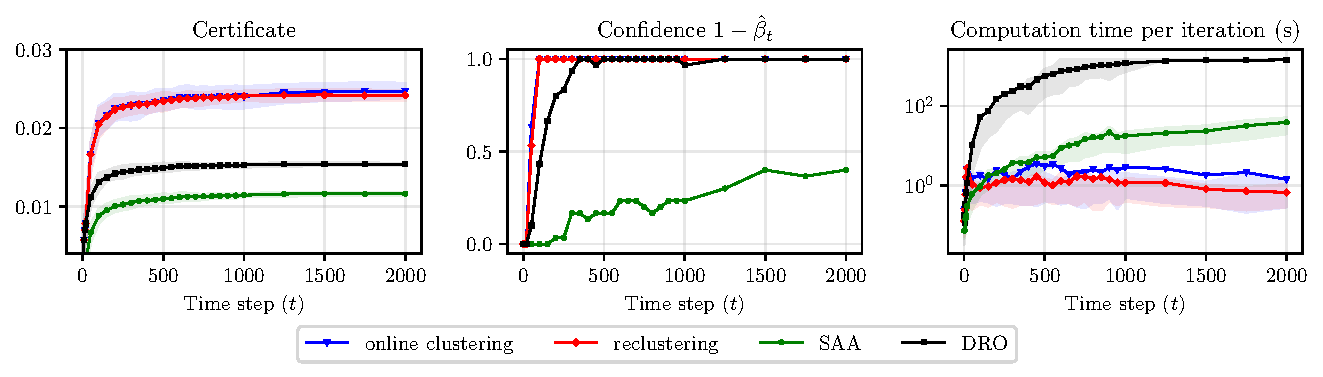
\includegraphics[width = \textwidth]{figures/obj_analysis25.pdf}
	\caption{Sparse portfolio, $K=25$. In-sample certificates, empirical confidence, and per-iteration computation times for the different methods, at $\eps_t = 0.0025{(t+n_0)^{-1/40}}$.}%
	\label{fig:port_obj}%
    \ifpreprint\else
    \vspace{-1em}\fi
\end{figure}
\begin{figure}[ht]%
\vspace{-0.2em}
	\centering
  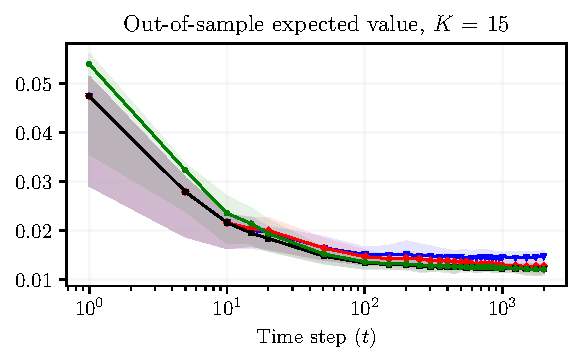
\includegraphics[width = 0.45\textwidth]{figures/eval_analysis_15.pdf}
  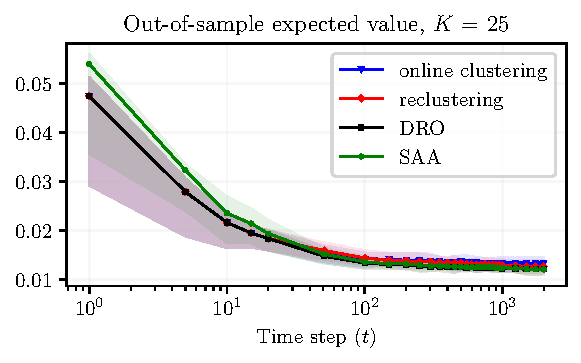
\includegraphics[width = 0.45\textwidth]{figures/eval_analysis_25.pdf}
	\caption{Sparse portfolio. Left: $K = 15$, right: $K = 25$. Out-of-sample expected values for $\epsnom_t = 0.0025{(t+n_0)^{-1/40}}$.}%
	\label{fig:port_eval}%
    \ifpreprint 
    \else
    \vspace{-1em}\fi
\end{figure}
\paragraph{Results}
\RC{For all~\gls{DRO} settings, the radius we obtain through cross-validation is  $\epsnom_t = 0.0025{(t+n_0)^{-1/40}}$.
In Figure~\ref{fig:port_obj}, we compare the certificates, empirical confidence, and per-iteration computation times at the chosen $\epsnom_t$ sequence, and in Figure~\ref{fig:port_eval}, compare the out-of-sample performance. 
We observe that our online data-compressed approaches introduce slight sub-optimality in out-of-sample performance, but provide high-confidence certificates, and offer significant speed-ups compared to nominal~\gls{DRO}. 
As expected, $K=25$ clusters out-performs $K=15$ clusters, but $K=15$ already gives a good approximation of the nominal \gls{DRO} performance.
% For all methods, initializing with a smaller dataset results in worse initial performances, though the robust approaches are able to obtain a good certificate relatively fast. 
The~\gls{SAA} approach improves in performance as the number data points increases, but does not offer a certificate of optimality: the empirical confidence is near 0 for all $t$. Furthermore, it also grows in complexity with sample size and is less efficient than our online approaches. In the long-term, the computation times for our data-compressed approaches can be multiple orders of magnitude faster than that of both~\gls{SAA} and nominal~\gls{DRO}. 
% Surprisingly, as $K=15$ allows for a smaller choice of $\epsnom_t$, the solution times are faster than that of $K=5$. 
We find that the $k$-means warm-starting algorithm (reclustering approach) is particularly efficient, achieving lower computation times and better solution quality than the online clustering method, which entails an extra trade-off between optimality and memory efficiency. Nonetheless, the differences are minimal.}
% We observe that the $k$-means warm-starting algorithm (reclustering approach) is especially efficient, with a lower computation time than even the online clustering approach. The reclustering approach also outperforms the online clustering approach in solution quality, as the latter introduces an additional trade-off between optimality and memory-efficiency. However, the differences in the certificates are minimal. 

\RC{In Figure~\ref{fig:port_regret}, we show the various certificates given in equation~\eqref{eq:is_bounds} (disregarding~$\rho_t$ in favor of cross-validation), and note that the relationships follow the hierarchy presented. The data-compressed in-sample objective value for this maximum-of-affine problem is lower than the in-sample objective of nominal~\gls{DRO}, but adding the clustering discrepancy makes it a valid certificate. We also show the clustering values for a longer horizon, up to $T=10000$, with $\tau = 8500$. 
We observe that the $\barp=1$ and $\barp=2$ clustering distances, $\ld^K_{t,1}$ and $(D^K_{t,2})^2$, as well as $\Phi^K_t$, are converging. 
Moreover, $\ld^K_{t,1} \ge \Phi^K_t$ and, hence, $\max_{j\leq J}M_j\ld^K_{\star,1} \ge \Phi^K_t$  where the maximum Lipschitz constant is $M_1 = 1/\omega = 5$.} This illustrates the relative optimality of $\Phi^K_t$, as opposed to the Wasserstein-1 distance, as proven in Theorem~\ref{cor:opt_cluster}.  
In fact, although we have not assumed (or achieved) optimal clustering-induced coupling, the result still held.
\begin{figure}[ht]%
\vspace{-0.8em}
	\centering
  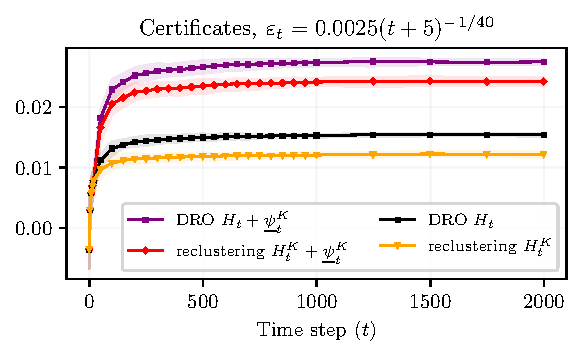
\includegraphics[width = 0.45\textwidth]{figures/bounds_analysis.pdf}
  % 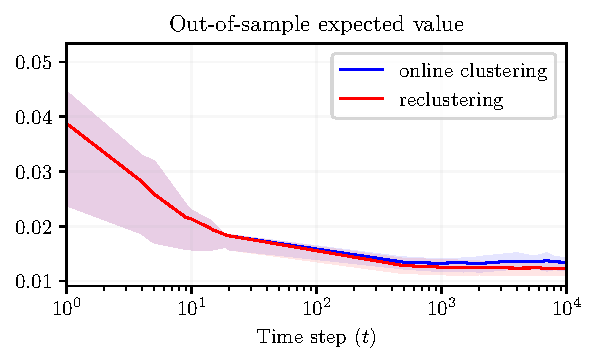
\includegraphics[width = 0.3\textwidth]{figures/eval_analysis_T.pdf}
 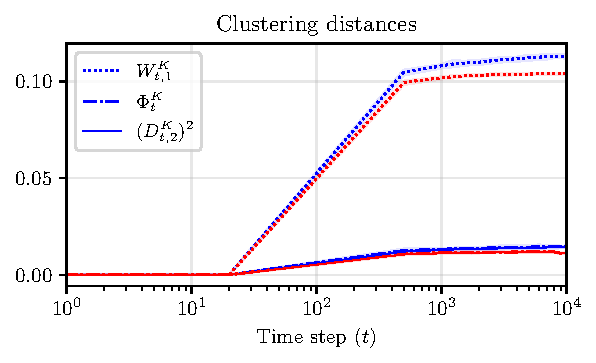
\includegraphics[width = 0.45\textwidth]{figures/dist_conv_W.pdf}
	\caption{Sparse portfolio, $K = 25$. The radius $\epsnom_t = 0.0025{(t+n_0)^{-1/40}}$ for all methods.  Left: certificates from~\eqref{eq:is_bounds}. 
   Right: clustering distances given in Definition~\ref{def:cluster_value}, with $T= 10000$. The lighter (red) shade is for the reclustering method. }%
	\label{fig:port_regret}%
    \ifpreprint 
    \else
    \vspace{-1em}\fi
\end{figure}




% \ifpreprint
% In Figure~\ref{fig:port_regret}, we show the various certificates given in equation~\eqref{eq:is_bounds}, and note that the relationships follow the hierarchy presented. The data-compressed in-sample objective value for this maximum-of-affine problem is lower than the in-sample objective of nominal~\gls{DRO}, but adding the clustering discrepancy makes it a valid certificate.
% % As shown, the upper bounds are generally conservative. Therefore, in practice we tune $\epsnom_t$ using the in-sample value $H^K_t$ instead.  
% \begin{figure}[ht]%
% \vspace{-0.8em}
% 	\centering
%   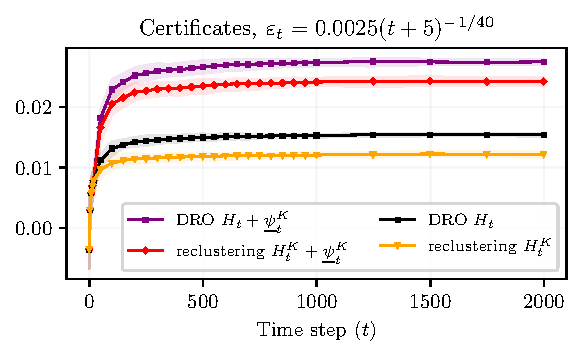
\includegraphics[width = 0.49\textwidth]{figures/bounds_analysis.pdf}
%   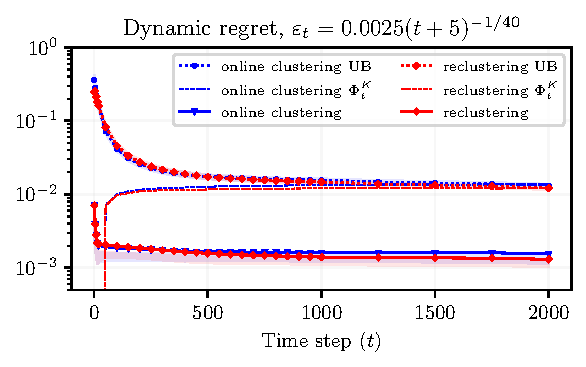
\includegraphics[width = 0.49\textwidth]{figures/regret_analysis.pdf}
% 	\caption{Sparse portfolio, $K = 25$. The radius $\epsnom_t = 0.0025{(t+n_0)^{-1/40}}$ for all methods.  Left: certificates from~\eqref{eq:is_bounds}. 
%     Right: dynamic regret~\eqref{regret}, compared to the theoretical upper bounds.}%
% 	\label{fig:port_regret}%
%     \ifpreprint 
%     \else
%     \vspace{-1em}\fi
% \end{figure}
% In Figure~\ref{fig:port_regret}, we also show the dynamic regret $R(T,K)$ and the regret bound as calculated in Lemma~\ref{lem:regret}. As $T\to\infty$, the upper bound is expected to converge to a fixed function of the clustering discrepancy; indeed, we observe that it coincides with $\Phi^K_t$.
% % converges to $\Phi^K_\star$. 
% This is in line with the theory; since we are solving a maximum-of-affine problem, the term $\bar{\psi}^K_t$ is reduced to 0. 
% \fi
% \ifpreprint 
% The limiting distance becomes $\Phi^K_t$, which, as we show in Figure~\ref{fig:converge} below, is a tighter bound than the Wasserstein-1 distance. This value should converge to its theoretical limit $\Phi_\star^K$.
% \begin{figure}[ht]%
% \vspace{-0.5em}
% 	\centering
%      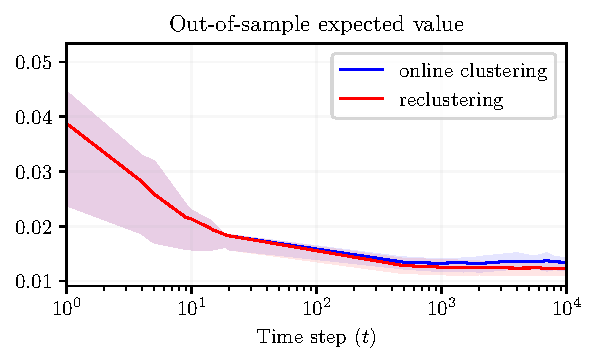
\includegraphics[width = 0.49\textwidth]{figures/eval_analysis_T.pdf}
%  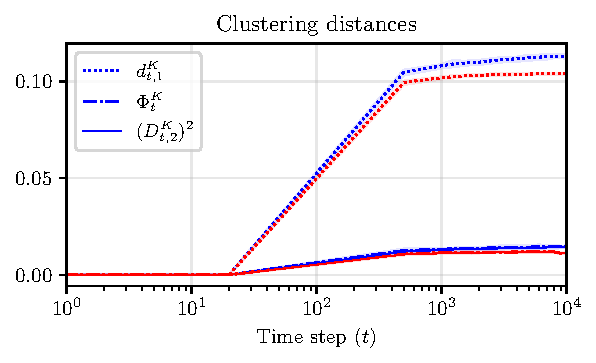
\includegraphics[width = 0.49\textwidth]{figures/dist_conv.pdf}
% 	\caption{Sparse portfolio, $K = 25$, $T=10000$, at $\epsnom_t = 0.0025{(t+n_0)^{-1/40}}$. Left: in-sample certificates. Right: clustering distances given in Definition~\ref{def:cluster_value}.}%
% 	\label{fig:converge}%
%         \ifpreprint \else\vspace{-1em}\fi
% \end{figure}

% In Figure~\ref{fig:converge}, we show the results of our online approaches for a longer horizon, up to $T=10000$, with $\tau = 8500$. 
% We observe that the $\barp=1$ and $\barp=2$ clustering distances, $d^K_{t,1}$ and $(D^K_{t,2})^2$, as well as $\Phi^K_t$, are converging, and the out-of-sample performances are also converging in mean. 
% As remarked above, we observe that $d^K_{t,1}$ upper bounds $\Phi^K_t$ without even multiplying by the maximum Lipschitz constant (which is $1/\alpha = 5$). This illustrates the relative optimality of $\Phi^K_t$, as opposed to the Wasserstein-1 distance, as proven in Theorem~\ref{cor:opt_cluster}.  
% In fact, although we have not assumed (or achieved) optimal clustering-induced coupling, the result still held.
% % \else 
% % The limiting distance becomes $\Phi^K_t$, which, for this example, is a tighter bound than the Wasserstein-1 distance.
% \fi
% % Again, the online clustering approach is slighty suboptimal compared to reclustering, due to the additional trade-off between optimality and memory-efficiency. 
% % However, it still provides a good approximation. 



% \begin{figure}[ht]%
% 	\centering
%  \includegraphics[width = \textwidth]{figures/time_iters.pdf}
% 	\caption{Sparse portfolio, $K = 15$, $n_0=50$. Per-iteration and cumulative computation times for the different methods, at the sequences of $\eps_t$ given in Table~\ref{tab:eps}. The total time for the certificate $\hat{H}^K_t$ is the sum of both reclustering times. \bnote{just plot total time in red}. \bnote{remove cumulative time. remove out of sample plots}}%
% 	\label{fig:port_time}%
% \end{figure}

\ifpreprint
\section{Conclusions}
\label{sec:conclusions}
We have introduced an online data compression framework for solving Wasserstein~\gls{DRO} problems with streaming data. 
Our method constructs adaptive ambiguity sets using online clustering, allowing the uncertainty model to evolve as new data arrives, while maintaining out-of-sample performance guarantees. 
We analyzed the impact of data compression on solution quality, providing finite-sample and asymptotic performance bounds that relate to nominal bounds for Wasserstein~\gls{DRO}.
% as well as a sublinear regret analysis with respect to the full-information \gls{DRO} solution. 
The framework is compatible with a broad class of clustering algorithms and supports efficient, memory-aware implementations. 
Numerical experiments in sparse portfolio optimization demonstrate significant computational savings with minimal loss in solution quality.

\section*{Acknowledgments}
\myack
\fi


\ifpreprint
\bibliography{references}
\fi 
% \else
% % Acknowledgments here
% \begin{acknowledgements}
% \fi
% The simulations presented in this article were performed on computational resources managed and supported by Princeton Research Computing, a consortium of groups including the Princeton Institute for Computational Science and Engineering (PICSciE) and the Office of Information Technology's High Performance Computing Center and Visualization Laboratory at Princeton University.
% \ifpreprint \else
% \end{acknowledgements}
% \fi

% \ifpreprint \else
% \section*{Statements and Declarations}
% \paragraph{Competing Interests.}
% The authors have no relevant financial or non-financial interests to disclose.
%
% \fi



\appendix
\ifpreprint
\section{Appendices}
\fi

\ifpreprint
\subsection{Proof of the performance guarantees in Section~\ref{sec:gen_gau}}
\else
\section{Proof of the performance guarantees in Section~\ref{sec:gen_gau}}
\fi
\label{app:gen_proofs}
\begin{proof}[Proof of Lemma~\ref{lem:delta}]
    For all $t$, let $\tilde{\mathbf{Q}}_t \in  \tilde{\mathbf{B}}_{\epsnom_t}^{r}(\hat{\prob}_t)$ and $\mathbf{Q}_t \in  \mathcal{P}_t$. By~\cite[Lemma 3.7]{mohajerin2018data}, we observe {$\prob^{\infty}\{ \lim_{t\to\infty}\tilde{\mathbf{Q}}_t \rightarrow  \prob\}=1$} and $\prob^{\infty}\left\{ \lim_{t\to\infty}\mathbf{Q}_t \rightarrow \prob \right \}=1$. \RC{The first result follows. 
    If $f$ is Lipschitz, by the Kantorovich-Rubinstein duality~\cite{kantorovich_duality}, and by noting $W_1(\tilde{\mathbf{Q}}_t,\mathbf{Q}_t)\leq W_r(\tilde{\mathbf{Q}}_t,\mathbf{Q}_t) \leq 2\epsnom_{t}$ (by the ordering of Wasserstein distances and the triangle inequality), we obtain $\Delta_t\leq 2\max_{j\leq J}M_j \epsnom_{t}$.}
    \RC{If $f$ is $L$-smooth, then by the descent lemma and~\eqref{def:wass}, 
    $\mathbf{E}_{\mathbf{\tilde{Q}_t}}[f(\unc, x_{t})] - \mathbf{E}_{\mathbf{{Q}_t}}[f(\unc, x_{t})] \leq \inf_{\pi \in \Pi(\tilde{\mathbf{Q}}_t,\mathbf{Q}_t)}\int_{S\times S} \nabla f(v,x_t)^T(u-v)d\pi(u,v) + (L/2)W_2(\tilde{\mathbf{Q}}_t,\mathbf{Q}_t)^2.$ By the Cauchy-Schwartz inequality and H\"{o}lder's inequality with order 2, the integral is upper bounded by $(\textstyle \int \|\nabla f(v,x_t)\|^2d{\mathbf{Q}}_t)^{1/2} (\int \|u-v\|^2d\pi(u,v))^{1/2} = \|\nabla f_{x_t}\|_{L_2({\mathbf{Q}}_t)}W_2(\tilde{\mathbf{Q}}_t,\mathbf{Q}_t)$. When $r\geq 2$, this simplifies to $\Delta_t \leq \|\nabla f_{x_t}\|_{L_2({\mathbf{Q}}_t)}2\epsnom_t + 2L\epsnom_t^2$. The result follows.}
\end{proof}

\begin{proof}[Proof of Theorem~\ref{thm:nominal_performance}]
\RC{We first prove~\eqref{eq:relate}. We begin by observing} 
\begin{equation*}
    H_t = \max_{\mathbf{Q} \in \mathcal{P}_{t}} \mathbf{E}_{\mathbf{Q}}[f( \unc,x_t)] \leq \max_{\mathbf{Q} \in \mathcal{P}_{t}} \mathbf{E}_{\mathbf{Q}}[f(\unc, x^K_{t})] \leq \max_{\mathbf{Q} \in \mathcal{P}^K_{t}} \mathbf{E}_{\mathbf{Q}}[f(\unc, x^K_{t})]  + \Phi^K_{t},
\end{equation*}
with $\max_{\mathbf{Q} \in \mathcal{P}^K_{t}}\mathbf{E}_{\mathbf{Q}}[f(\unc, x^K_{t})] = H^K_t$ in the final clause. 
The first inequality follows from the optimality of $x_t$, the second follows from~\cite[Theorem 5]{mro}, 
% the equality follows from the optimality of $x^K_{t}$, 
and $\Phi^K_t$ is defined in Definition~\ref{def:cluster_value}.
From~\cite[Theorem 4]{mro}, we note that $\Phi^K_{t}=0$ for concave functions $f$,~\ie, when $J=1$.
\RC{When $f$ is Lipschitz, using Kantorovich-Rubinstein duality~\cite{kantorovich_duality}, we can obtain a second bound on $H_t$,}
\begin{equation*}
\begin{aligned}
        \max_{\mathbf{Q} \in \mathcal{P}_{t}} \mathbf{E}_{\mathbf{Q}}[f(\unc, x^K_{t})] &\leq  \max_{\mathbf{Q} \in \mathcal{P}^K_{t}} \mathbf{E}_{\mathbf{Q}}[f(\unc, x^K_{t})] + \max_{j\leq J}M_j(2\epsnom_{t} + W_1(\hat{\prob}_{t},\hat{\prob}^K_{t})).
    % &\leq H^K_t+ \max_{j\leq J}M_j(2\epsnom_{t} +d^K_{t,1}).\\ 
    \end{aligned}
\end{equation*}
\RC{When $f$ is $L$-smooth, using the same procedure as in the proof of Lemma~\ref{lem:delta} above, we obtain a third bound in terms of the $W_2$ distance.} 
\RC{Combining all gives the bound on $H_t - H^K_t$.} For the other side, from the optimality of $H^K_t$ and \cite[Theorem 5]{mro},
\begin{equation*}
\begin{aligned}
    H^K_t \leq \max_{\mathbf{Q} \in \mathcal{P}^K_{t}} \mathbf{E}_{\mathbf{Q}}[f(\unc, x_{t})] &\leq  H_t + (\tilde{H}_t - H_t) + {\max_{j \leq J}\frac{L_j}{2}}(D^K_{t,2})^2,
    % &= H_t + \Delta_t + {\max_{j \leq J}(L_j/2)}(D^K_{t,2})^2,
\end{aligned}
\end{equation*}
where $\tilde{H}_t - H_t =\Delta_t$ is given in Lemma~\ref{lem:delta}. 
Kantorovich-Rubinstein duality yields 
\begin{equation*} H^K_t \leq \max_{\mathbf{Q} \in \mathcal{P}^K_{t}} \mathbf{E}_{\mathbf{Q}}[f(\unc, x_{t})] \leq H_t + \max_{j\leq J}M_j(2\epsnom_{t} +\ld^K_{t,1}).\end{equation*}
\RC{Combining everything, we obtain~\eqref{eq:relate}.} \RC{Using these relationships, and the finite-sample performance guarantee~\eqref{eq:prob_guarantees1} implied by the chosen radii sequence in Assumption~\ref{ass:general_ass}(1), we obtain~\eqref{eq:is_bounds}.} \RC{To prove~\eqref{eq:oos_bounds}, we note that if the radii are chosen using Theorem~\ref{thm:calc_eps}, then with probability $1 - \beta_{t}$, $\prob \in \mathcal{P}_{t},$ and we have, with $\rho_{t}=0$,}
\begin{equation}
\label{eq:oos_proof}
        \prob^{{t}}\left( H_\star \leq \mathbf{E}_{\mathbf{P}}[f(\unc, x^K_{t})] \leq \max_{\mathbf{Q} \in \mathcal{P}_{t}} \mathbf{E}_{\mathbf{Q}}[f(\unc, x^K_{t})] + \rho_{t}\right) \geq 1 - \beta_{t}.
\end{equation}
\RC{Applying the bounds we derived for $\max_{\mathbf{Q} \in \mathcal{P}_{t}} \mathbf{E}_{\mathbf{Q}}[f(\unc, x^K_{t})]$ gives the desired result.} \RC{If the radii are chosen using Theorem~\ref{thm:informal_curse}, then as $x^K_t \in \mathcal{X}$,~\eqref{eq:oos_proof} holds by~\eqref{eq:informal_x}.}
\end{proof}
\ifsiam
\newpage
\fi
% \IrinaNote{Rewrite}
% Recall that under the radius $\epsnom_{t-1}$, the solution $x_t$  and optimal value $H_t = \max_{\mathbf{Q} \in \mathcal{P}_{t-1}} \mathbf{E}_{\mathbf{Q}}[f( \unc,x_t)]$ of the \gls{DRO} problem~\eqref{eq:DRO} imply the finite sample performance guarantee~\eqref{eq:prob_guarantees1}.
% % $$\prob^{n_{t-1}}\left(H_\star \leq \max_{\mathbf{Q} \in \mathcal{P}_{t-1}} \mathbf{E}_{\mathbf{Q}}[f(\unc,x_t)] = H_t \right) \geq 1 - \beta_{t-1}.$$
% % Furthermore, when the adaptive ambiguity set has radius $\eps_{t-1} = \epsnom_{t-1}$, the solution $x^K_{t}$ and optimal value $H^K_t$ of the compressed \gls{DRO} problem~\eqref{eq:dro:time} satisfy
% We also observe
% \begin{equation*}
%     \begin{aligned}
%     \max_{\mathbf{Q} \in \mathcal{P}_{t-1}} \mathbf{E}_{\mathbf{Q}}[f( \unc,x_t)] \leq \max_{\mathbf{Q} \in \mathcal{P}_{t-1}} \mathbf{E}_{\mathbf{Q}}[f(\unc, x^K_{t})] &\leq \max_{\mathbf{Q} \in \mathcal{P}^K_{t-1}} \mathbf{E}_{\mathbf{Q}}[f(\unc, x^K_{t})]  + \Phi^K_{t-1},
%     \end{aligned}
% \end{equation*}
% with $\max_{\mathbf{Q} \in \mathcal{P}^K_{t-1}}\mathbf{E}_{\mathbf{Q}}[f(\unc, x^K_{t})] = H^K_t$ in the final clause. 
% The first inequality follows from the optimality of $x_t$, the second follows from~\cite[Theorem 5]{mro}, 
% % the equality follows from the optimality of $x^K_{t}$, 
% and $\Phi^K_t$ is defined in Definition~\ref{def:cluster_value}.
% From~\cite[Theorem 4]{mro}, we note that $\Phi^K_{t-1}=0$ for concave functions $f$,~\ie, when $J=1$.
% We also observe, using Kantorovich-Rubinstein duality~\cite{kantorovich_duality}, 
% \begin{equation*}
% \begin{aligned}
%         \max_{\mathbf{Q} \in \mathcal{P}_{t-1}} \mathbf{E}_{\mathbf{Q}}[f(\unc, x^K_{t})] &\leq  \max_{\mathbf{Q} \in \mathcal{P}^K_{t-1}} \mathbf{E}_{\mathbf{Q}}[f(\unc, x^K_{t})] + \max_{j\leq J}M_j(2\epsnom_{t-1} + W_1(\hat{\prob}_{t-1},\hat{\prob}^K_{t-1})) \\
%     &\leq H^K_t+ \max_{j\leq J}M_j(2\epsnom_{t-1} +d^K_{t-1,1}).\\ 
%     \end{aligned}
% \end{equation*}
% Combining the above relations, we obtain the first half of equation~\eqref{eq:is_bounds}, 
% $$\prob^{{t-1}}\left(H_\star \leq H_t \leq H^K_t + \min\left\{\Phi^K_{t-1},\max_{j\leq J}M_j(2\epsnom_{t-1} +d^K_{t-1,1})\right\}\right) \geq 1 - \beta_{t-1}.$$
% % Note that by definition of $\Phi^K_{t-1}$, it is generally expected to be a lower bound of $\max_{j\leq J}M_j(2\epsnom_{t-1} + d^K_{t-1,1}$), as each $M_j$ is assumed to be the global Lipchitz constant that bounds the functional change $|f_j(x,u) - f_j(x,v)|$, $u,v\in \supp$. However, since $d^K_{t-1,1}$ assumes optimal coupling between the two empirical distributions, and $\Phi^K_t$ uses the coupling induced by clustering, there may be exceptions. 

% To derive~\eqref{eq:oos_bounds}, we also note that, with probability $1 - \beta_{t-1}$,
% \begin{equation*}
%     \begin{aligned}
%         H_\star = \min_{x\in \mathcal{X}} \mathbf{E}_{\mathbf{P}}[f(\unc,x)] \leq \mathbf{E}_{\mathbf{P}}[f(\unc, x^K_{t})] \leq \max_{\mathbf{Q} \in \mathcal{P}_{t-1}} \mathbf{E}_{\mathbf{Q}}[f(\unc, x^K_{t})].
%     \end{aligned}
% \end{equation*}
% Now for the upper bound, from the optimality of $H^K_t$ and \cite[Theorem 5]{mro},
% \begin{equation*}
% \begin{aligned}
%     H^K_t \leq \max_{\mathbf{Q} \in \mathcal{P}^K_{t-1}} \mathbf{E}_{\mathbf{Q}}[f(\unc, x_{t})] &\leq  H_t + (\tilde{H}_t - H_t) + {\max_{j \leq J}(L_j/2)}(D^K_{t-1,2})^2\\
%     &= H_t + \Delta_t + {\max_{j \leq J}(L_j/2)}(D^K_{t-1,2})^2,
% \end{aligned}
% \end{equation*}
% where $\Delta_t$ is given in Lemma~\ref{lem:delta}. 
% By applying Kantorovich-Rubinstein duality, 
% $$ H^K_t \leq \max_{\mathbf{Q} \in \mathcal{P}^K_{t-1}} \mathbf{E}_{\mathbf{Q}}[f(\unc, x_{t})] \leq H_t + \max_{j\leq J}M_j(2\epsnom_{t-1} +d^K_{t-1,1}).$$
% Combining both inequalities, we obtain 
% $$H^K_t \leq H_t + \min\left\{\Delta_t + {\max_{j \leq J}(L_j/2)}(D^K_{t-1,2})^2,\max_{j\leq J}M_j(2\epsnom_{t-1} +d^K_{t-1,1})\right\}.$$
% \ifpreprint Combining the upper and lower bounds gives the desired result.\fi
% Rearranging terms and combining with previous results give equations~\eqref{eq:relate} and~\eqref{eq:is_bounds}.
% \end{proof}

% \ifpreprint
% \ifpreprint
% \subsection{Proof of the regret bound in Section~\ref{sec:regret}}
% \else
% \section{Proof of the regret bounds in Section~\ref{sec:regret}}
% \fi
% \label{app:regret}
% \begin{proof}[Proof of Lemma~\ref{lem:regret}]
% For brevity, let us denote the following shorthands:
%  $\bar{f}_t(x) = \max_{\mathbf{Q} \in \mathcal{P}_t} \mathbf{E}_{\mathbf{Q}}[f(\unc,x)]$, $\bar{f}^K_t(x) = \max_{\mathbf{Q} \in \mathcal{P}^K_{t-1}} \mathbf{E}_{\mathbf{Q}}[f(\unc,x)],$ 
%  and the corresponding solutions 
%  $x_t = \argmin_{x \in \mathcal{X}}\bar{f}_t(x)$, $x^K_{t} = \argmin_{x \in \mathcal{X}}\bar{f}^K_{t}(x).$
% We wish to bound 
% $R(T) = (1/T)\sum_{t=1}^T \left(\bar{f}_t(x^K_{t}) - \bar{f}_t(x_t)\right),$
% which can be rewritten as
% \begin{equation*}
% \begin{aligned}
%   R(T,K) &=\frac{1}{T}\sum_{t=1}^T \left(\bar{f}_t(x^K_{t}) - \bar{f}_{t-1}(x_{t-1})\right) + \frac{1}{T}\sum_{t=1}^T \left( \bar{f}_{t-1}(x_{t}) - \bar{f}_t(x_t)\right).
% \end{aligned}
% \end{equation*}
% Note that the second summation telescopes to $(1/T)\left( \bar{f}_{0}(x_{0}) - \bar{f}_T(x_T)\right).$
% We then begin by bounding the terms in the first summation. We observe that
% $$\bar{f}_t(x^K_{t}) \leq \bar{f}^K_{t+1}(x^K_{t}) + \min\left\{ \Phi^K_t,  \max_{j\leq J}M_j(2\epsnom_t+d^K_{t,1})\right\} = \bar{f}^K_{t+1}(x^K_{t}) + \underline{\psi}_{t+1}^K,$$
% using~\cite[Theorem 5]{mro} and Kantorovich-Rubinstein duality. Using the same theorems, we observe
% $\bar{f}_{t-1}(x_{t-1}) \geq \bar{f}_{t}^K(x_{t-1}) - \bar{\psi}_t^K,$
% and by the optimality of $x^K_{t}$ for the particular problem, $\bar{f}_{t}^K(x_{t-1}) \geq \bar{f}_{t}^K(x^K_{t})$.
% Furthermore, by Kantorovich-Rubinstein duality
% $$ \bar{f}^K_{t+1}(x^K_{t}) -\bar{f}_{t}^K(x^K_{t}) \leq \max_{j\leq J}M_j(2\epsnom_{t-1} + W_1(\hat{\prob}^K_t,\hat{\prob}^K_{t-1})).$$
% Combining these relations, we obtain
%     \begin{equation}
%     \begin{aligned}
%     \label{lem:regret_eq}
%     \frac{1}{T}& \sum_{t=1}^T (\bar{f}_t(x^K_{t}) - \bar{f}_{t-1}(x_{t-1})) \leq \frac{1}{T}\sum_{t=1}^T  (\underline{\psi}_{t+1}^K + \bar{\psi}_t^K  + \max_{j\leq J}M_j(2\epsnom_{t-1} +W_1(\hat{\prob}^K_t,\hat{\prob}^K_{t-1})).
%     \end{aligned}
%     \end{equation} 
% For the final term, we show again by Kantorovich-Rubinstein duality
% $$\bar{f}_{0}(x_{0}) - \bar{f}_T(x_T) \leq \bar{f}_{0}(x_{T}) - \bar{f}_T(x_T)\leq  \max_{j\leq J}M_j(\epsnom_0 + \epsnom_T +W_1(\hat{\prob}^0,\hat{\prob}_t)).$$
% \end{proof}

% \ifpreprint
% We use this to prove Theorem~\ref{thm:regret} and its corollaries. 
% \fi
% \begin{proof}[Proof of Theorem~\ref{thm:regret} and Corollary~\ref{cor:regret_beta}]
% We examine the terms in $R(T,K)$ individually, for a finite value $T \gg \tau$.
% As we assume the Lipschitz condition, we use the corresponding terms in $\underline{\psi}^K_{t-1}$ and $\bar{\psi}^K_t$ as the upper bounds. 
% % We first examine the terms on the right-hand-side of the minimum clauses. 
% By assumption, $\epsnom_t\sim (\log(\beta_t^{-1})/t)^{1/d}$, so their averages are $O((\log(\beta_T^{-1})/T)^{1/d}).$
% Note that by the summability of $\beta_t$, the convergence rate of $\beta_t$ is at least sublinear. 
% Next, recall by the triangle inequality,  $$d^K_{t,1} \leq W_1(\hat{\prob}_t,\prob) + W_1(\prob,\prob^K_\star) + W_1(\prob^K_\star,\prob^K_{t}).$$ By Theorem~\ref{thm:calc_eps}, we can construct a summable sequence $\beta_t$ such that $\prob(W_1(\hat{\prob}_t,\prob) \leq \epsnom_t) \geq  1-\beta_t$, where $\epsnom_t$ is the same as above. By Theorem~\ref{lem:conditional_Conv}, a similar result holds for $W_1(\prob^K_\star,\hat{\prob}^K_t)$, with a sequence of radii $\tilde{\epsnom}_t\leq O(\epsnom_t)$ for $t \geq \tau$. Since $T \gg \tau$, the finite values $\tilde{\epsnom}_t/T$ for $t\leq \tau$ are dominated by $O(\epsnom_T)$.
% Therefore, the terms involving $d^K_{t,1}$ and $d^K_{t-1,1}$ are together $O(W_1(\prob,\prob^K_\star) + \left(\log(\beta_{T}^{-1})/T\right)^{1/d})$, with probability at least $\Pi_{t=0}^{T-1}(1-\beta_t)^2$. This probability can be constructed to converge to a nonzero value due to the summability of $\beta_t$. 
% % Now, we note the terms on the left-hand-side of the minimum clauses. These terms quantify the distances between the empirical and the compressed empirical distributions, $\hat{\prob}_t$ and $\hat{\prob}^K_t$, at times $t$ and $t-1$. They converge to their asymptotic values at the convergence rates of $W_1(\hat{\prob}_t,\prob)$ and $W_1(\prob^K_\star,\prob^K_{t})$, which, as shown above, is $O(\epsnom_t)$. 
% % Overall, then, the sum of the two minimum clauses are bounded by $O\left(\underline{\psi}_\star^K + \bar{\psi}_\star^K\right)$ + $O(\epsnom_t)$.
% Next, we note again by the triangle inequality, $$W_1(\hat{\prob}^0,\hat{\prob}_t) \leq W_1(\hat{\prob}^0,\prob) + W_1(\prob,\hat{\prob}_t),$$
% where the first term is constant in $T$ and the second term, by measure concentration results, is upper bounded by $\epsnom_T$ with some probability $1-\beta_T$. Therefore, with probability $1-\beta_T$, $W_1(\hat{\prob}^0,\hat{\prob}_t)/T$ is $O(T^{-1})$.
% Lastly, by the triangle inequality,
% $$W_1(\hat{\prob}^K_t,\hat{\prob}^K_{t-1}) \leq W_1(\hat{\prob}^K_t,\prob^K_\star) + W_1(\prob^K_\star,\hat{\prob}^K_{t-1}) \leq 2\tilde{\epsnom}_{t-1},$$
% with probability $(1-\beta_{t-1})^2$.
% The average over $T$ is again $O(\epsnom_{T})$, with probability $\Pi_{t=0}^{T-1}(1-\beta_t)^2$.
% Combining all terms, we have $R(T,K) \leq O(\left(\log(\beta_T^{-1})/T\right)^{1/d})+ O(W_1(\prob,\prob^K_\star))$, with a consolidated probability $1-\zeta \geq \Pi_{t=0}^T(1-\beta_t)^4$. Again, we remark that the probability $1-\zeta$ can be constructed to be high, with well-chosen sequences $\beta_t$ and $\epsnom_t$. Note that their convergence rates are inversely related; the higher the desired probability $1-\zeta$, the slower the convergence with respect to $T$. Using the Bonferroni Inequality~\cite{Bonferroni}, the probability can be estimated as $1-\zeta \geq 1-\sum_{t=0}^T4\beta_t$.

% Corollary~\ref{cor:regret_beta} follows by setting $\beta_t = O(\exp(-\sqrt{n_t})$ and simplifying.
% \end{proof}


% \begin{proof}[Proof of Corollary~\ref{cor:regret}]
% \ifpreprint
%     The asymptotic result for $T \rightarrow \infty$ follows from Lemma~\ref{lem:regret} and the results from Section~\ref{sec:general}.
%     \fi As $t \to \infty$ and $T\to\infty$, by the almost sure convergence of 
%      $\underline{\psi}_t^K + \bar{\psi}_t^K$ to $\underline{\psi}_\star^K + \bar{\psi}_\star^K$,
%     % $d^K_{t,1}$ to $W_1(\prob,\prob^K_\star)$, 
%     $W_1(\hat{\prob}^0,\hat{\prob}_t)/T$ to $W_1(\hat{\prob}^0,{\prob})/T$ to $0$, and $ W_1(\hat{\prob}^K_t,\hat{\prob}^K_{t-1})$ to $0$, by the Ces\`aro Mean Theorem~\cite{cesaro}, 
%     $R(T,K)$ converges to some value that is $O(\underline{\psi}_
%     \star^K + \bar{\psi}_\star^K)$ with probability 1. 
% The result for $K \rightarrow \infty$ follows from Theorem~\ref{thm:clustering_conv}.
% \end{proof}
% \fi

% \ifpreprint
\ifpreprint
\subsection{Proofs of Section~\ref{sec:bounded_perf} results}
\else
\section{Proofs of Section~\ref{sec:bounded_perf} results}
\fi
\label{app:bounded_perf_1}
\begin{proof}[Proof of Lemma~\ref{lem:dist}]
% Let the center of the $k$-th cluster be $a^k$.
By definition of the Wasserstein metric,
\begin{equation*}
\begin{aligned}
(\ld^K_{t,p})^p = W_p(\hat{\prob}_t, \hat{\mathbf{P}}^K_t)^p & = \inf_{\pi \in \Pi}\left \{\int_{{\supp}^2} \|\unc - \unc^\prime\|^p\pi(d\unc, d\unc^\prime)\right\}\\
& \leq \sum_{k=1}^K \frac{n^t_k}{n_t} \int_{\supp^2}\|\unc-\bar{u}^k_t\|^p \hat{\prob}_t(\unc|\unc^\prime = \bar{u}^k_t)(du)\\
& \leq \sum_{k=1}^K \frac{n_k^t}{n_t} \frac{1}{n_k^t} \sum_{ \hat{\unc}\in C^k_t}\|\hat{\unc} - \bar{u}^k_t\|^p\\
& = \frac{1}{n_t}  \sum_{k=1}^K\sum_{\hat{\unc}\in C^k_t}\|\hat{\unc}- \bar{u}^k_t\|^p\\
% & \leq \frac{1}{n_t}  \sum_{k=1}^K\sum_{\hat{\unc}\in C^k_t}(\|\hat{\unc} - a^k\| + \|a^k - \bar{u}^k_t\| )^p\\
& \leq (2\eta_K)^p,
\end{aligned}
\end{equation*}
where the final inequality follows from the cluster diameter of $2\eta_K$, using Definition~\ref{def:diam_cluster}. Next, by exploiting the triangular inequality, with probability $1-\beta$, we get
\begin{equation}\label{eq:MRO}
W_p(\mathbf{P}, \hat{\mathbf{P}}^K_t) \leq W_p(\mathbf{P}, \hat{\prob}_t) + W_p(\hat{\mathbf{P}}_t, \hat{\mathbf{P}}^K_t) \leq \epsnom_t + 2\eta_K,
\end{equation}
where $\epsnom_t$ is computed as in Theorem~\ref{explicit}. 
\end{proof}

\begin{proof}[Proof of Lemma~\ref{lemma:convergence:K}]
As $\mathbf{Q}_t \in \mathbf{B}_{\eps_{t}}(\hat{\mathbf{P}}_{t}^K)$, from the triangular inequality,
$$
W_p(\mathbf{P}, \mathbf{Q}_t) \leq W_p(\mathbf{P}, \hat{\mathbf{P}}^K_{t}) + W_p(\hat{\mathbf{P}}^K_{t}, \mathbf{Q}_t) \leq W_p(\mathbf{P}, \hat{\mathbf{P}}^K_{t}) + \eps_{t} $$
From \eqref{eq:MRO} we have $W_p(\mathbf{P}, \hat{\mathbf{P}}^K_{t}) \leq \epsnom_{t} + 2\eta_K = \eps_{t}$. Thus, we have $\mathbf{P}(W_p(\mathbf{P}, \mathbf{Q}_t) \leq 2\eps_{t}) \geq 1 - \beta_{t}$.
Since by definition $\sum_{t=0}^\infty \beta_t < \infty$, then by the Borel-Cantelli Lemma we get
$$
\mathbf{P}^\infty\{W_p(\mathbf{P}, \mathbf{Q}_t) \leq 2\eps_{t} \text{~~for all large enough $t$}\} = 1.
$$
Since by definition
$\lim_{t \rightarrow \infty} 2\eps_{t} = 4\eta_K$, we conclude $\lim_{t\rightarrow \infty}  W_p(\mathbf{P}, \mathbf{Q}_t) \leq 4\eta_K$ almost surely.
\end{proof}

\ifpreprint
\begin{proof}[Proof of Theorem~\ref{thm:asy_eta}]
By the finite sample performance guarantee in Theorem~\ref{lemma:guarantees_fin} and the summability of $\beta_t$, the Borel–Cantelli Lemma implies that $$ \mathbf{P}^\infty\left\{ H_\star \leq \limsup_{t \rightarrow \infty } \Expect_\prob[f(\unc,x^K_{t})]\leq  \limsup_{t \rightarrow \infty } H^K_t\right\} = 1.$$
Now, choose any $\gamma >0$, and fix a $\gamma$-optimal solution $x_{\gamma} \in \mathcal{X}$ of~\eqref{eq:opt} such that $\Expect_{\prob}[f(x_{\gamma},u)] \leq H_\star + \gamma$. For each $t$, we choose a $\gamma$-optimal distribution $\mathbf{Q}_t \in \mathcal{P}^{t-1}$ such that $ \sup_{\mathbf{Q} \in \mathcal{P}^{t-1}}\Expect_{\mathbf{Q}}[f(x_{\gamma},u)] \leq \Expect_{\mathbf{Q}_t}[f(x_{\gamma},u)] + \gamma.$
Then, we observe that
\begin{equation*}
\begin{aligned}
    \limsup_{t \rightarrow \infty } H^K_t &\leq \limsup_{t \rightarrow \infty } \sup_{\mathbf{Q} \in \mathcal{P}^{t-1}}\Expect_{\mathbf{Q}}[f(x_{\gamma},u)]\\
    &\leq \limsup_{t \rightarrow \infty }\Expect_{\mathbf{Q}_t}[f(x_{\gamma},u)] + \gamma\\
     &\leq \limsup_{t \rightarrow \infty }\Expect_{\mathbf{\prob}}[f(x_{\gamma},u)] + \max_{j\leq J}M_jW_1(\mathbf{Q}_t,\prob)+ \gamma\\
     &\leq H_\star + 4\max_{j\leq J}M_j\eta_K + 2\gamma,
\end{aligned}
\end{equation*}
where the first inequality follows from the optimality of $x^K_{t}$ and $H^K_t$, and the third inequality follows from Kantorovich-Rubinstein duality~\cite{kantorovich_duality} and the Lipschitz condition of $f$. The final inequality follows from Lemma~\ref{lemma:convergence:K}. Since we chose $\gamma > 0$ arbitrarily, we can conclude that
$\limsup_{t \rightarrow \infty } H^K_t \leq H_\star + 4\max_{j\leq J}M_j\eta_K $.
\end{proof}
\fi


\ifpreprint
\subsection{Online clustering algorithm (Section~\ref{sec:clustream})}
\label{app:onlinecluster}
We give details for the online clustering algorithm, introduced in Section~\ref{sec:clustream}.
We keep track of two sets of clusters: a set of $Q \geq K$ {\it microclusters}, and a set of $K$ {\it macroclusters}. 
For simplicity, below we assume the number of microclusters to be $Q$ and the number of macroclusters to be $K$; if the number of datapoints is smaller, \ie, $Q_t \leq Q$ and $K_t \leq K$, the arrival of new datapoints result in new clusters.

% If this is less than $Q$, the microcluster merging step will not occur until the number reaches $Q$.


\paragraph{Initialization}
We initialize the problem by solving approximately the $k$-centers problem~\eqref{def:k_centers} with respect to $\hat{\prob}^0$, allowing up to $Q$ clusters. This set of centers is denoted $A^Q_0$. We assign all points to the closest center, and define the support of the $q$-th cluster $S^q_0$ as the Voronoi region around its center $a_0^q \in A^Q_0$. Note that the Voronoi regions need not be explicitly stored; they are implicitly defined by their centers. 
For each cluster, we note its center, \RC{mean}, root-mean-squared-error (RMSE), and weight. These are denoted the {\it microclusters}. We refer to the RMSE of each cluster as $\eta^q_t$, and for clusters with only a single datapoint, heuristically initialize it as twice the minimum RMSE of all clusters. 
% We also keep a threshold value $\eta$, which could be a given arbitrary value, or a function of the current clustering. For example, we can initialize it as the maximum distance between any data point and its cluster center, $\eta = \max_{\hat{u} \in \mathcal{D}_t}\min_{a\in A^Q_0}{\|\hat{u} - a\|}$, where . 

To create $K$ {\it macroclusters}, we solve approximately the $k$-centers problem with respect to $A^Q_0$, and obtain a set of centers $A^K_0$. Each microcluster is assigned to the macrocluster with the closest center; each macrocluster then contains all the points of its constituent microclusters, and has their combined weight. The \RC{mean} of the macrocluster is therefore the weighted average of the \RC{means} of the constituent microclusters. The support of the $k$-th macrocluster is the Voronoi region around the $k$-th center $a_0^k \in A^K_0$, plus the datapoints assigned to it, and minus the datapoints assigned to other clusters, \ie,
\begin{equation}
\label{eq:update_sup}
    S^k_t = (V(a_t^k) \cup \{C^k_t\})/\{C^{k'}_t\}_{k' \neq k}.
\end{equation}
In this manner, the set of supports $\mathcal{S}_t$ satisfy Assumption~\ref{ass:support}. The necessity of this adjustment of the support follows from the two-layer nature of the clustering algorithm. It is possible for a datapoint to be clustered into the $q$-th microcluster, which is assigned to the $k$-th macrocluster, but distance-wise is actually closer to the center of $k'$-th macrocluster for some $k' \neq k$.

% \bnote{are the next two phrases necessary? }
% We note that we can also initialize the problem with {\it any} $Q$-clustering of the initial dataset~$\mathcal{D}_0$. 
% In the case the clusters overlap, the support of the $q$-th cluster is defined as in~\eqref{eq:update_sup}. 
% However, we require that identical datapoints must be clustered together. 

\paragraph{Online updating procedure}
For $t \geq 1$, when we observe a new datapoint $\hat{u}$, we calculate its distance to the microcluster whose support it falls on, \ie, if it falls on support $S^q_{t-1},$
$$d_t = \|\hat{u} - a^q_{t-1}\|.$$
If this value is below $2\eta^q_{t-1}$, where $\eta^q_{t-1}$ is the RMSE, we assign it to this cluster. The multiplier of 2 is selected according to {\it CluStream} sensitivity analysis~\cite[Section 6.4]{clustream}. We then update all microclusters weights, as well as the \RC{mean} and RMSE of the assigned microcluster. The macroclusters are also adjusted accordingly, based on their constituent microclusters. 

On the other hand, if $d_t > 2\eta^q_{t-1}$, we create a new microcluster with this datapoint as its center, and assign it the weight $1/n_t$. The weights of the other microclusters are decreased accordingly, following~\eqref{eq:cluster_update_dym}. The RMSE of this cluster is initialized heuristically to be twice the minimum RMSE of all other existing clusters. If the total number of microclusters exceeds $Q$ with this addition, we merge the two closest microclusters based on the distances between their centers. The center of the merged microcluster will be the weighted average of the centers of the two constituent microclusters, with the new \RC{mean}, RMSE, and weight calculated accordingly. The supports of the microclusters will be reassigned as in~\eqref{eq:update_sup}. 
Then, we again perform approximate $k$-centers on the $Q$ microclusters, warm-staring at the previous centers, and generate $K$ macroclusters. The parameters of the macroclusters are assigned the same manner as in initialization. 

At some time step $\tau < \infty$, we terminate the support updating procedure, and only cluster points based on the latest support $\hat{S}^K_\tau$. 

The online \gls{DRO} algorithm with online clustering is summarized in Algorithm~\ref{alg:online_cluster}. If a parameter is not explicitly updated, we assume it inherits the value from the previous time step. 

\paragraph{Remark}
In the algorithm and description, the cluster assignments are assumed to use the cluster centers. The \RC{mean} can also be used, however, up to time $t\leq \tau$.  

Overall, by keeping $Q\geq K$ microclusters, we allow for a finer clustering algorithm than keeping only $K$ clusters at all times. In this manner, the microclusters are allowed to switch macrocluster assignments when the $k$-centers update is performed, thereby minimizing the information loss induced by the $K$-cluster budget.

% While the support information is required to verify that Assumption~\ref{ass:support} is satisfied, in Algorithm~\ref{alg:online_cluster} we usually do not need to store it. 
% Above, we already noted that the Voronoi regions need not be explicitly stored. It remains to consider the dataset $\mathcal{D}^t$. For continuous distributions $\prob$, the probability of any point falling onto the set of already observed datapoints is 0, as that finite set has measure 0. 
% Therefore, the cluster assignments can be done by using simply the Voronoi regions, \ie, clustering the points to the cluster with the closest center. 
% If $\prob$ is discrete, however, the probability measure of individual datapoints will be nonzero, so the dataset $\mathcal{D}^t$ is required. 

% When the support information does not need to be explicitly maintained, Algorithm~\ref{alg:online_cluster} only requires $O((Q+K)d)$ memory; we only need to store information on $Q$ microclusters and $K$ macroclusters. The individual datapoints can be discarded once they have been clustered. 


% Note that once $t \geq \tau$, we discard the microclusters, and only keep the macroclusters. We assume to be confident enough in the current partitioning of the support $\hat{S}^K_\tau$, and will cluster all subsequent datapoints accordingly. 



\begin{algorithm}[ht]
\caption{OnlineClustering}\label{alg:online_cluster}
	\begin{algorithmic}[1]
	 \State {\bf given} $\mathcal{D}_0, K, Q, S,\tau, \{\eps_t\}_{t=0,1,\dots}$
     \State $A^Q_0 \gets$ find $Q$ centers using approximate $k$-centers on $\mathcal{D}_0$
     \State assign all datapoints to microclusters $C^q_0$, and compute $n^q_0$, $\theta^q_0$, $\bar{u}_0^q$, and $\eta^q_0$
     \State $\hat{S}^Q_{0} \gets $~\eqref{eq:update_sup}
     \State $A^K_0 \gets$ find $K$ centers using approximate $k$-centers on $A^Q_0$
     \State assign corresponding microclusters to macroclusters $C^k_0$, and compute $n^k_0$, $\theta^k_0$, and $\bar{u}_0^k$
     \State $\hat{S}^K_{0}\gets $~\eqref{eq:update_sup}
\For{$t=1,2,\dots$}
     \State  $\hat{\mathbf{P}}^K_{t} \gets \sum_{k=1}^{K}\theta_t^k\delta_{\bar{u}_t^k}$
    \State observe datapoint $\hat{\unc}$, and set $d_t \gets \|\hat{u} - a^{q'}_{t-1}\|$, where $q'$ is chosen such that $\hat{u} \in S^{q'}_{t-1}$
    \If{$t\geq \tau$}
    \State $C_t^{k'} \gets C_t^{k'} \cup \{\hat{u}\}$ \Comment{assign $\hat{u}$ following  ~\eqref{eq:assign_ball}}
     \State $\theta^k_t\gets$~\eqref{eq:cluster_update_dym} \Comment{update weights}
    \State $\bar{u}^{k'}_t \gets (n^{k'}_{t-1}\bar{u}^{k'}_{t-1} + \hat{u})/n^{k'}_t$ \Comment{update \RC{mean}}
    \ElsIf{$d_t \leq 2\eta^{q'}_t$}
    \State $C_t^{q'} \gets C_t^{q'} \cup \{\hat{u}\}$
    \State $\theta^q_t\gets$~\eqref{eq:cluster_update_dym} \Comment{update microcluster weights}
    \State $\bar{u}^{q'}_t \gets (n^{q'}_{t-1}\bar{u}^{q'}_{t-1} + \hat{u})/n^{q'}_t$\Comment{update \RC{mean}}
     \State $\eta^{q}_t \gets (n^{q'}_{t-1}\eta^{q'2}_{t-1} + \|\hat{u}-\bar{u}^{q'}_t\|_2^2 )/n^{q'}_t$\Comment{update RMSE}
    \State $\theta^k_t\gets$~\eqref{eq:cluster_update_dym} \Comment{update macrocluster weights}
    \State update $\bar{u}^{k'}_t$ for microcluster $k'$, where $C^{q'}_t \subseteq C^{k'}_t$
    \State $\hat{S}^K_{t}\gets $~\eqref{eq:update_sup}
    \Else
    \State assign $\hat{u}$ to a new cluster $q^\star$, initialize $\eta^{q^\star}_t \gets \min_{q\leq Q}2\eta^q_{t-1}$
    \State $\theta^q_t\gets$~\eqref{eq:cluster_update_dym} \Comment{update weights}
    \State $A^Q_t \gets$ merge the two microclusters with the closest centers 
    \State $\hat{S}^Q_{t}\gets $~\eqref{eq:update_sup}
   \State $A^K_t \gets$ find $K$ centers using approximate $k$-centers on $A^Q_t$
     \State assign microclusters to macroclusters $C^k_t$, and compute $n^k_t$, $\theta^k_t$, and $\bar{u}_t^k$
     \State $\hat{S}^K_{t}\gets $~\eqref{eq:update_sup}
    \EndIf
  \EndFor
	\end{algorithmic}
\end{algorithm} 

\fi


% Bibliography
% \begin{singlespace}
\ifpreprint
\else
\bibliography{bibliography}
\fi
% \end{singlespace}



\end{document}

%%% Local Variables:
%%% mode: latex
%%% TeX-master: t
%%% End:
